\section[Intro]{Introduction}
%%%%%%%%%%%%%%%%%%%%%%%%%%%%%%%%%%%%%%%%%%%%%%%%%%%%%%%%%%%%%%%%%%%%%%%%%%%%%%%%%%
\begin{frame}[fragile]\frametitle{}
\begin{center}
{\Large Introduction}
\end{center}
\end{frame}


%%%%%%%%%%%%%%%%%%%%%%%%%%%%%%%%%%%%%%%%%%%%%%%%%%%%%%%%%%%%%%%%%%%%%%%%%%%%%%%%%%
\begin{frame}\frametitle{A graph is}
{\emph \ldots a set of discrete objects, each of which has some set of relationships with the other objects}

Abstraction:

\begin{center}
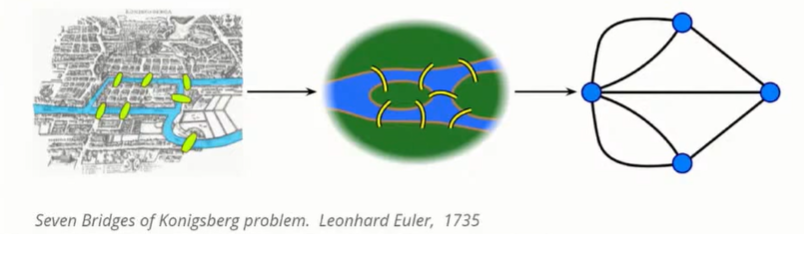
\includegraphics[width=\linewidth,keepaspectratio]{neo4j4}
\end{center}	  

{\tiny (Ref: Introduction to Neo4j - a hands-on crash course - neo4j)}
\end{frame}


%%%%%%%%%%%%%%%%%%%%%%%%%%%%%%%%%%%%%%%%%%%%%%%%%%%%%%%%%%%%%%%%%%%%%%%%%%%%%%%%%%
\begin{frame}\frametitle{Graph Theory}

\begin{itemize}
\item 
\end{itemize}



{\tiny (Ref: A Little Graph Theory for the Busy Developer - Jim Webber GraphConnect London 2013)}
\end{frame}

%%%%%%%%%%%%%%%%%%%%%%%%%%%%%%%%%%%%%%%%%%%%%%%%%%%%%%%%%%%
\begin{frame}[fragile]\frametitle{ Graph-structured Data Are Ubiquitous }

\begin{center}
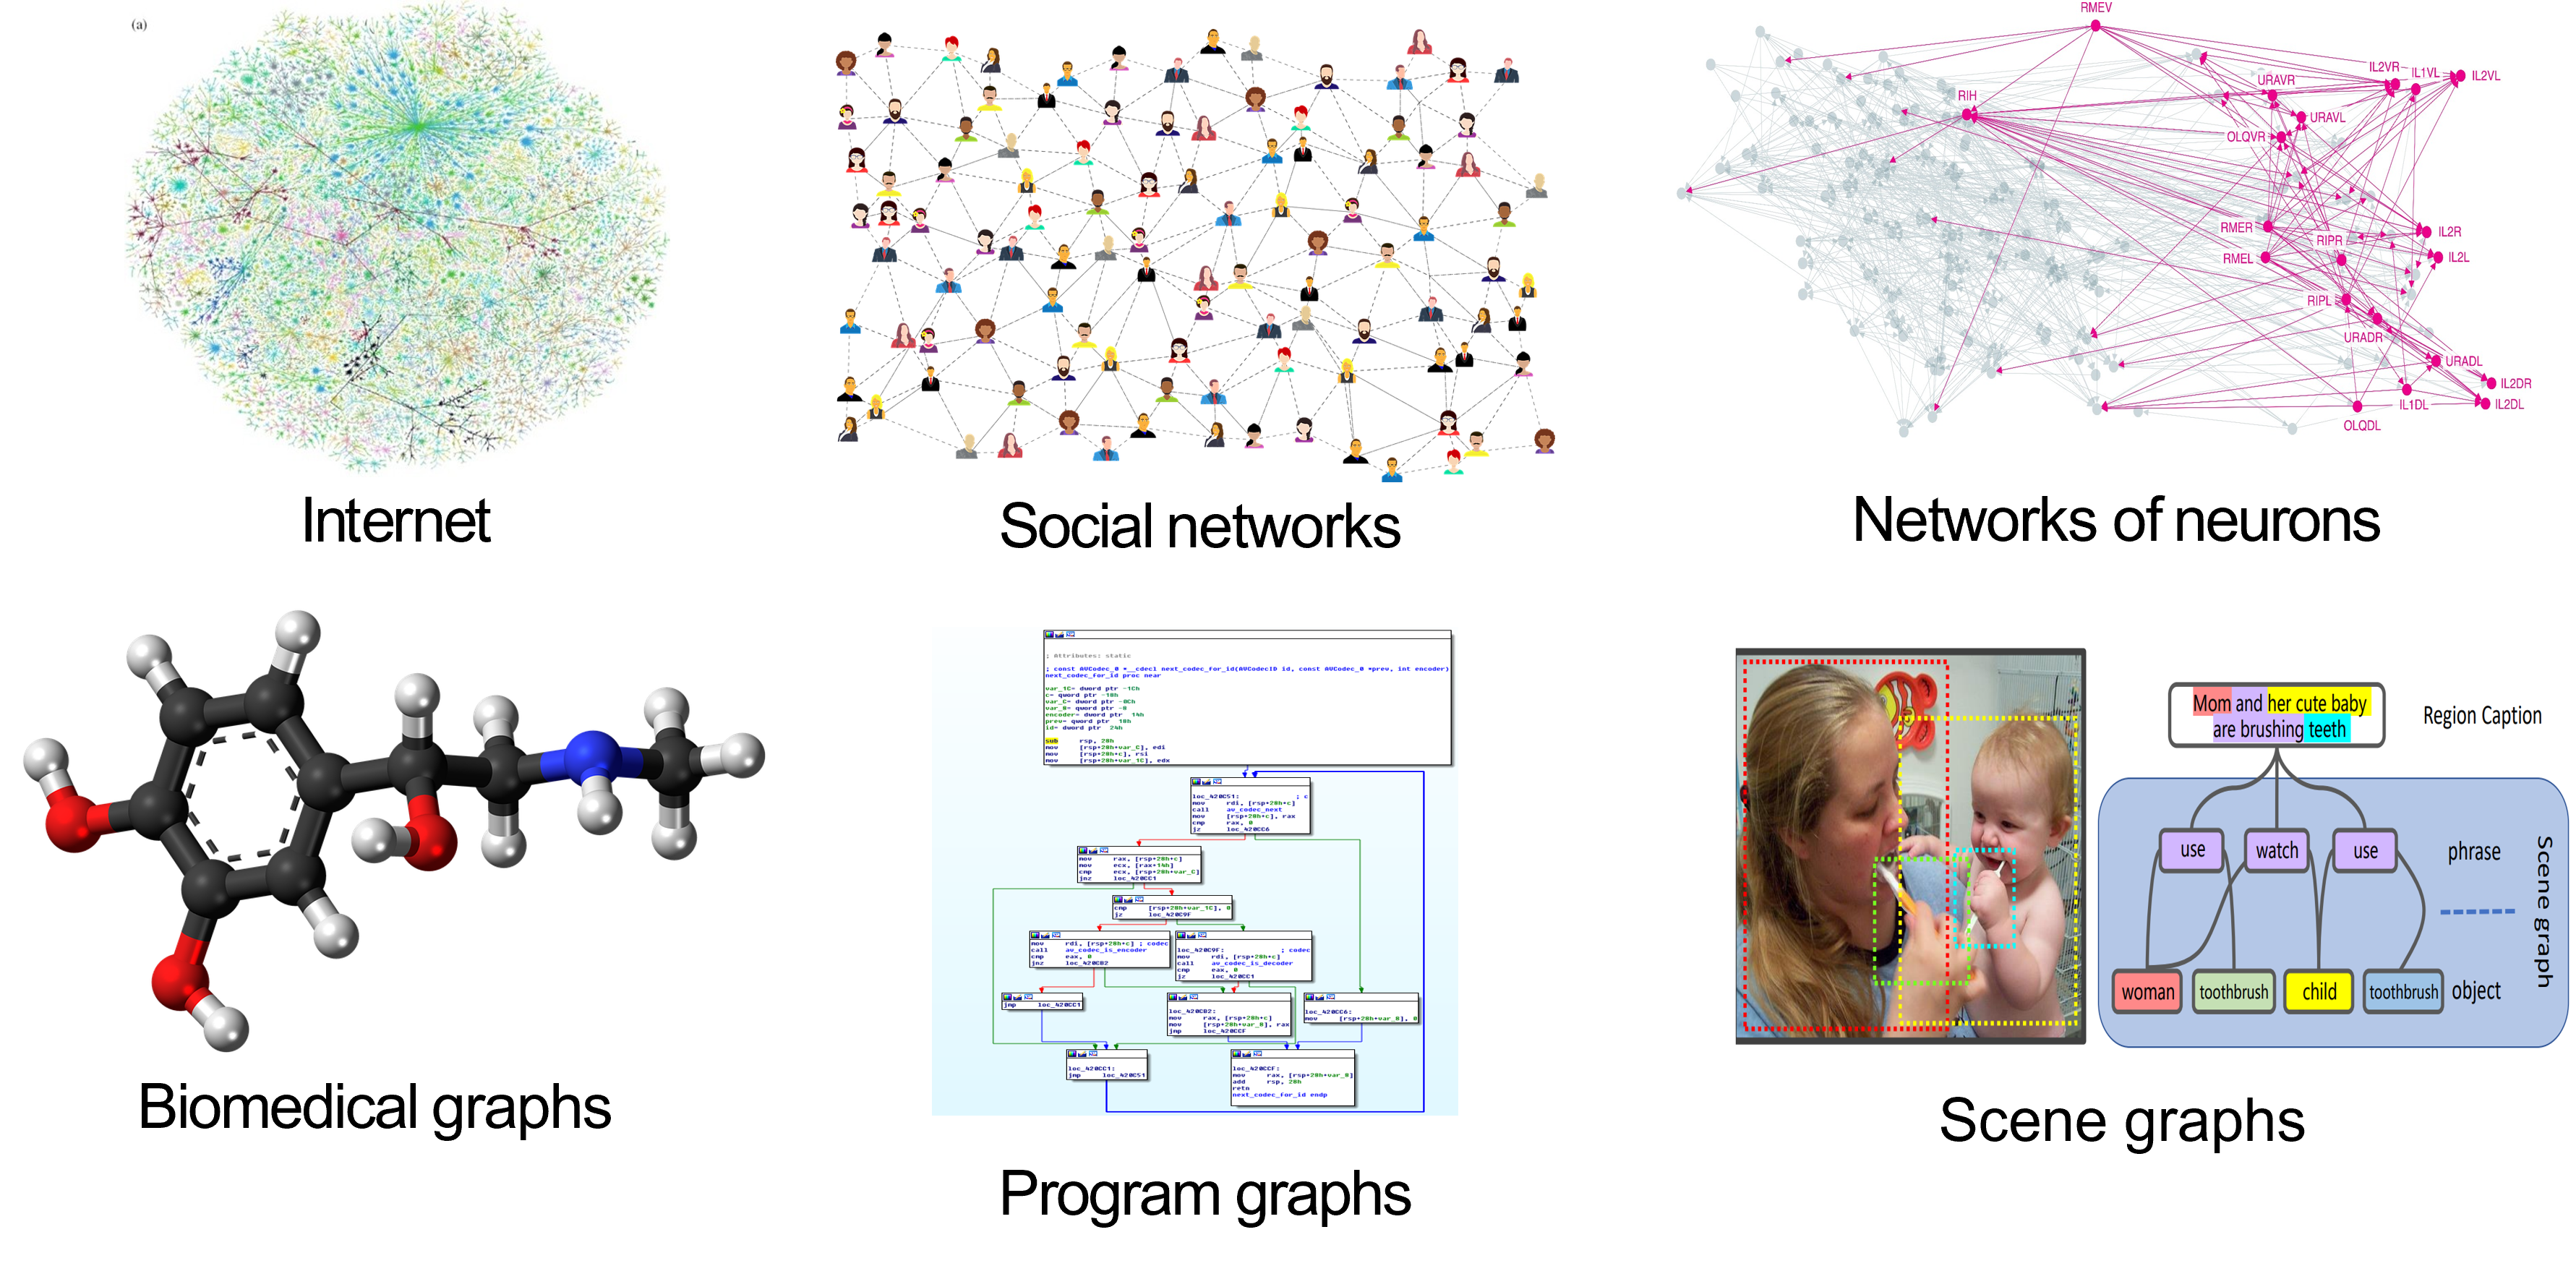
\includegraphics[width=\linewidth,keepaspectratio]{gnn1}
\end{center}	  

\end{frame}

%%%%%%%%%%%%%%%%%%%%%%%%%%%%%%%%%%%%%%%%%%%%%%%%%%%%%%%%%%%
\begin{frame}[fragile]\frametitle{}

\begin{center}
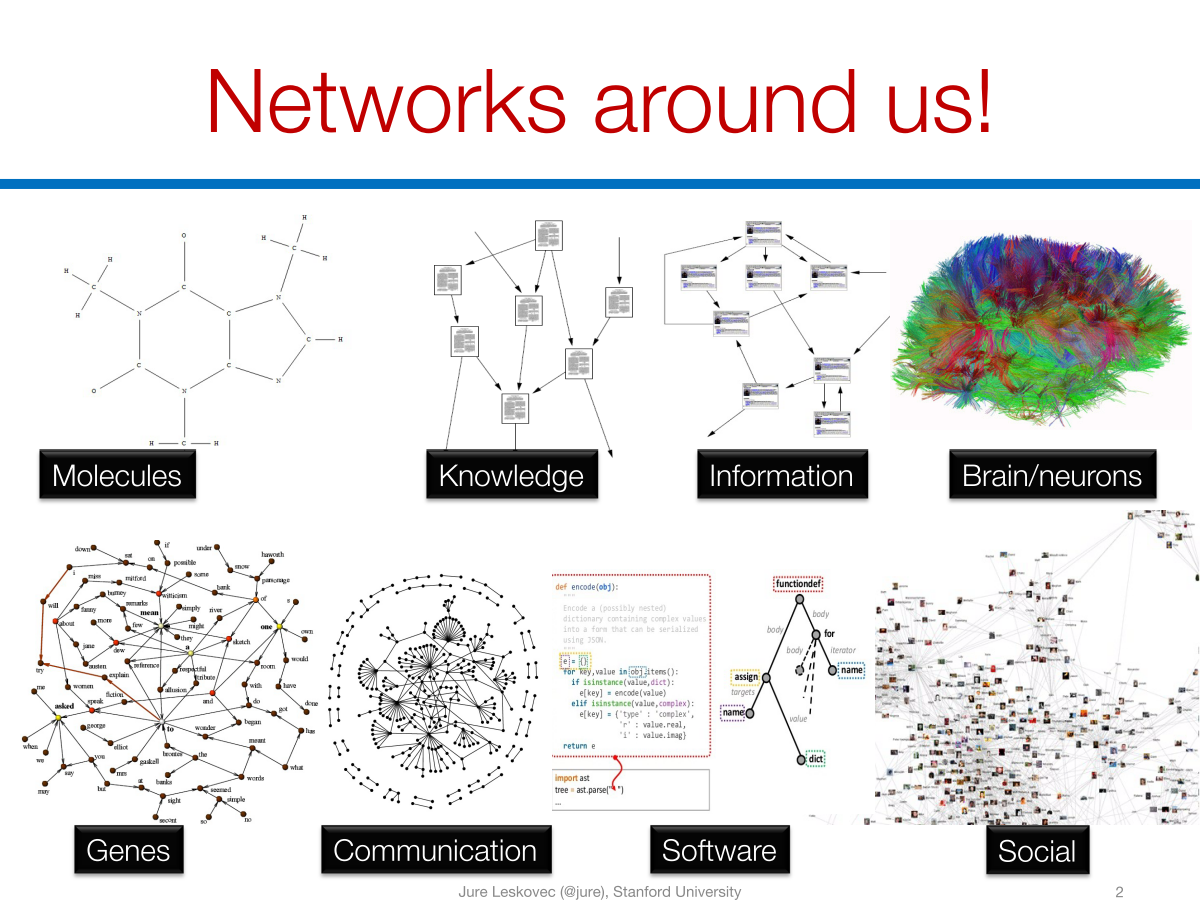
\includegraphics[width=\linewidth,keepaspectratio]{gnn2}
\end{center}	  

\end{frame}

%%%%%%%%%%%%%%%%%%%%%%%%%%%%%%%%%%%%%%%%%%%%%%%%%%%%%%%%%%%
\begin{frame}[fragile]\frametitle{}

\begin{center}
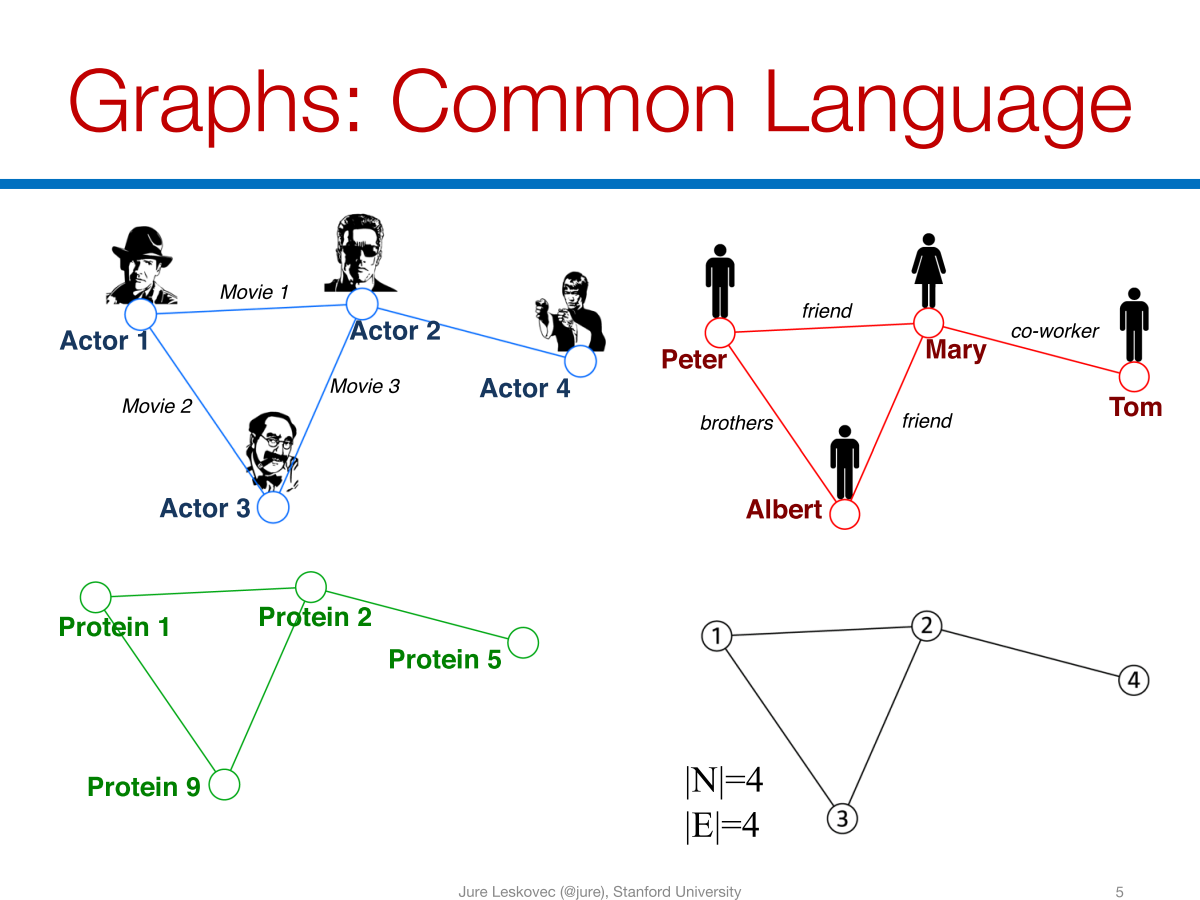
\includegraphics[width=\linewidth,keepaspectratio]{gnn3}
\end{center}	  

\end{frame}

%%%%%%%%%%%%%%%%%%%%%%%%%%%%%%%%%%%%%%%%%%%%%%%%%%%%%%%%%%%
\begin{frame}[fragile]\frametitle{Graphs: A Universal Language }

\begin{center}
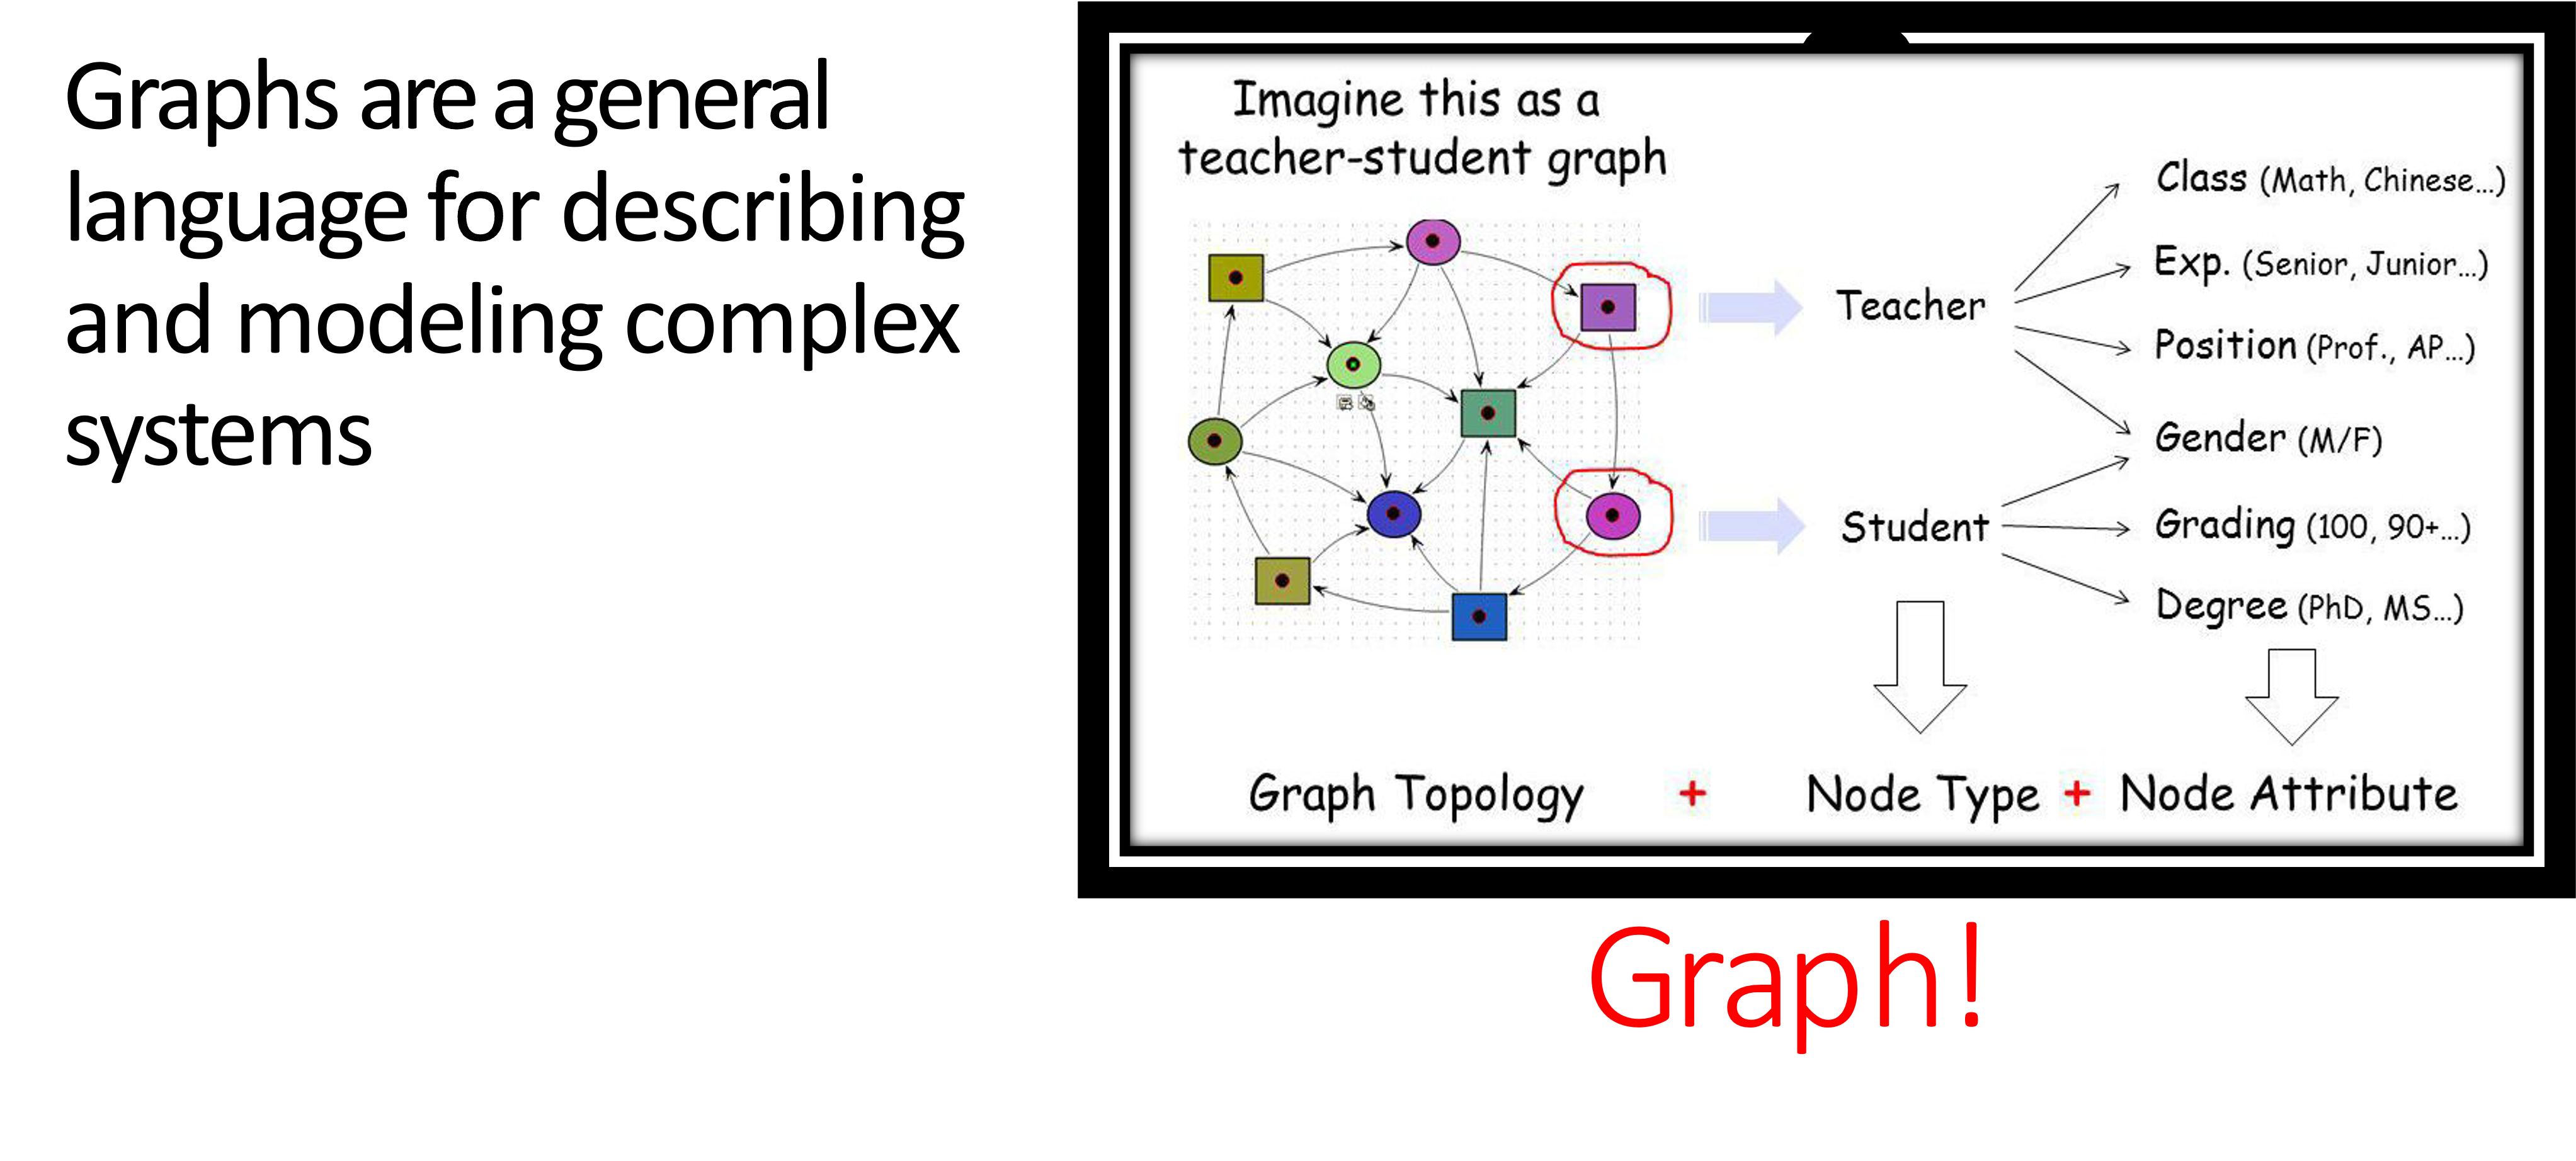
\includegraphics[width=\linewidth,keepaspectratio]{gnn4}
\end{center}	  

\end{frame}


%%%%%%%%%%%%%%%%%%%%%%%%%%%%%%%%%%%%%%%%%%%%%%%%%%%%%%%%%%%
\begin{frame}[fragile]\frametitle{Data as Graphs - Explicit }

\begin{center}
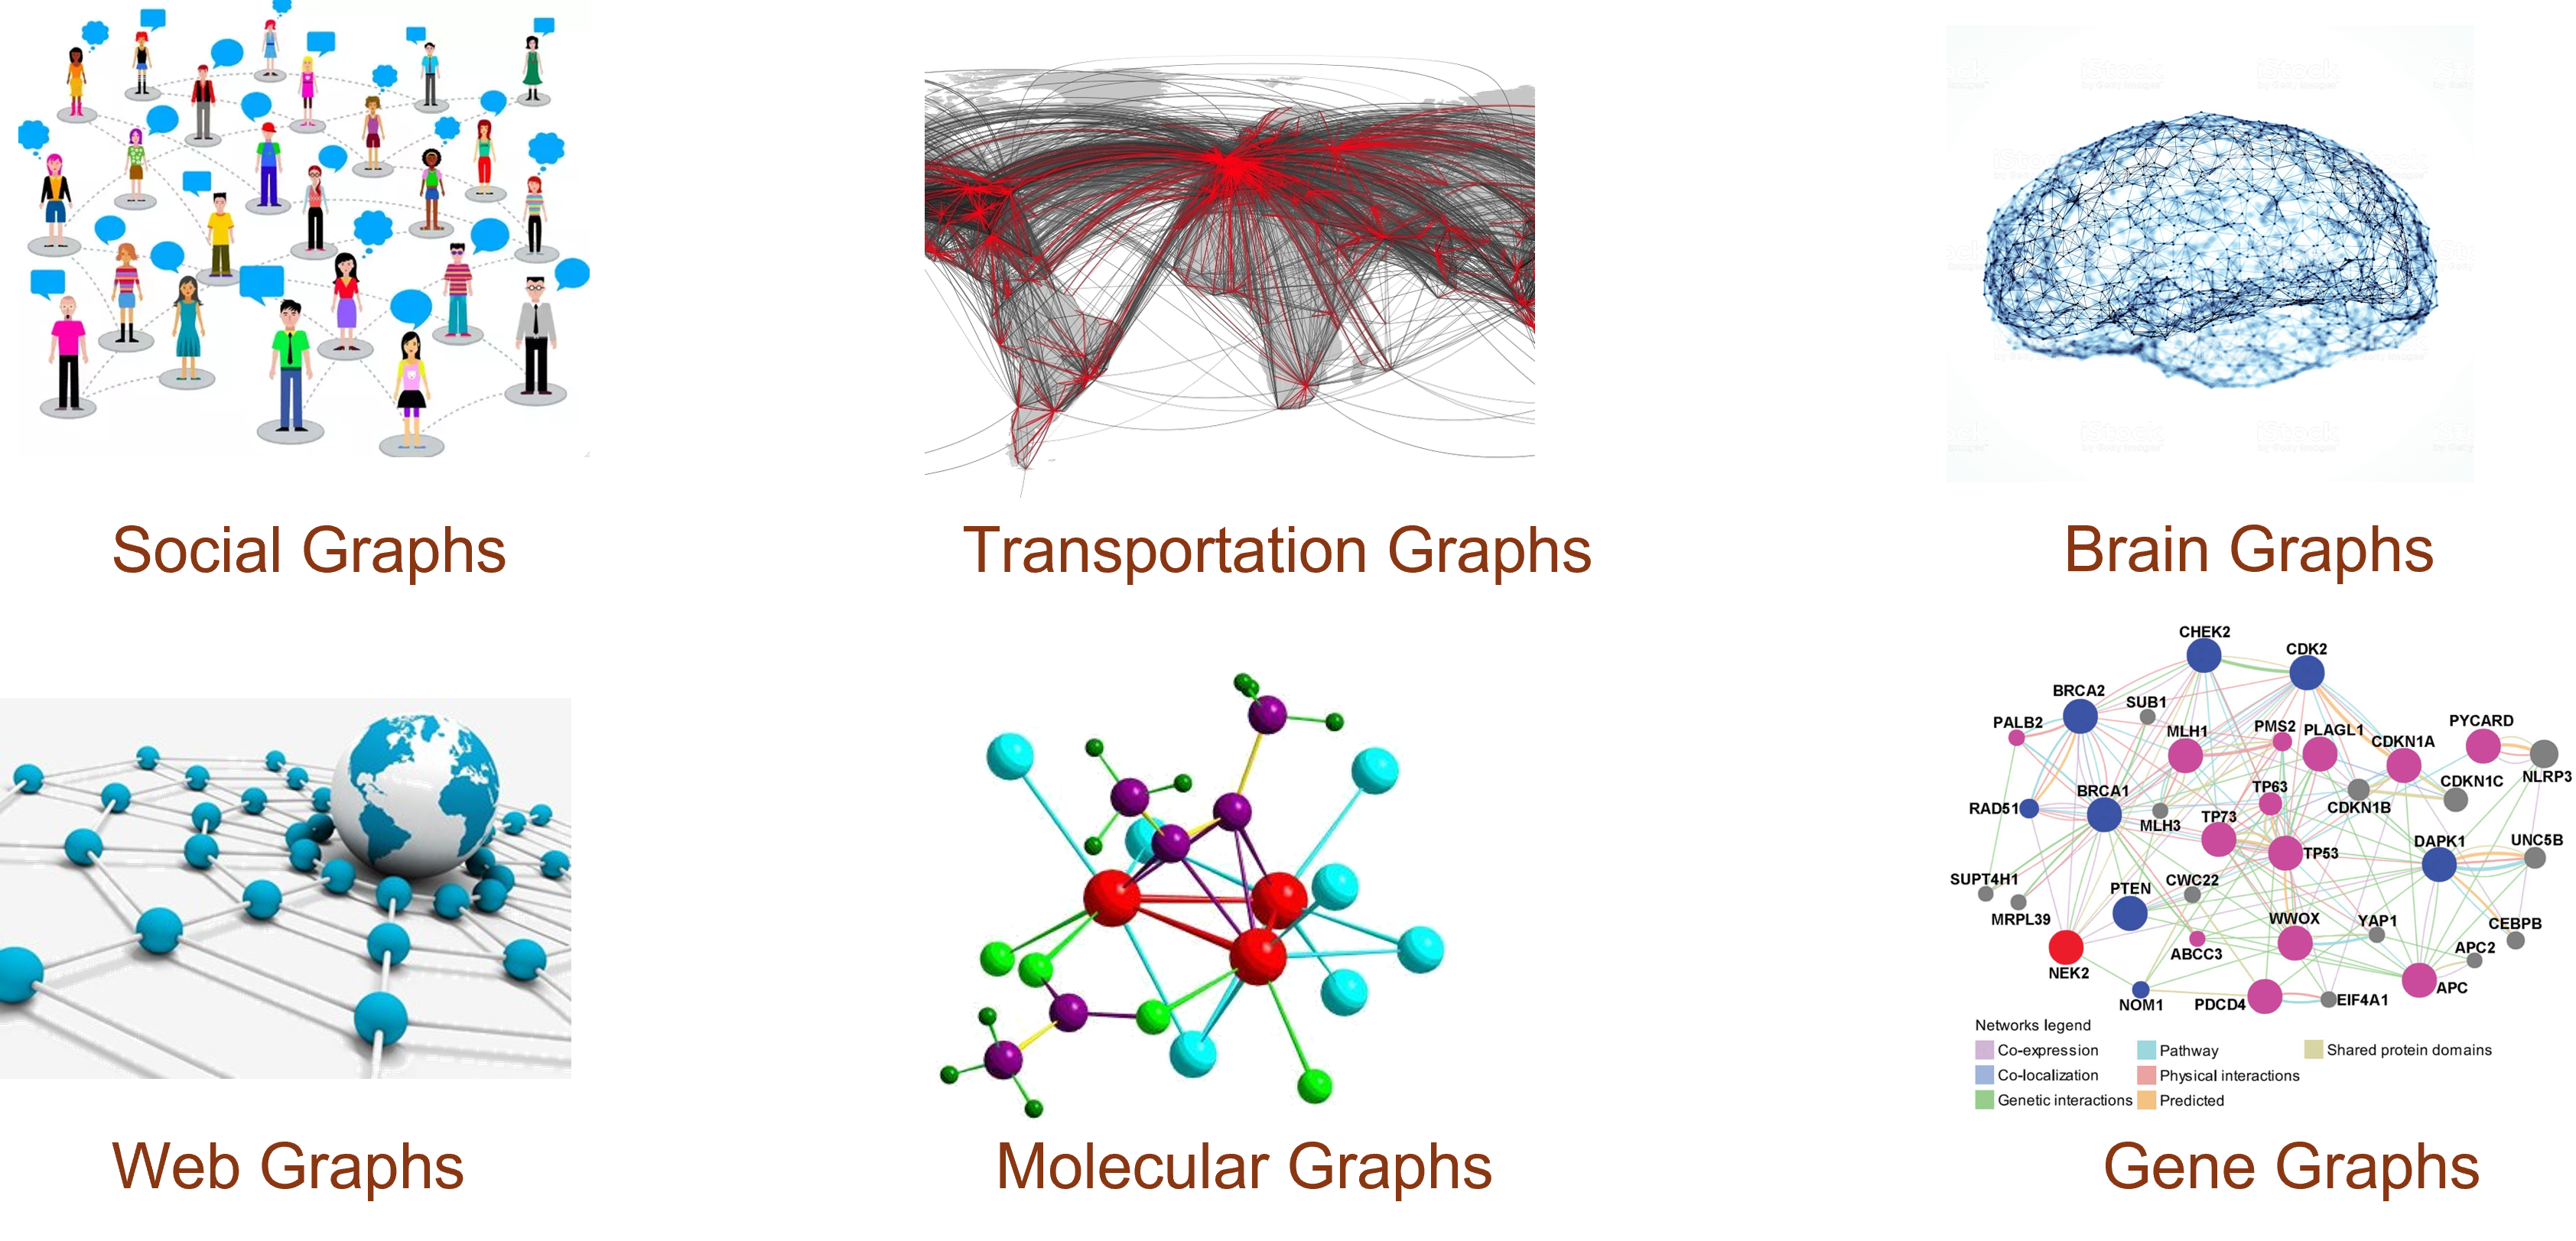
\includegraphics[width=\linewidth,keepaspectratio]{gnn5}
\end{center}	  

\end{frame}

%%%%%%%%%%%%%%%%%%%%%%%%%%%%%%%%%%%%%%%%%%%%%%%%%%%%%%%%%%%
\begin{frame}[fragile]\frametitle{Data as Graphs - Implicit }

\begin{center}
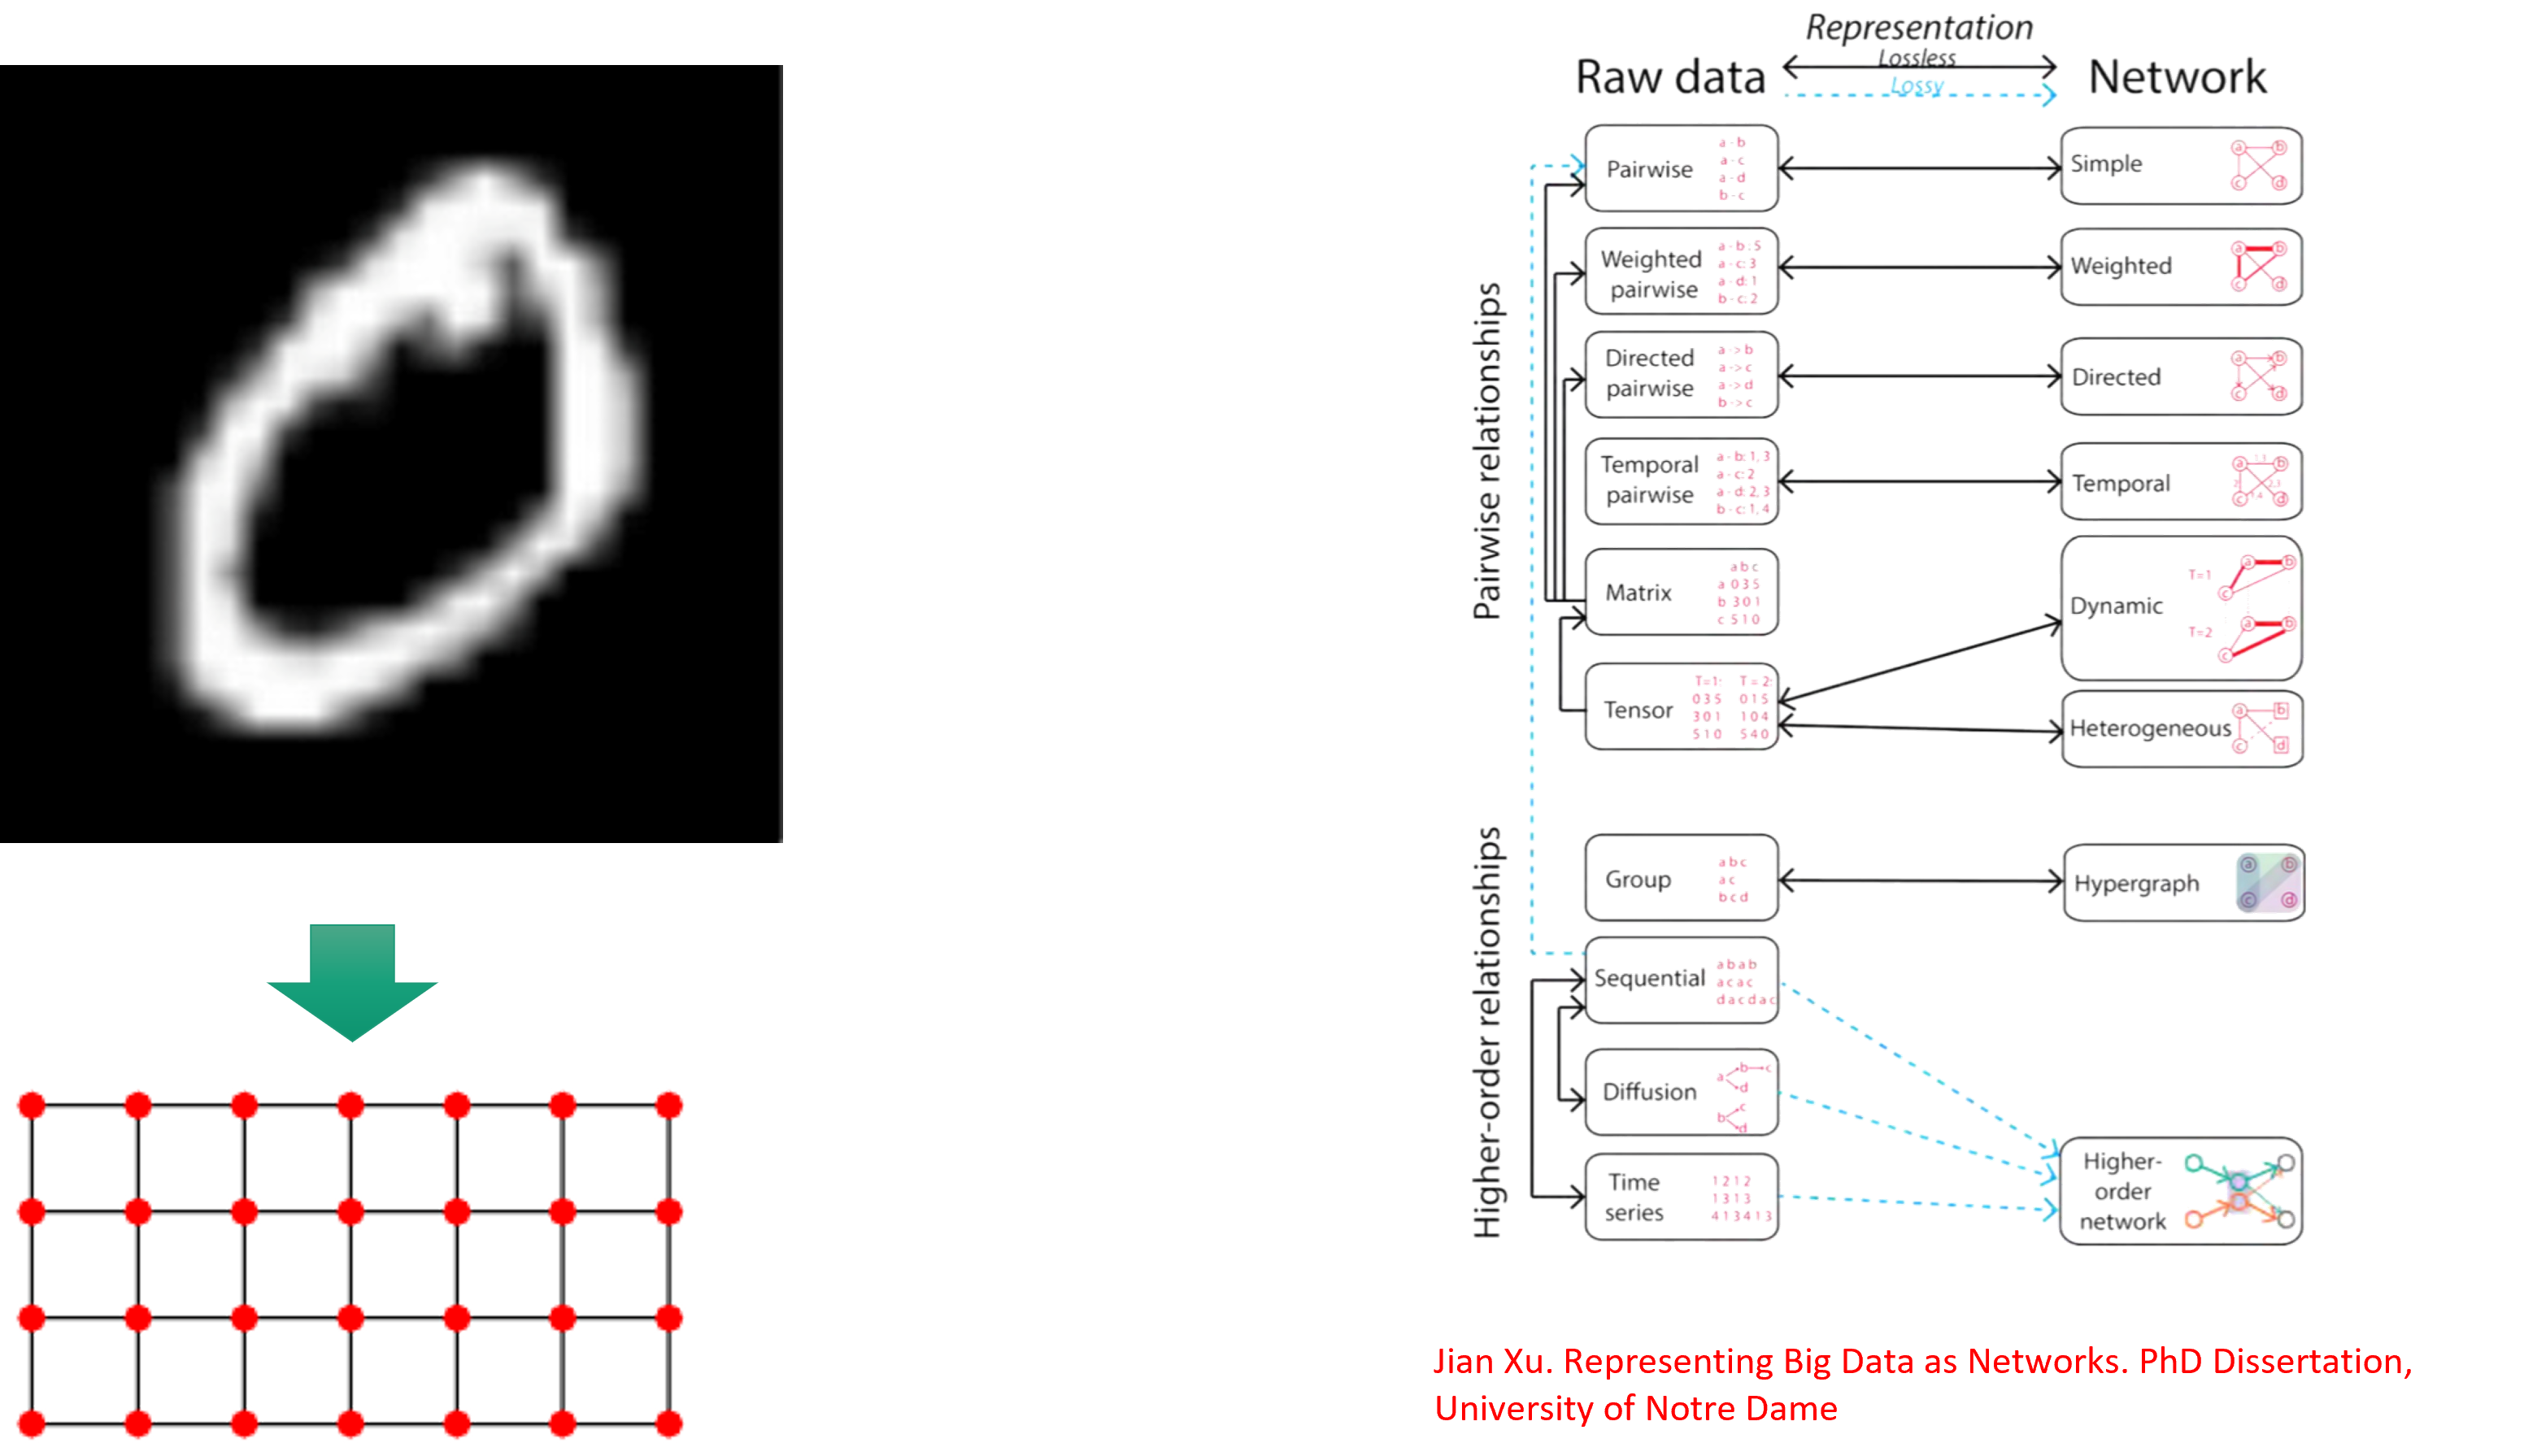
\includegraphics[width=\linewidth,keepaspectratio]{gnn6}
\end{center}	  

\end{frame}



%%%%%%%%%%%%%%%%%%%%%%%%%%%%%%%%%%%%%%%%%%%%%%%%%%%%%%%%%%%
\begin{frame}[fragile]\frametitle{}

\begin{center}
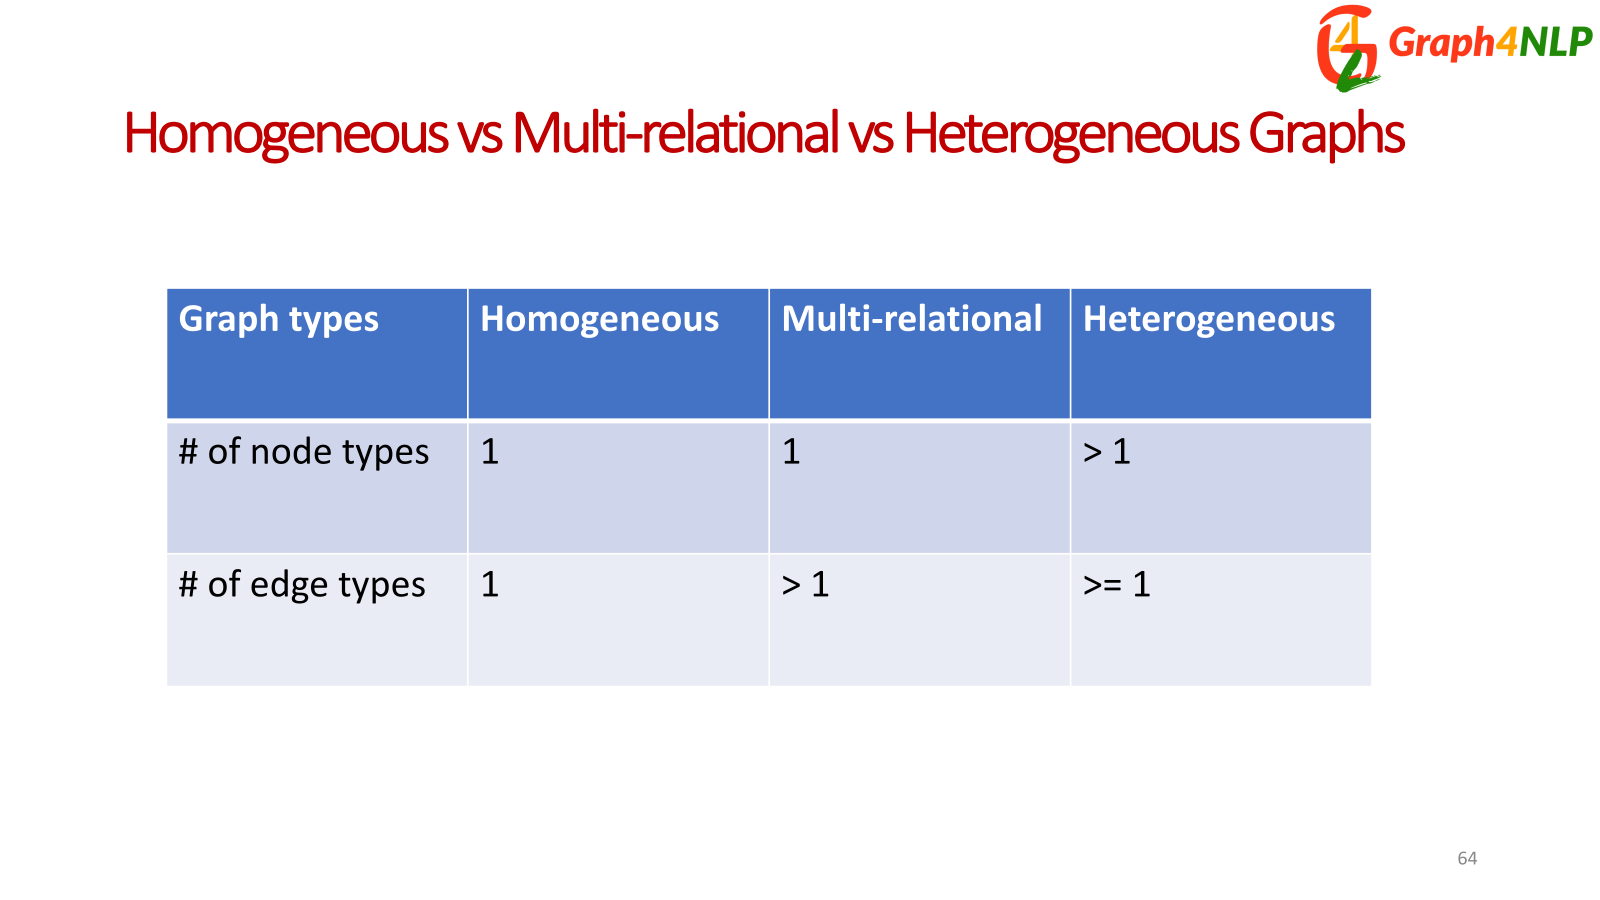
\includegraphics[width=\linewidth,keepaspectratio]{gnn8}
\end{center}	  

\end{frame}


%%%%%%%%%%%%%%%%%%%%%%%%%%%%%%%%%%%%%%%%%%%%%%%%%%%%%%%%%%%%%%%%%%%%%%%%%%%%%%%%%%
\begin{frame}\frametitle{Graph Components}

\begin{itemize}
\item Node (Vertex): A must data element for constructing a graph
\item Relationship (Edge) : Link between two nodes, can have direction and type.
\item Label: Node category/type such as PERSON, ORG, etc. One node can have many types.
\item Properties: Attributes or fields in Nodes or Edges, eg. A node can have Label PERSON and Property such as ``name: Jane''
\end{itemize}



{\tiny (Ref: Introduction to Neo4j - a hands-on crash course - neo4j)}
\end{frame}


%%%%%%%%%%%%%%%%%%%%%%%%%%%%%%%%%%%%%%%%%%%%%%%%%%%%%%%%%%%%%%%%%%%%%%%%%%%%%%%%%%
\begin{frame}\frametitle{Nodes}


\begin{center}
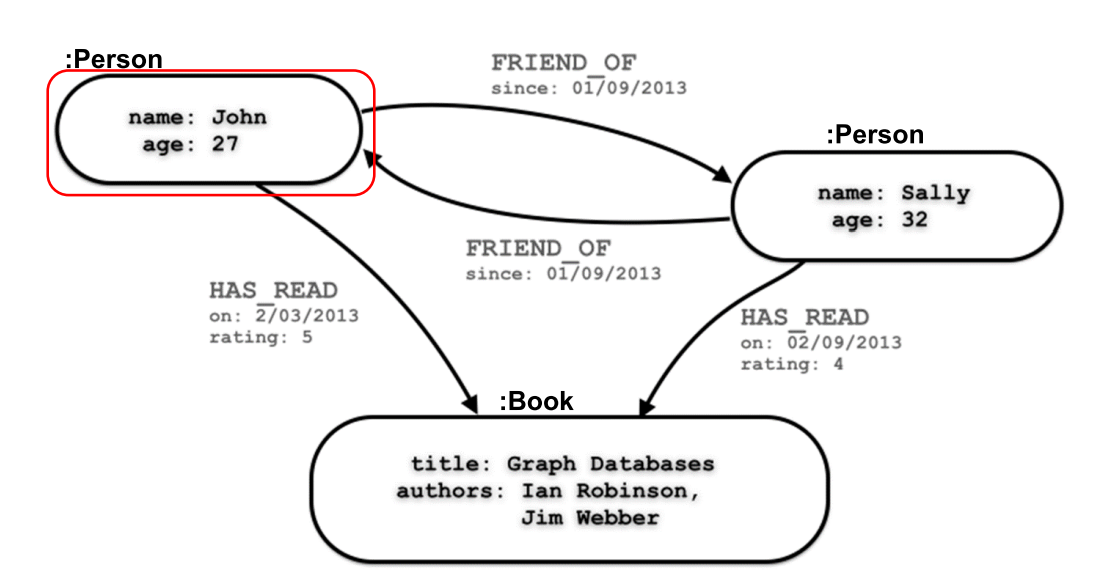
\includegraphics[width=\linewidth,keepaspectratio]{neo4j33}
\end{center}	

{\tiny (Ref: CIS 6930 - Advanced Databases - Neo4j )}
\end{frame}


%%%%%%%%%%%%%%%%%%%%%%%%%%%%%%%%%%%%%%%%%%%%%%%%%%%%%%%%%%%%%%%%%%%%%%%%%%%%%%%%%%
\begin{frame}\frametitle{Relationships}


\begin{center}
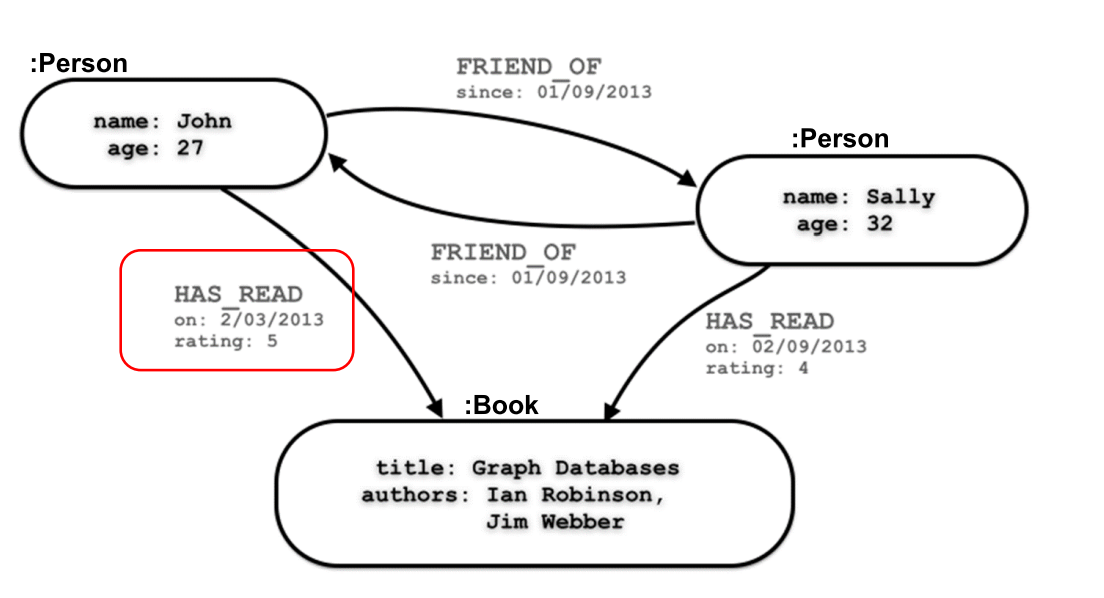
\includegraphics[width=\linewidth,keepaspectratio]{neo4j34}
\end{center}	

{\tiny (Ref: CIS 6930 - Advanced Databases - Neo4j )}
\end{frame}

%%%%%%%%%%%%%%%%%%%%%%%%%%%%%%%%%%%%%%%%%%%%%%%%%%%%%%%%%%%%%%%%%%%%%%%%%%%%%%%%%%
\begin{frame}\frametitle{Properties}


\begin{center}
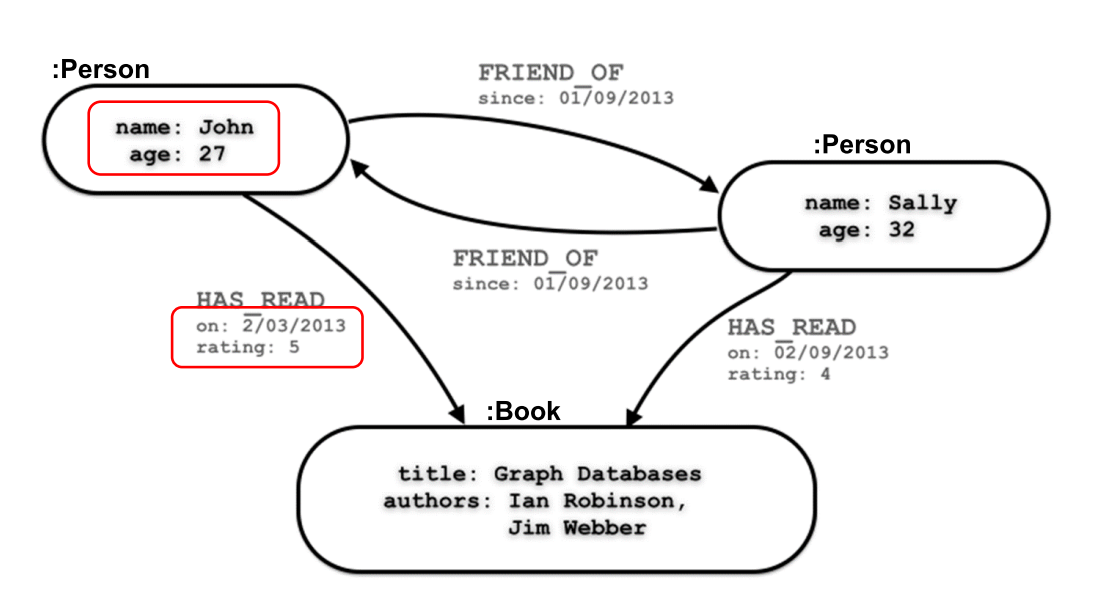
\includegraphics[width=\linewidth,keepaspectratio]{neo4j35}
\end{center}	

{\tiny (Ref: CIS 6930 - Advanced Databases - Neo4j )}
\end{frame}


%%%%%%%%%%%%%%%%%%%%%%%%%%%%%%%%%%%%%%%%%%%%%%%%%%%%%%%%%%%%%%%%%%%%%%%%%%%%%%%%%%
\begin{frame}\frametitle{Labels}


\begin{center}
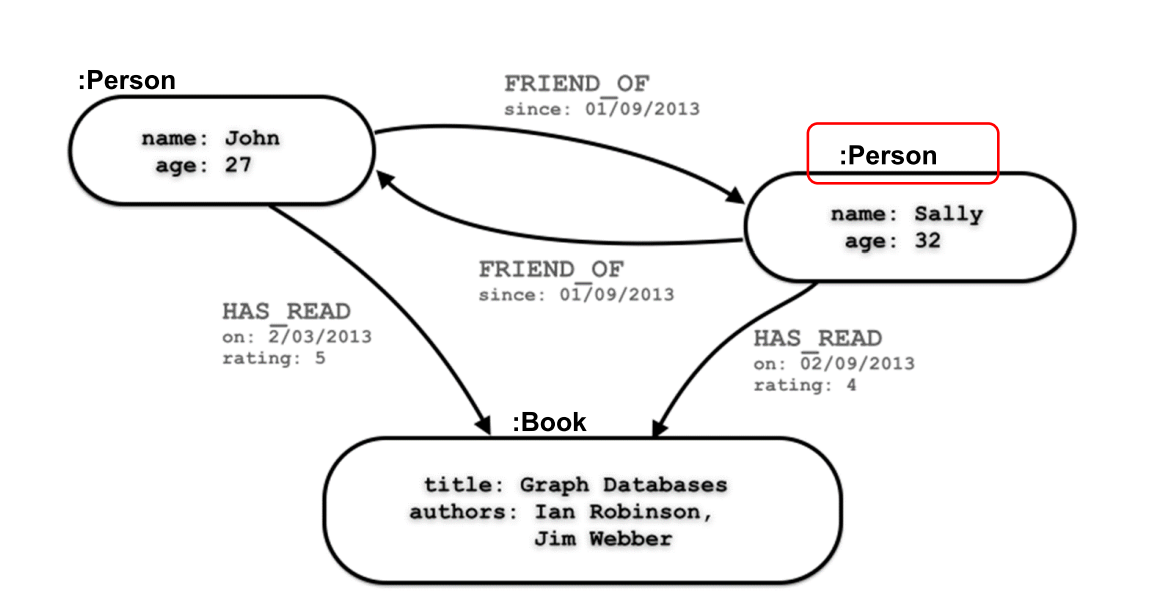
\includegraphics[width=\linewidth,keepaspectratio]{neo4j36}
\end{center}	

{\tiny (Ref: CIS 6930 - Advanced Databases - Neo4j )}
\end{frame}


%%%%%%%%%%%%%%%%%%%%%%%%%%%%%%%%%%%%%%%%%%%%%%%%%%%%%%%%%%%
\begin{frame}[fragile]\frametitle{Graphs and features}

\begin{center}
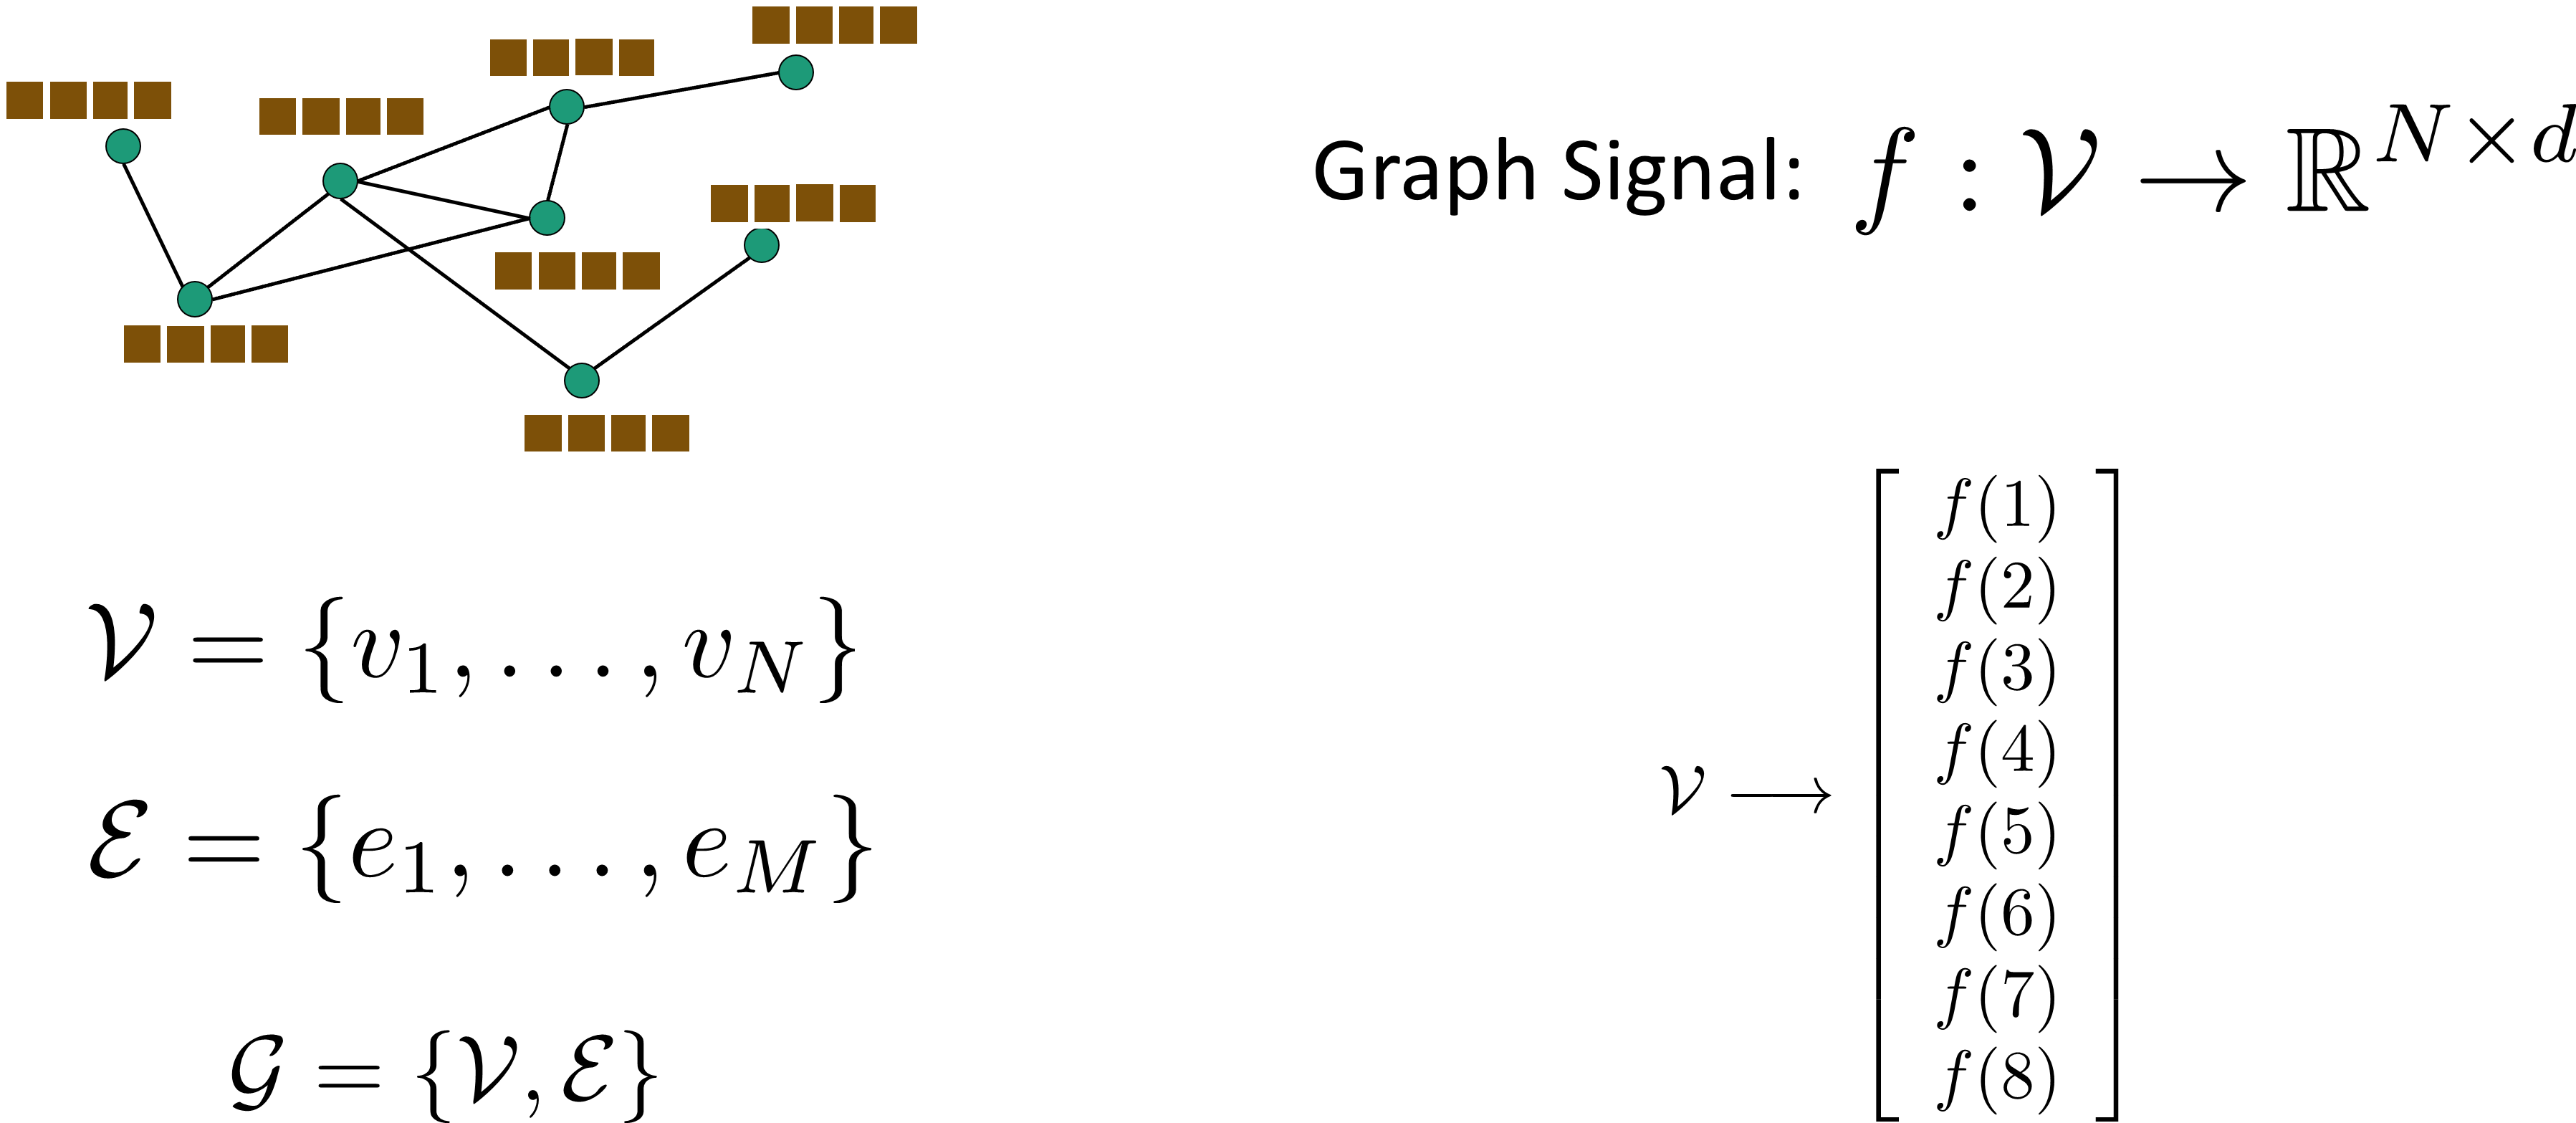
\includegraphics[width=\linewidth,keepaspectratio]{gnn9}
\end{center}	  

\end{frame}

%%%%%%%%%%%%%%%%%%%%%%%%%%%%%%%%%%%%%%%%%%%%%%%%%%%%%%%%%%%
\begin{frame}[fragile]\frametitle{Matrix Representations of Graphs}

\begin{center}
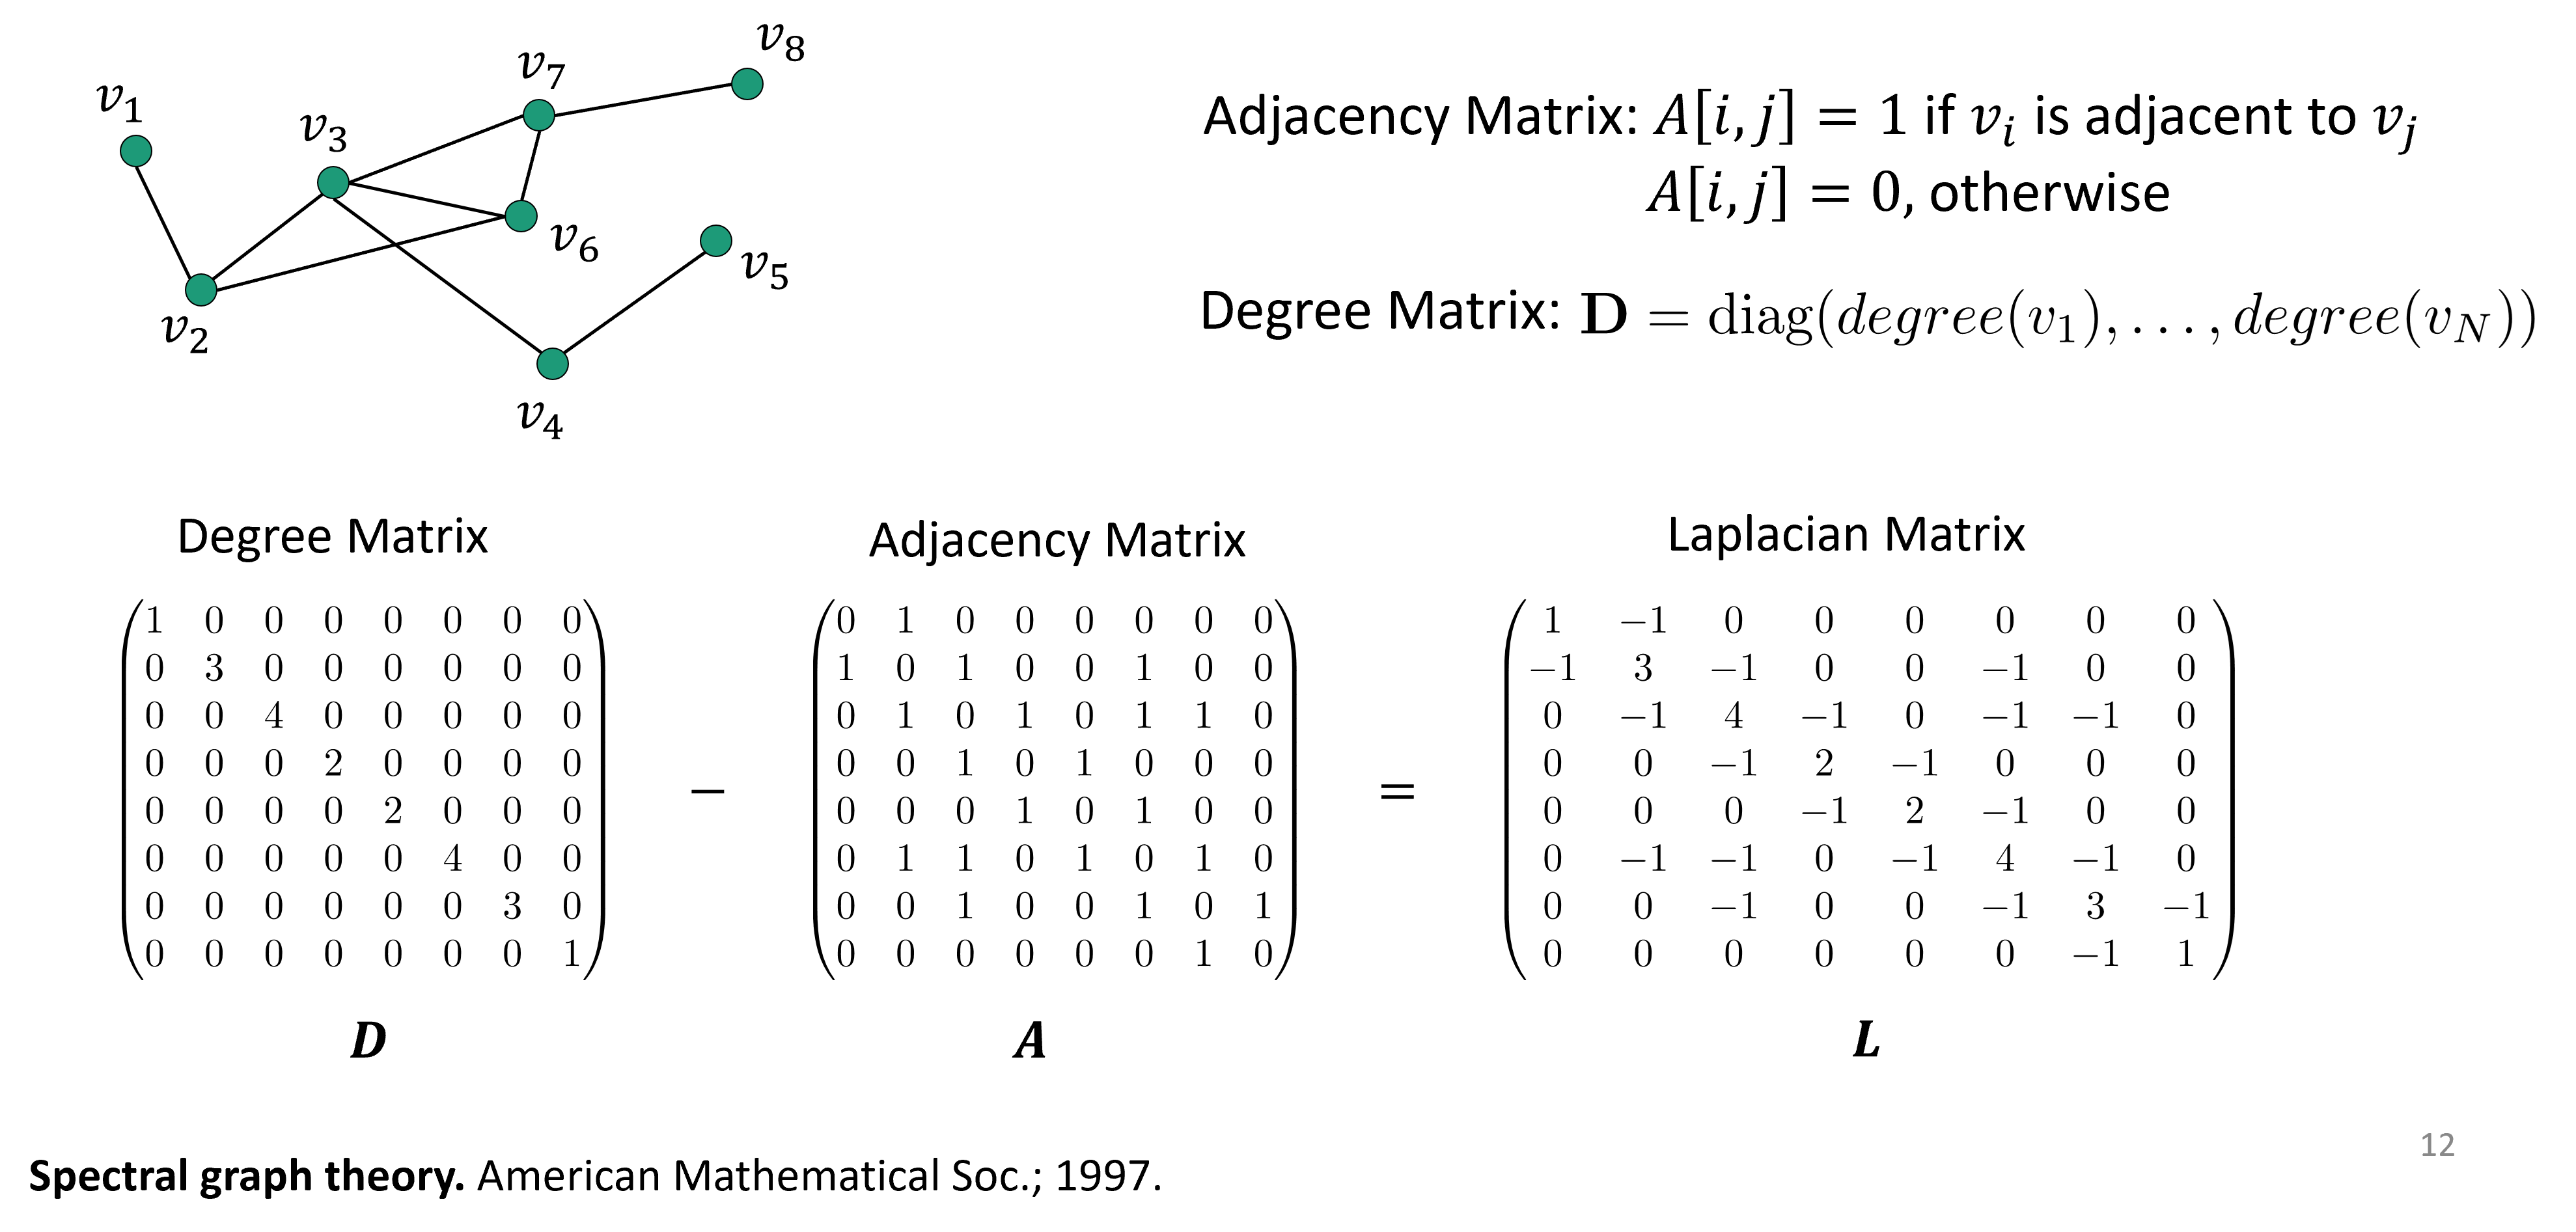
\includegraphics[width=\linewidth,keepaspectratio]{gnn10}
\end{center}	  

\end{frame}

%%%%%%%%%%%%%%%%%%%%%%%%%%%%%%%%%%%%%%%%%%%%%%%%%%%%%%%%%%%
\begin{frame}[fragile]\frametitle{Why Graphs? Why Now?}

\begin{itemize}
\item Universal language for describing complex data: Networks/graphs from science, nature, and technology are more similar than one would expect
\item Shared vocabulary between fields: Computer Science, Social science, Physics, Biology, Economics 
\item Data availability (+ computational challenges): Social/Internet, text, logic, program, bio, health, and medical
\item Impact: Social networking, Social media, Drug design, Event detection, Natural language processing, Computer vision, and Logic reasoning
\end{itemize}

\end{frame}

%%%%%%%%%%%%%%%%%%%%%%%%%%%%%%%%%%%%%%%%%%%%%%%%%%%%%%%%%%%%%%%%%%%%%%%%%%%%%%%%%%
\begin{frame}\frametitle{Identifying good Graph scenarios - 1/4}

Does the problem involve understanding relationships between entities?

Behavioral analysis:

\begin{center}
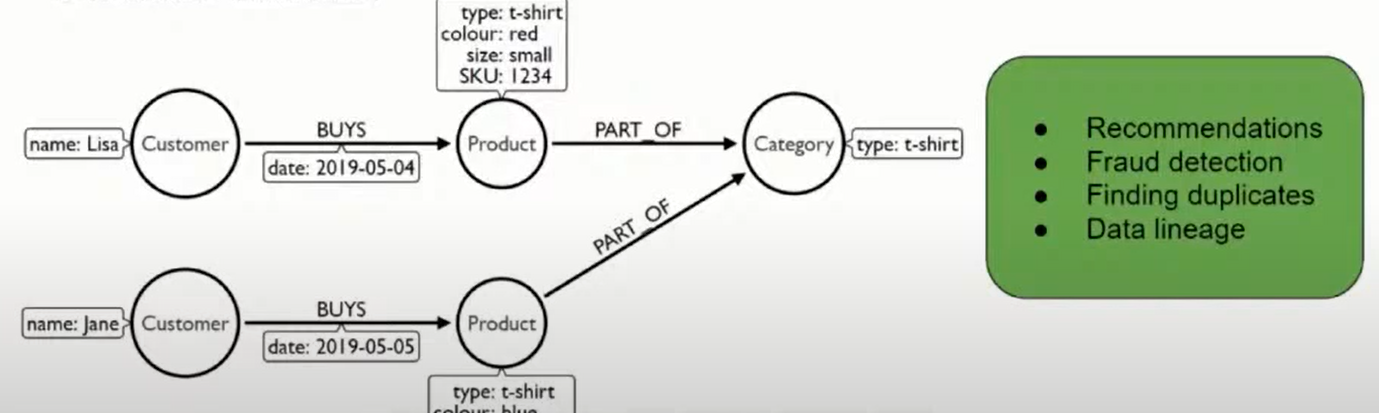
\includegraphics[width=\linewidth,keepaspectratio]{neo4j5}
\end{center}	  

{\tiny (Ref: Introduction to Neo4j - a hands-on crash course - neo4j)}
\end{frame}

%%%%%%%%%%%%%%%%%%%%%%%%%%%%%%%%%%%%%%%%%%%%%%%%%%%%%%%%%%%%%%%%%%%%%%%%%%%%%%%%%%
\begin{frame}\frametitle{Identifying good Graph scenarios - 2/4}

Does the problem involve a lot of self-referencing to the same type of entity?

Org chart of employees:

\begin{center}
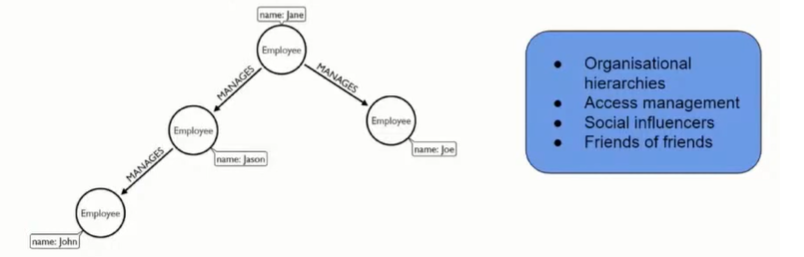
\includegraphics[width=\linewidth,keepaspectratio]{neo4j6}
\end{center}	  

{\tiny (Ref: Introduction to Neo4j - a hands-on crash course - neo4j)}
\end{frame}

%%%%%%%%%%%%%%%%%%%%%%%%%%%%%%%%%%%%%%%%%%%%%%%%%%%%%%%%%%%%%%%%%%%%%%%%%%%%%%%%%%
\begin{frame}\frametitle{Identifying good Graph scenarios - 3/4}

Does the problem explore relationships of varying and unknown depth?

Changes in manufacturing process:

\begin{center}
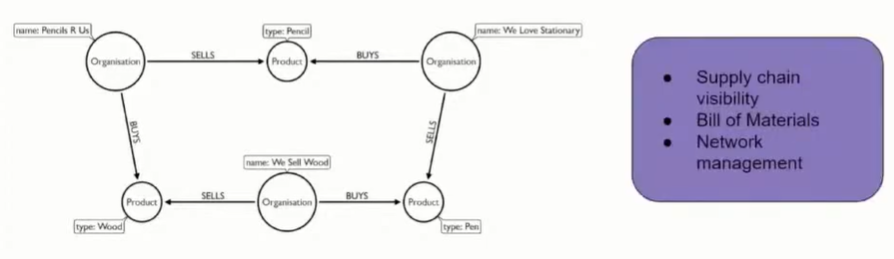
\includegraphics[width=\linewidth,keepaspectratio]{neo4j7}
\end{center}	  

{\tiny (Ref: Introduction to Neo4j - a hands-on crash course - neo4j)}
\end{frame}

%%%%%%%%%%%%%%%%%%%%%%%%%%%%%%%%%%%%%%%%%%%%%%%%%%%%%%%%%%%%%%%%%%%%%%%%%%%%%%%%%%
\begin{frame}\frametitle{Identifying good Graph scenarios - 4/4}

Does the problem involve discovering lots of different routes or paths?

Optimum logistics:

\begin{center}
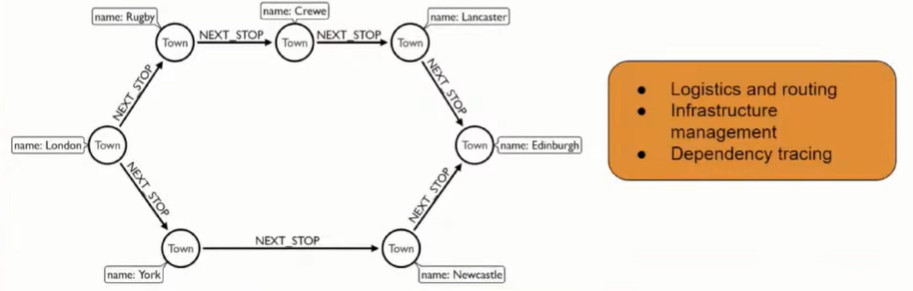
\includegraphics[width=\linewidth,keepaspectratio]{neo4j8}
\end{center}	  

{\tiny (Ref: Introduction to Neo4j - a hands-on crash course - neo4j)}
\end{frame}



\section[MLDL]{Machine/Deep Learning}
%%%%%%%%%%%%%%%%%%%%%%%%%%%%%%%%%%%%%%%%%%%%%%%%%%%%%%%%%%%%%%%%%%%%%%%%%%%%%%%%%%
\begin{frame}[fragile]\frametitle{}
\begin{center}
{\Large Graphs for Machine Learning}
\end{center}
\end{frame}


%%%%%%%%%%%%%%%%%%%%%%%%%%%%%%%%%%%%%%%%%%%%%%%%%%%%%%%%%%%
\begin{frame}[fragile]\frametitle{}

\begin{center}
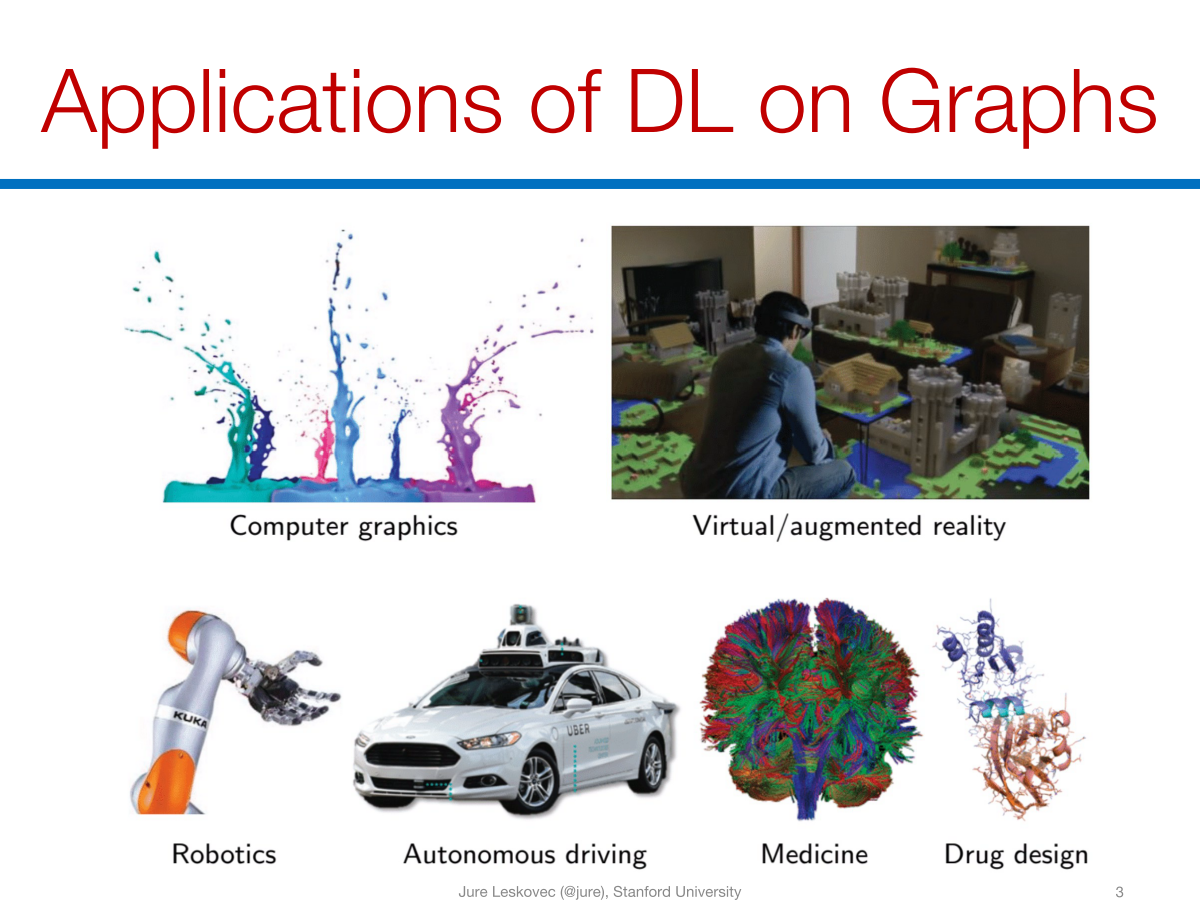
\includegraphics[width=\linewidth,keepaspectratio]{gnn7}
\end{center}	  

\end{frame}


%%%%%%%%%%%%%%%%%%%%%%%%%%%%%%%%%%%%%%%%%%%%%%%%%%%%%%%%%%%
\begin{frame}[fragile]\frametitle{}

\begin{center}
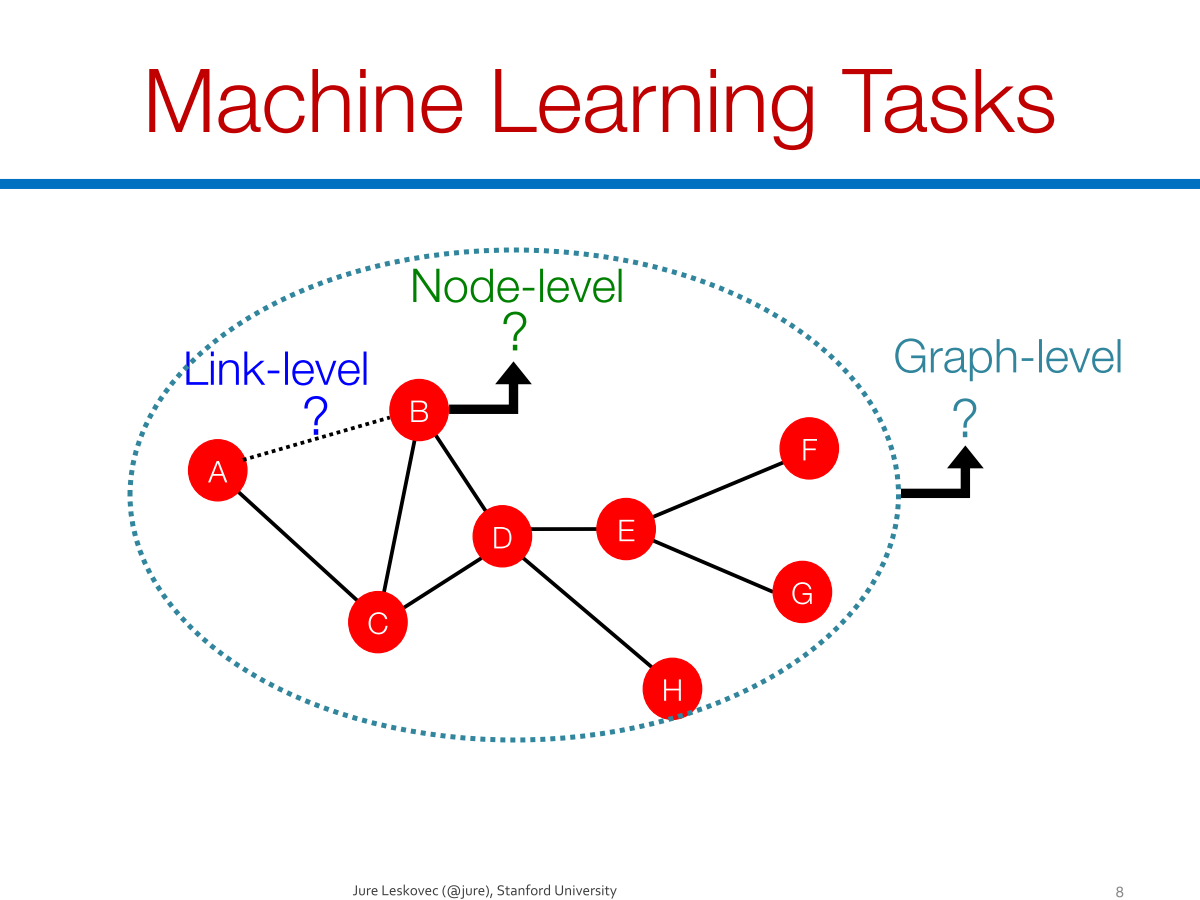
\includegraphics[width=\linewidth,keepaspectratio]{gnn11}
\end{center}	  

\end{frame}

%%%%%%%%%%%%%%%%%%%%%%%%%%%%%%%%%%%%%%%%%%%%%%%%%%%%%%%%%%%
\begin{frame}[fragile]\frametitle{}

\begin{center}
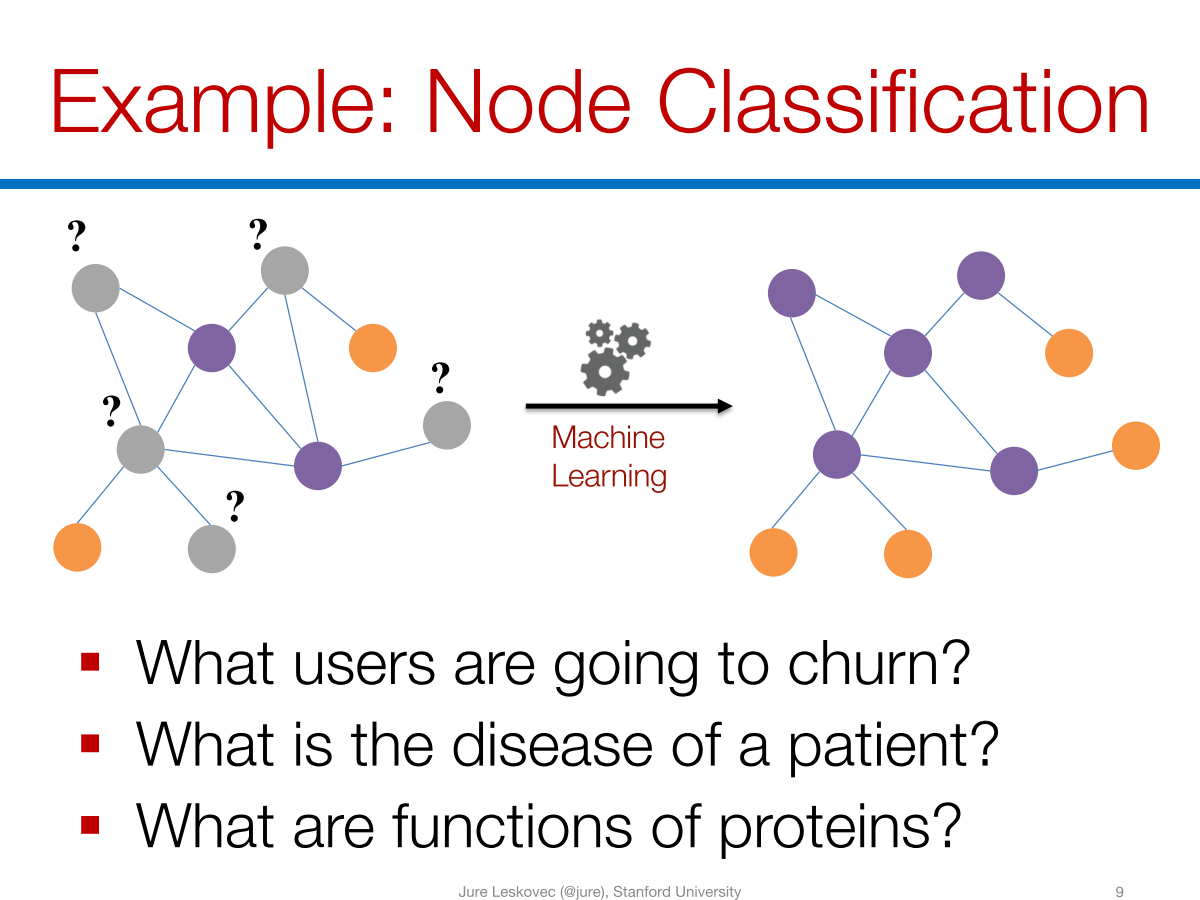
\includegraphics[width=\linewidth,keepaspectratio]{gnn12}
\end{center}	  

\end{frame}


%%%%%%%%%%%%%%%%%%%%%%%%%%%%%%%%%%%%%%%%%%%%%%%%%%%%%%%%%%%
\begin{frame}[fragile]\frametitle{}

\begin{center}
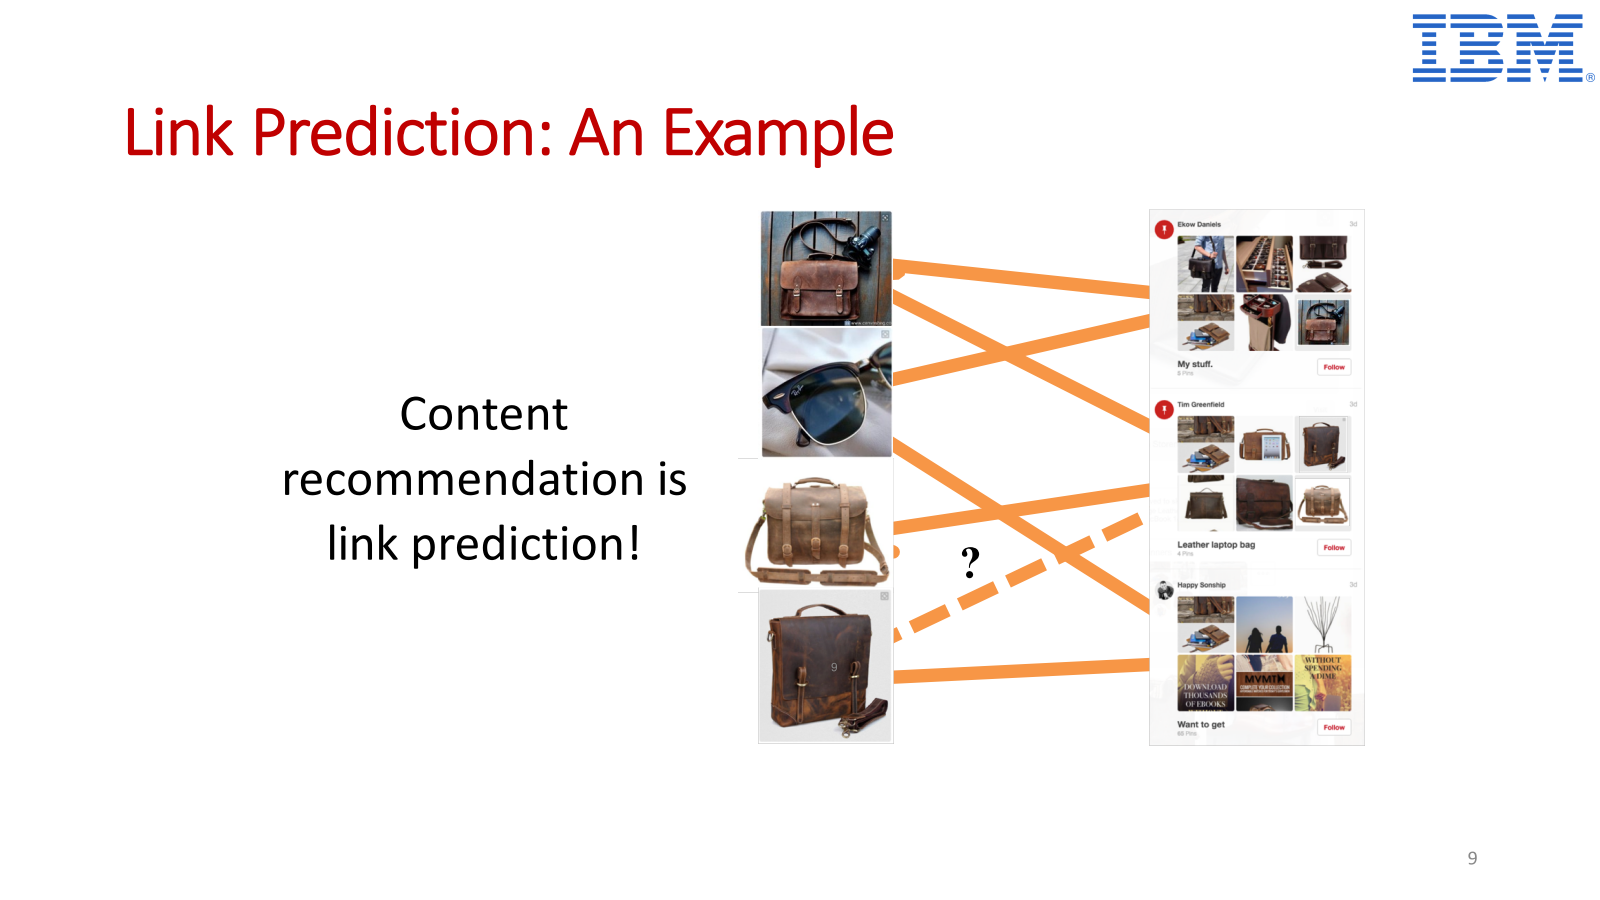
\includegraphics[width=\linewidth,keepaspectratio]{gnn13}
\end{center}	  

\end{frame}


%%%%%%%%%%%%%%%%%%%%%%%%%%%%%%%%%%%%%%%%%%%%%%%%%%%%%%%%%%%
\begin{frame}[fragile]\frametitle{Tasks in graph learning}

\begin{itemize}
\item Node classification
	\begin{itemize}
	\item Detect malicious accounts
	\item Target right customers
	\end{itemize}

\item Link prediction
	\begin{itemize}
	\item Recommendations
	\item Predict missing relations in a knowledge graph
	\end{itemize}

\item Graph classification
	\begin{itemize}
	\item Predict the property of a chemical compound
	\end{itemize}
\end{itemize}

\end{frame}

%%%%%%%%%%%%%%%%%%%%%%%%%%%%%%%%%%%%%%%%%%%%%%%%%%%%%%%%%%%
\begin{frame}[fragile]\frametitle{Tasks on Graph-Structured Data}

\begin{center}
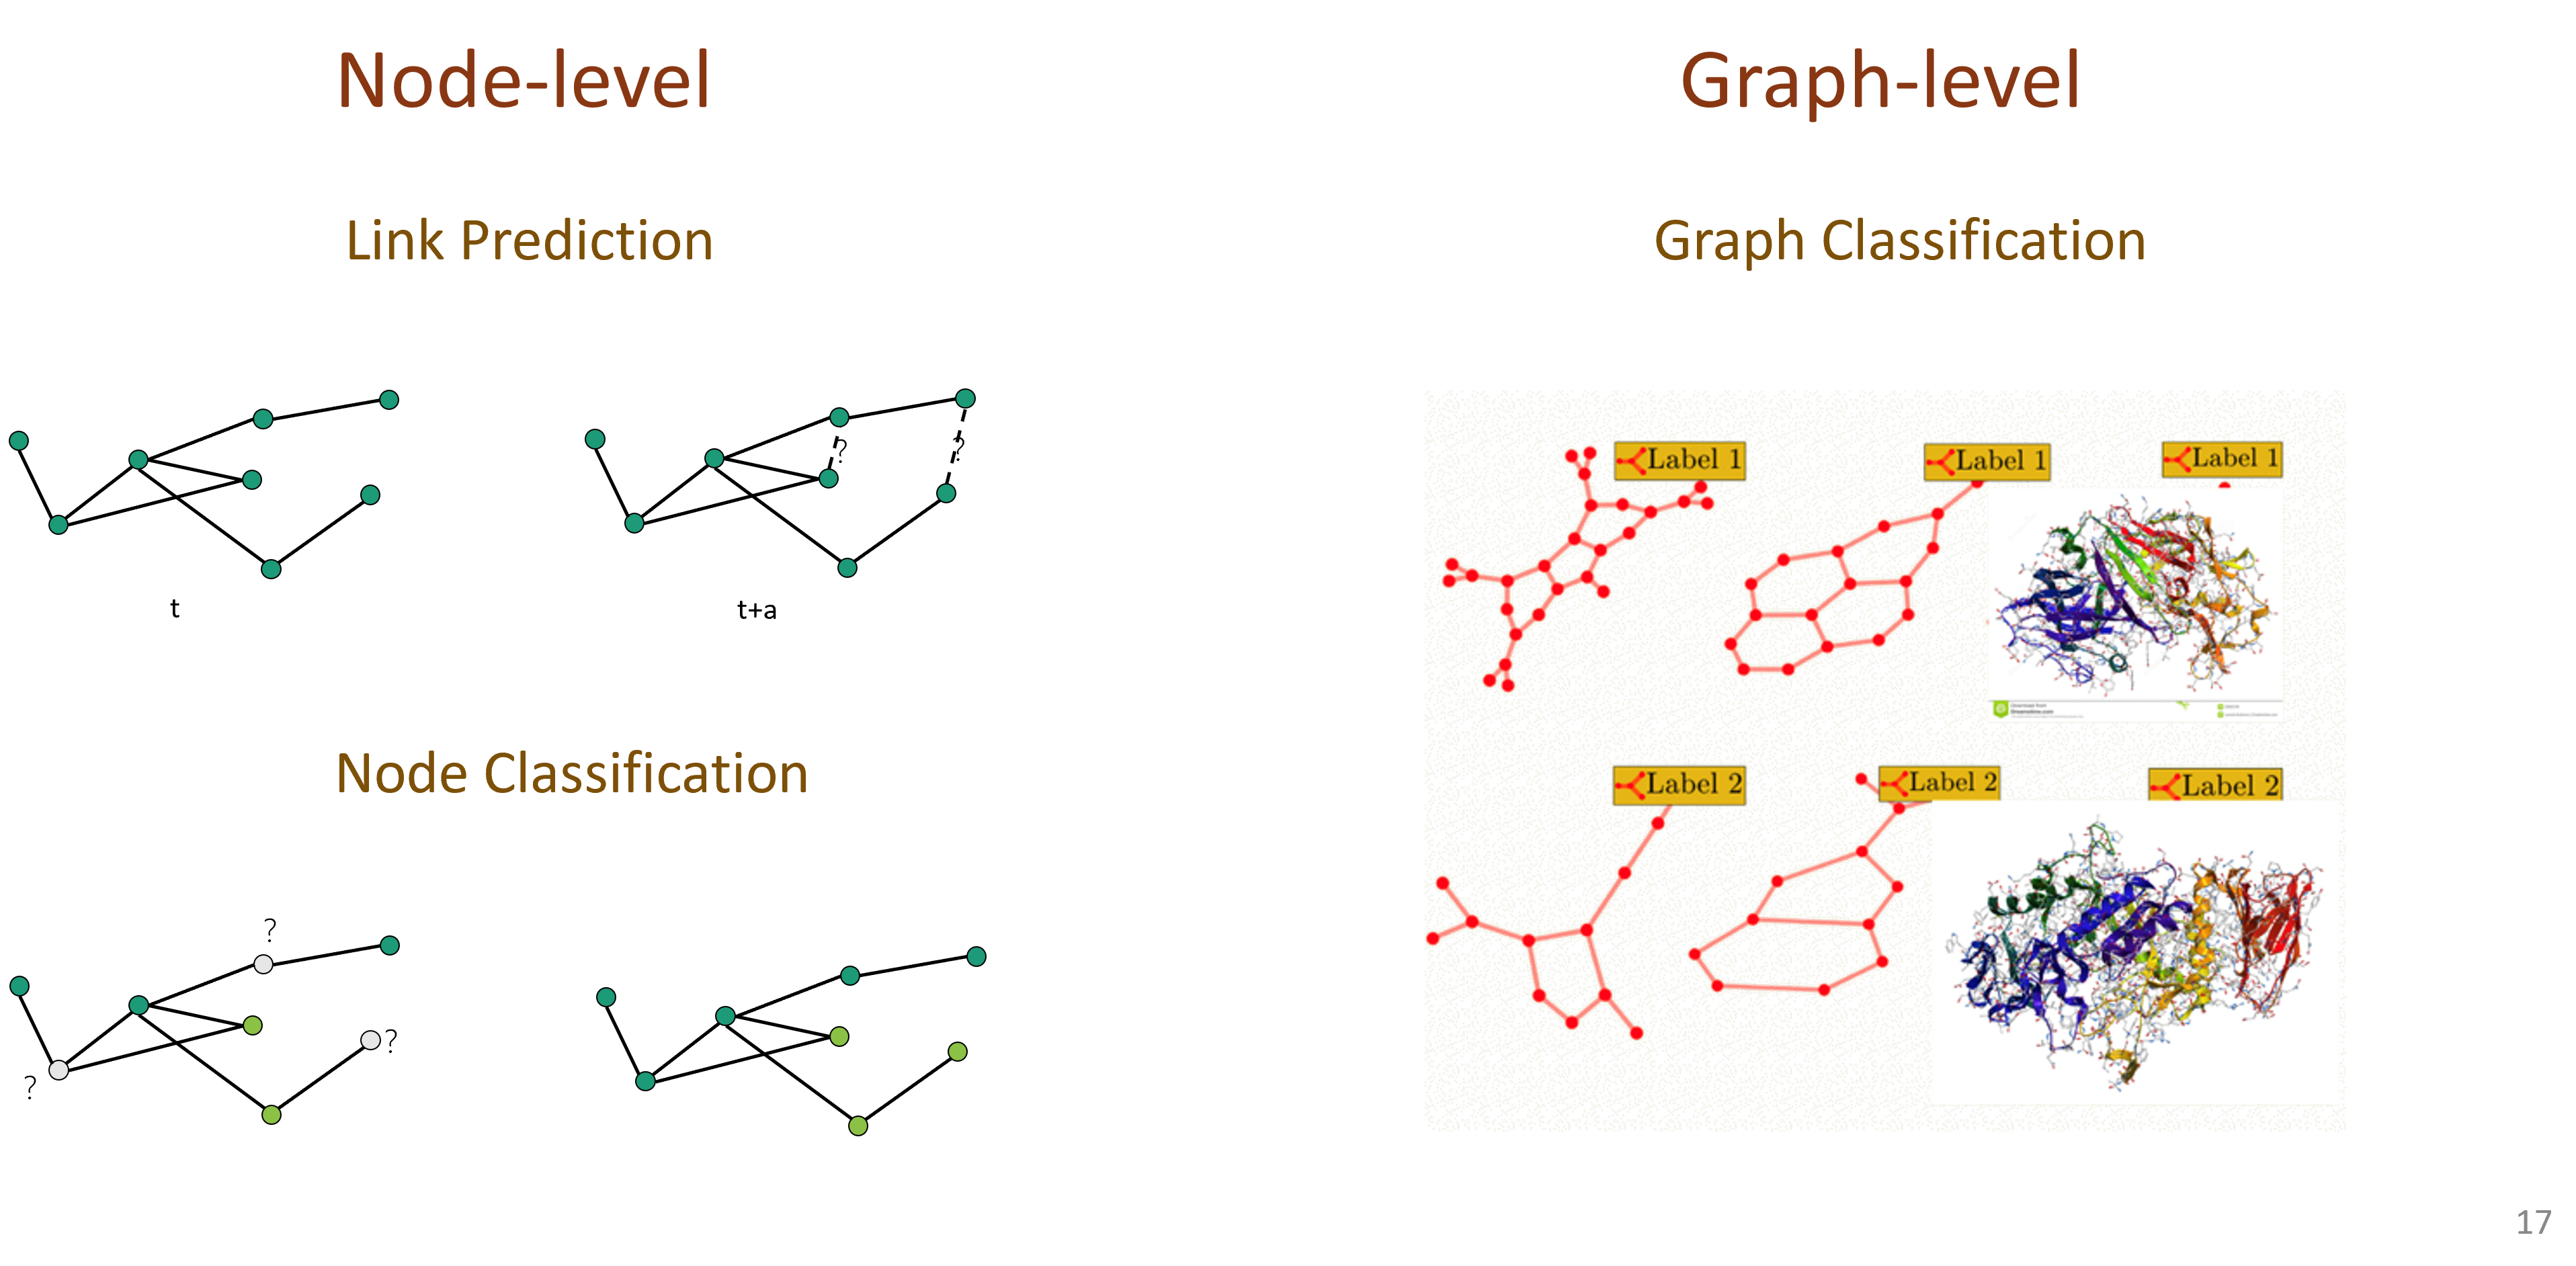
\includegraphics[width=\linewidth,keepaspectratio]{gnn14}
\end{center}	  

\end{frame}

%%%%%%%%%%%%%%%%%%%%%%%%%%%%%%%%%%%%%%%%%%%%%%%%%%%%%%%%%%%
\begin{frame}[fragile]\frametitle{ML on Graphs}
\begin{columns}
    \begin{column}[T]{0.6\linewidth}
		Numerous real-world problems can be summarized as a set of tasks on graphs

    \begin{itemize}
		\item Link prediction 
		\item Node Classification 
		\item Community Detection 
		\item Ranking \ldots
	  \end{itemize}

    \end{column}
    \begin{column}[T]{0.4\linewidth}
		ML solutions
		\begin{center}
		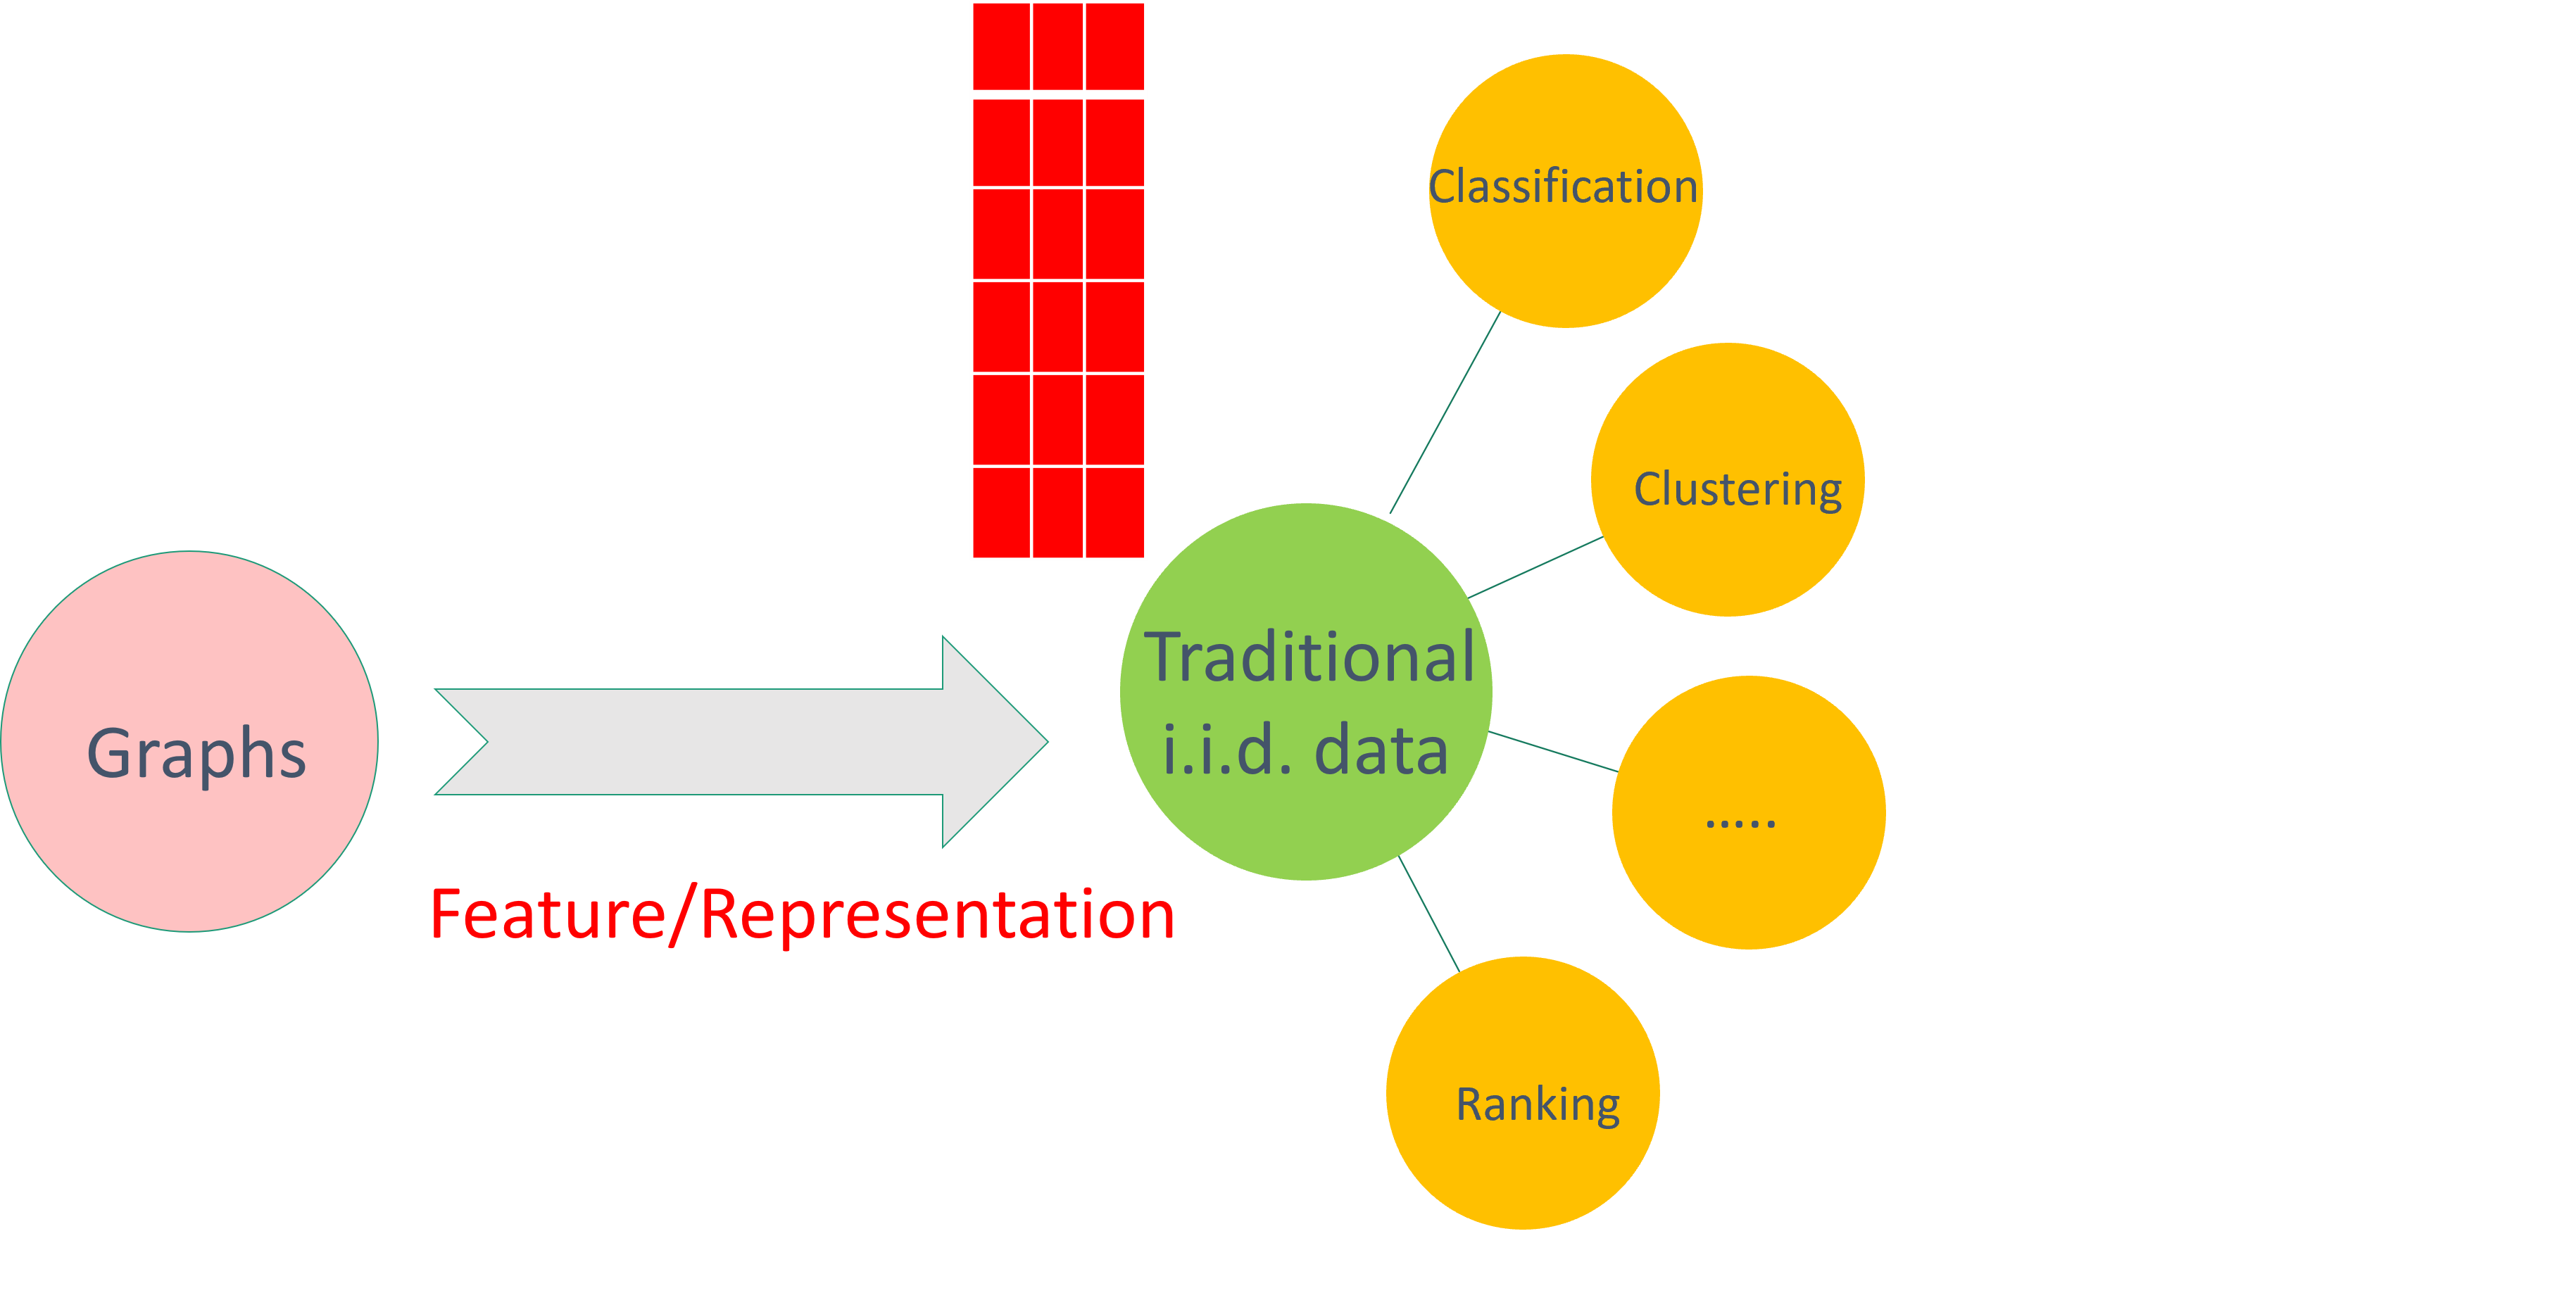
\includegraphics[width=\linewidth,keepaspectratio]{gnn15}
		\end{center}	 
    \end{column}
  \end{columns}
\end{frame}


%%%%%%%%%%%%%%%%%%%%%%%%%%%%%%%%%%%%%%%%%%%%%%%%%%%%%%%%%%%
\begin{frame}[fragile]\frametitle{}

\begin{center}
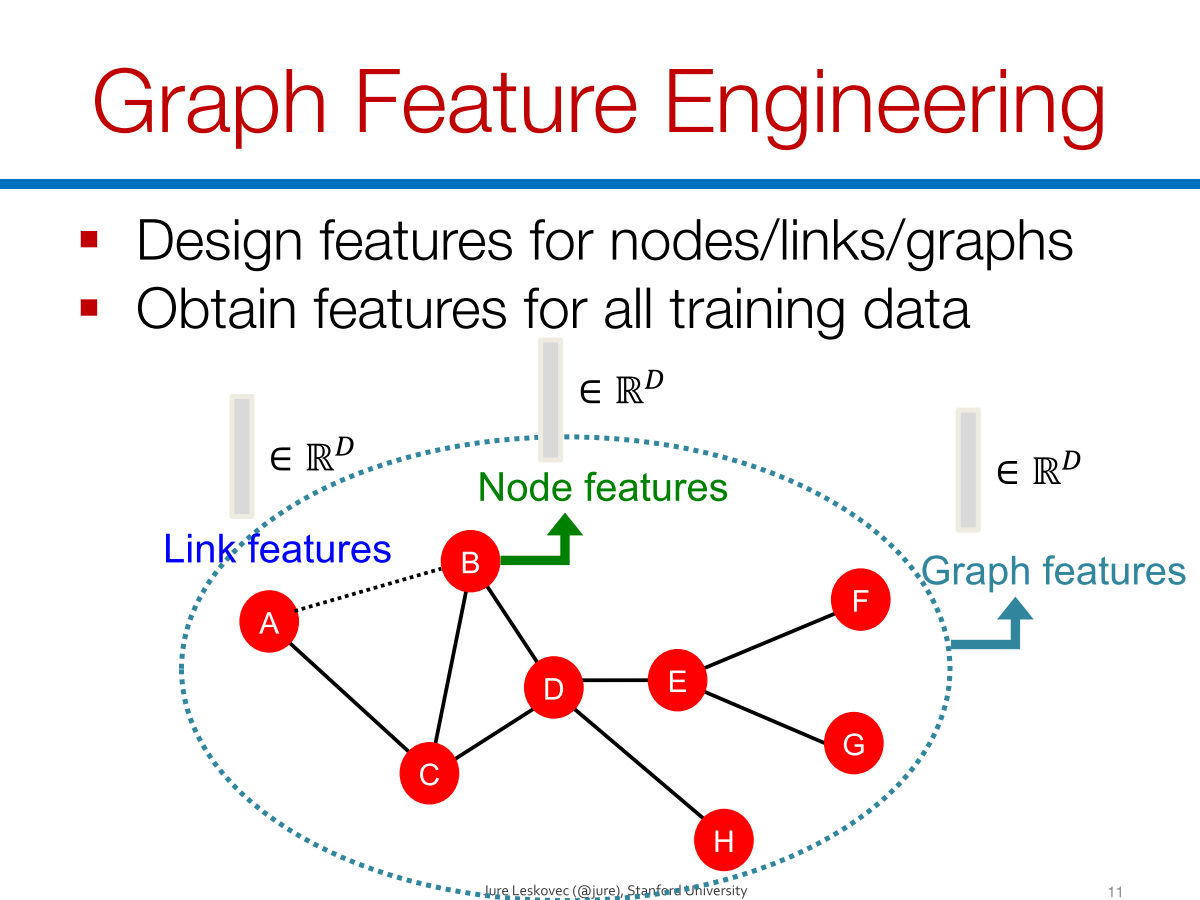
\includegraphics[width=\linewidth,keepaspectratio]{gnn16}
\end{center}	  

\end{frame}

%%%%%%%%%%%%%%%%%%%%%%%%%%%%%%%%%%%%%%%%%%%%%%%%%%%%%%%%%%%
\begin{frame}[fragile]\frametitle{}

\begin{center}
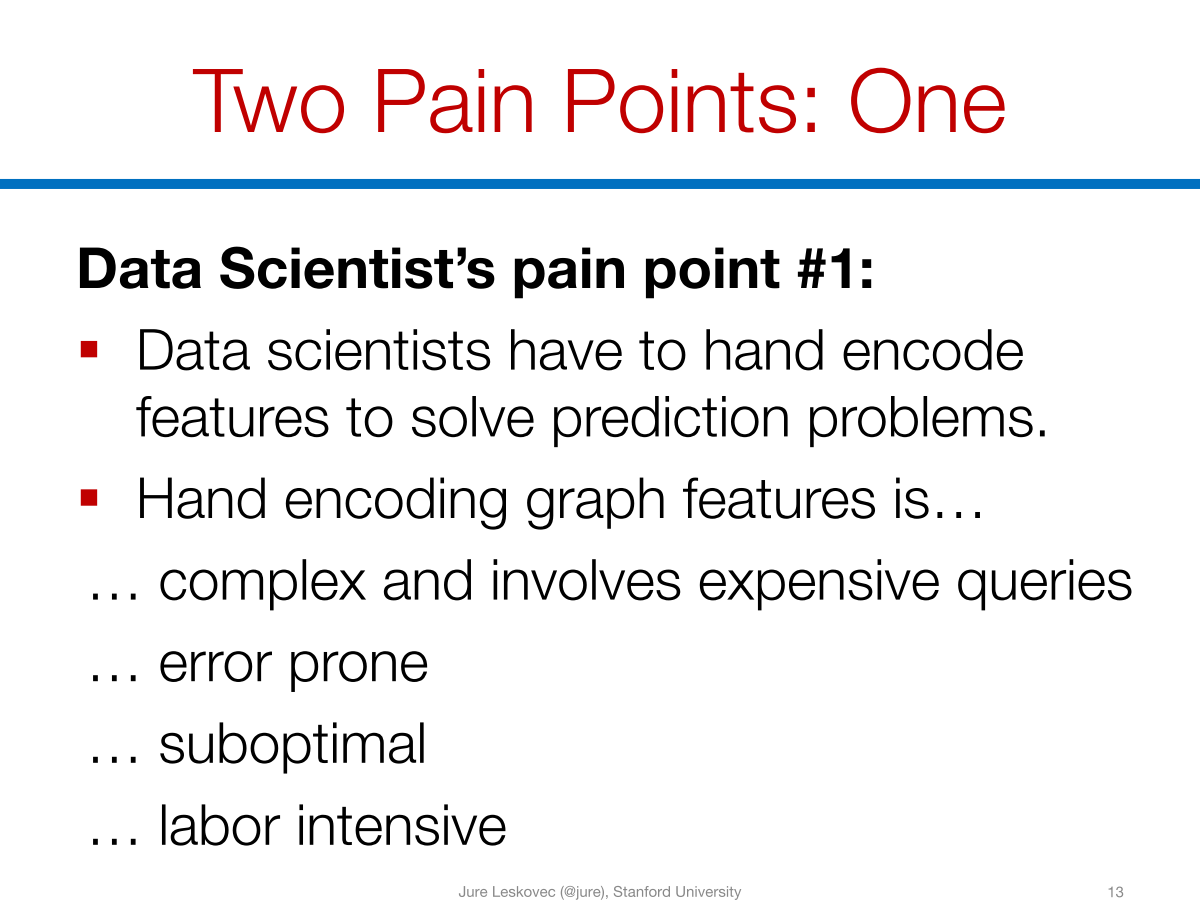
\includegraphics[width=\linewidth,keepaspectratio]{gnn17}
\end{center}	  

\end{frame}

%%%%%%%%%%%%%%%%%%%%%%%%%%%%%%%%%%%%%%%%%%%%%%%%%%%%%%%%%%%
\begin{frame}[fragile]\frametitle{}

\begin{center}
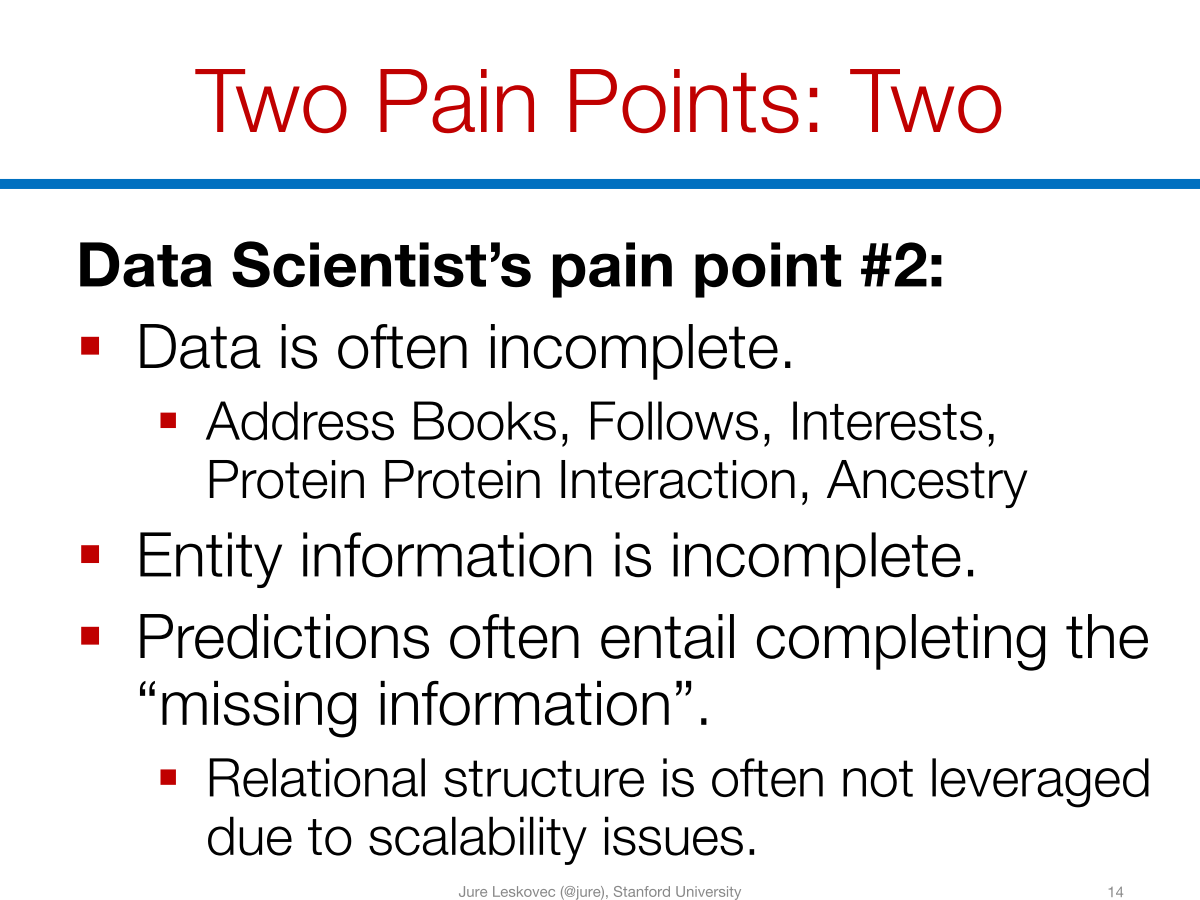
\includegraphics[width=\linewidth,keepaspectratio]{gnn18}
\end{center}	  

\end{frame}

%%%%%%%%%%%%%%%%%%%%%%%%%%%%%%%%%%%%%%%%%%%%%%%%%%%%%%%%%%%
\begin{frame}[fragile]\frametitle{}

\begin{center}
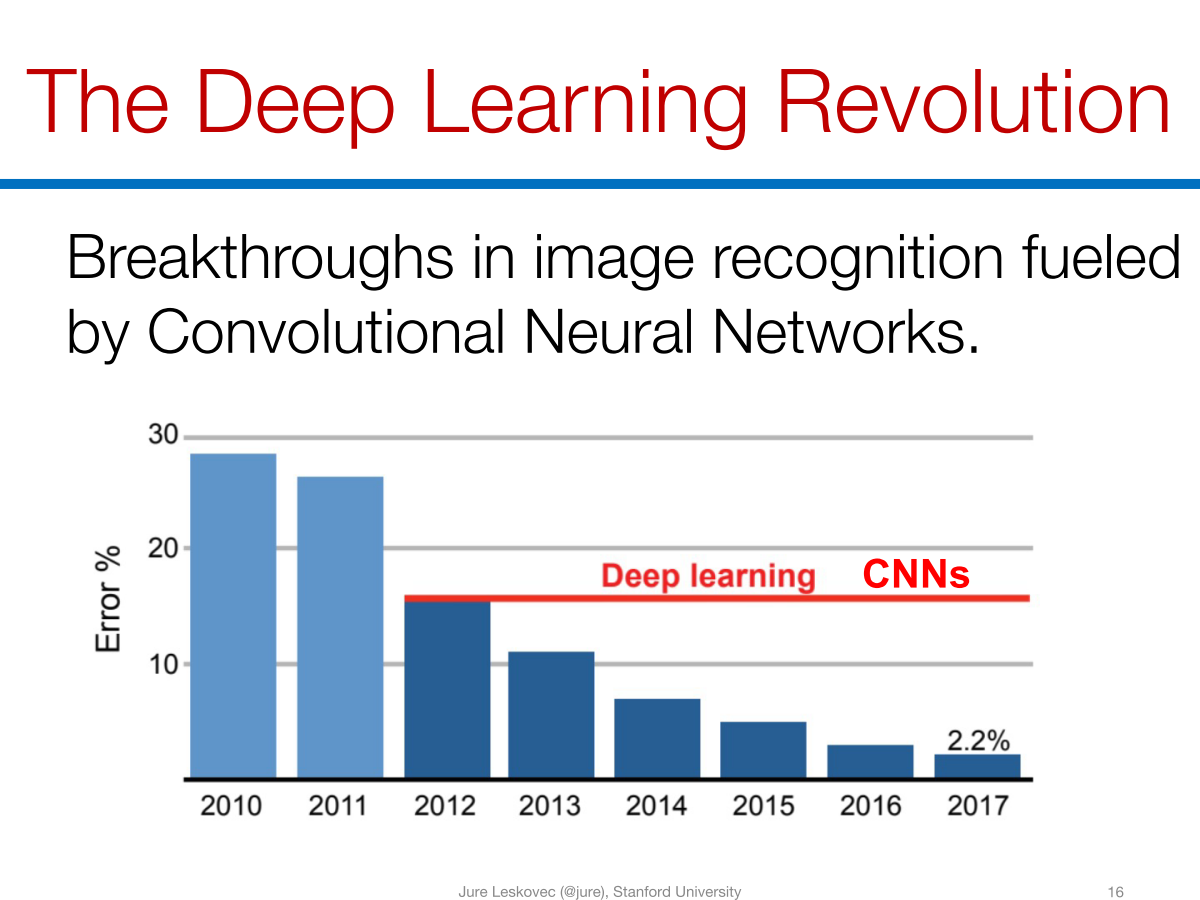
\includegraphics[width=\linewidth,keepaspectratio]{gnn19}
\end{center}	  

\end{frame}

%%%%%%%%%%%%%%%%%%%%%%%%%%%%%%%%%%%%%%%%%%%%%%%%%%%%%%%%%%%
\begin{frame}[fragile]\frametitle{}

\begin{center}
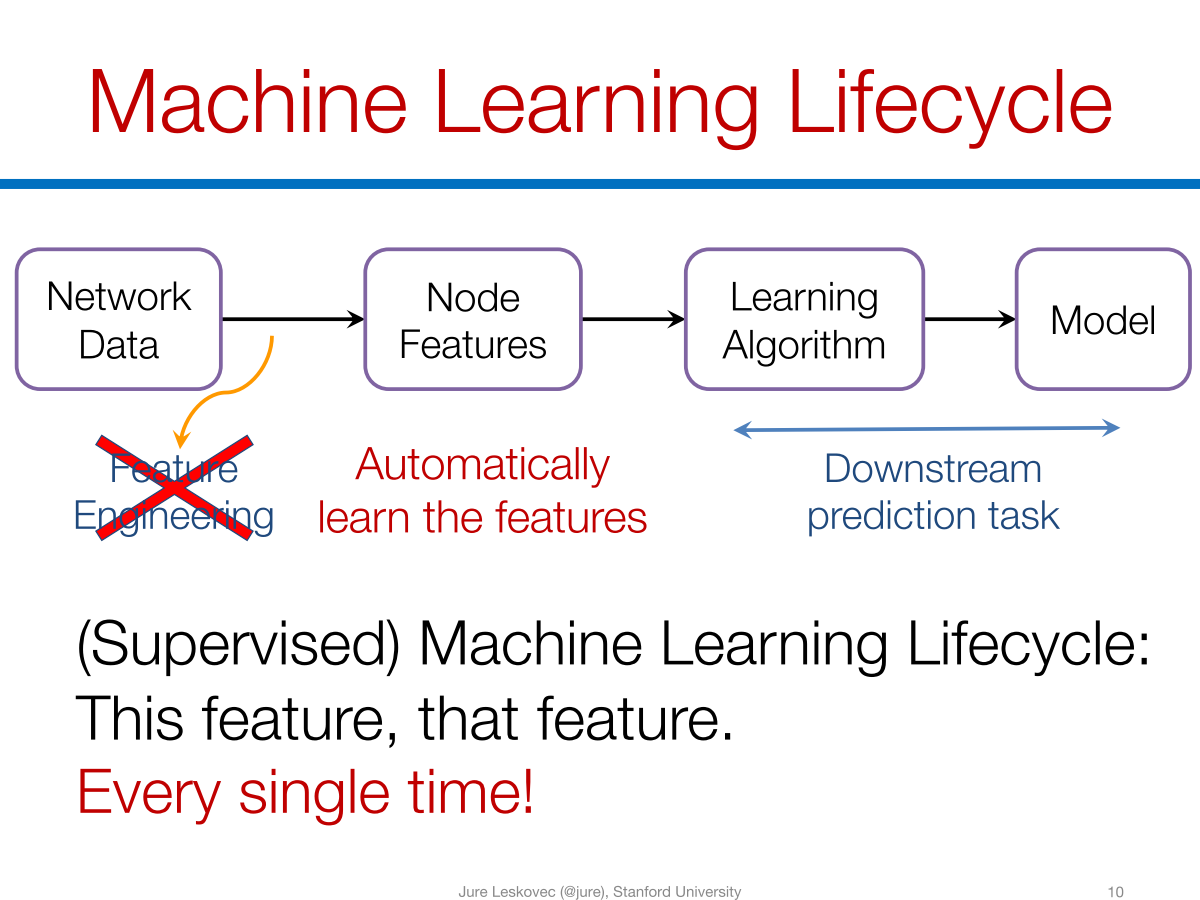
\includegraphics[width=\linewidth,keepaspectratio]{gnn20}
\end{center}	  

\end{frame}

%%%%%%%%%%%%%%%%%%%%%%%%%%%%%%%%%%%%%%%%%%%%%%%%%%%%%%%%%%%
\begin{frame}[fragile]\frametitle{}

\begin{center}
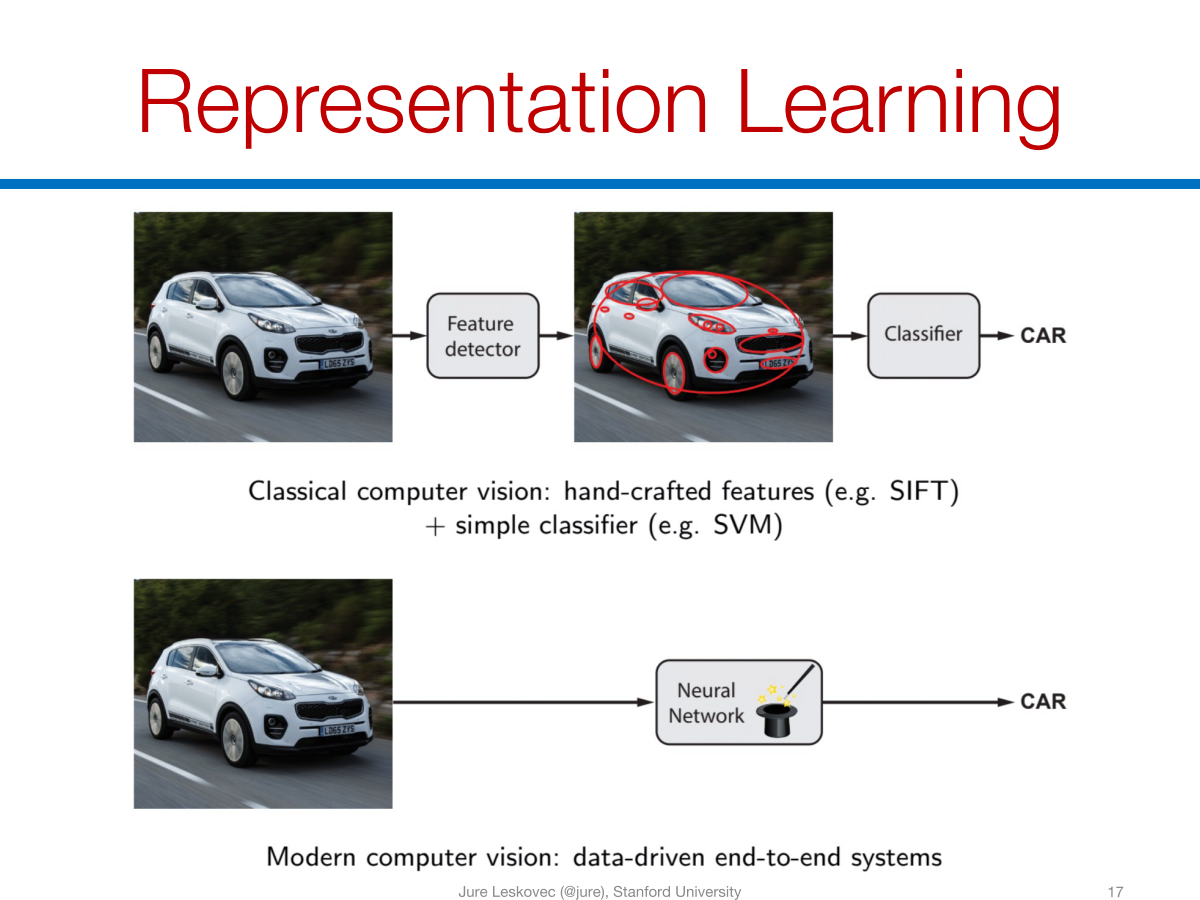
\includegraphics[width=\linewidth,keepaspectratio]{gnn21}
\end{center}	  

\end{frame}

%%%%%%%%%%%%%%%%%%%%%%%%%%%%%%%%%%%%%%%%%%%%%%%%%%%%%%%%%%%
\begin{frame}[fragile]\frametitle{}

\begin{center}
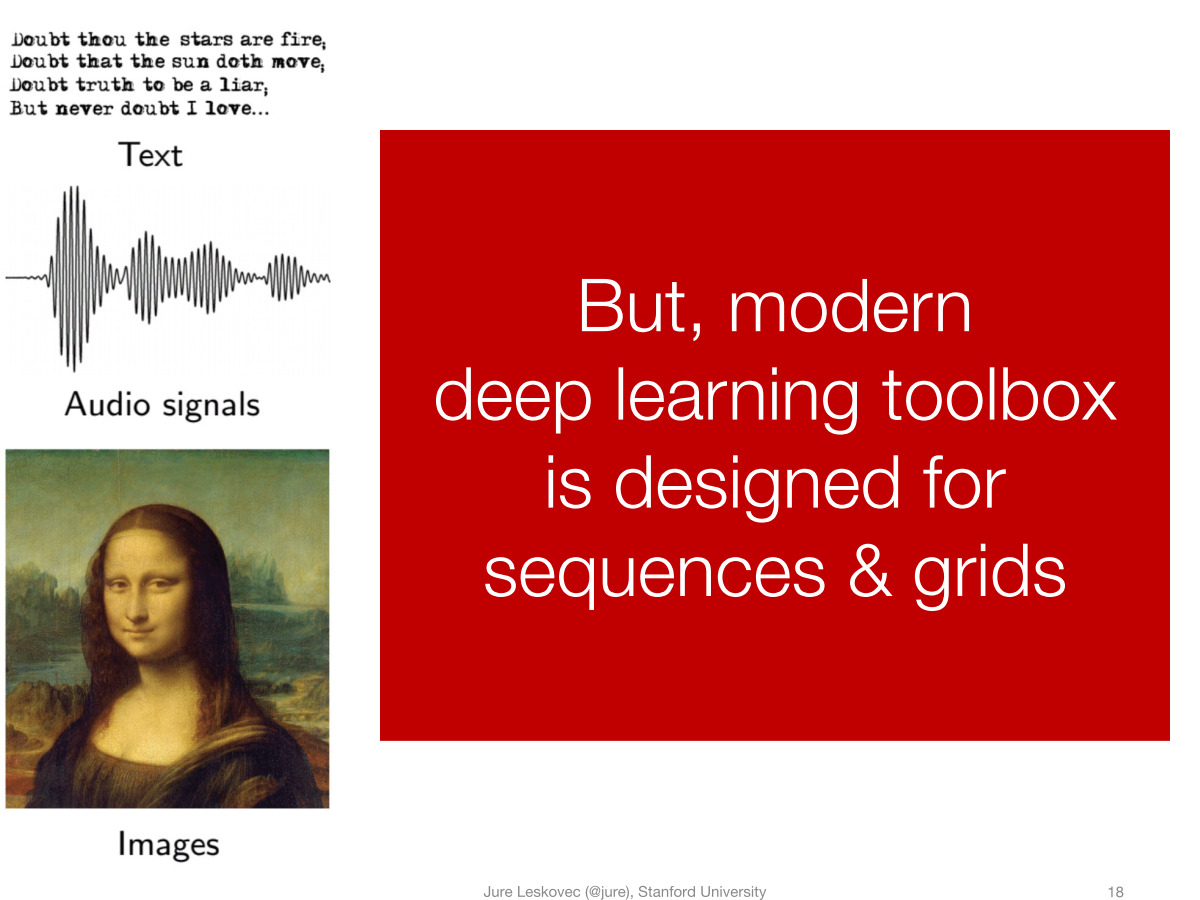
\includegraphics[width=\linewidth,keepaspectratio]{gnn22}
\end{center}	  

\end{frame}

%%%%%%%%%%%%%%%%%%%%%%%%%%%%%%%%%%%%%%%%%%%%%%%%%%%%%%%%%%%
\begin{frame}[fragile]\frametitle{}

\begin{center}
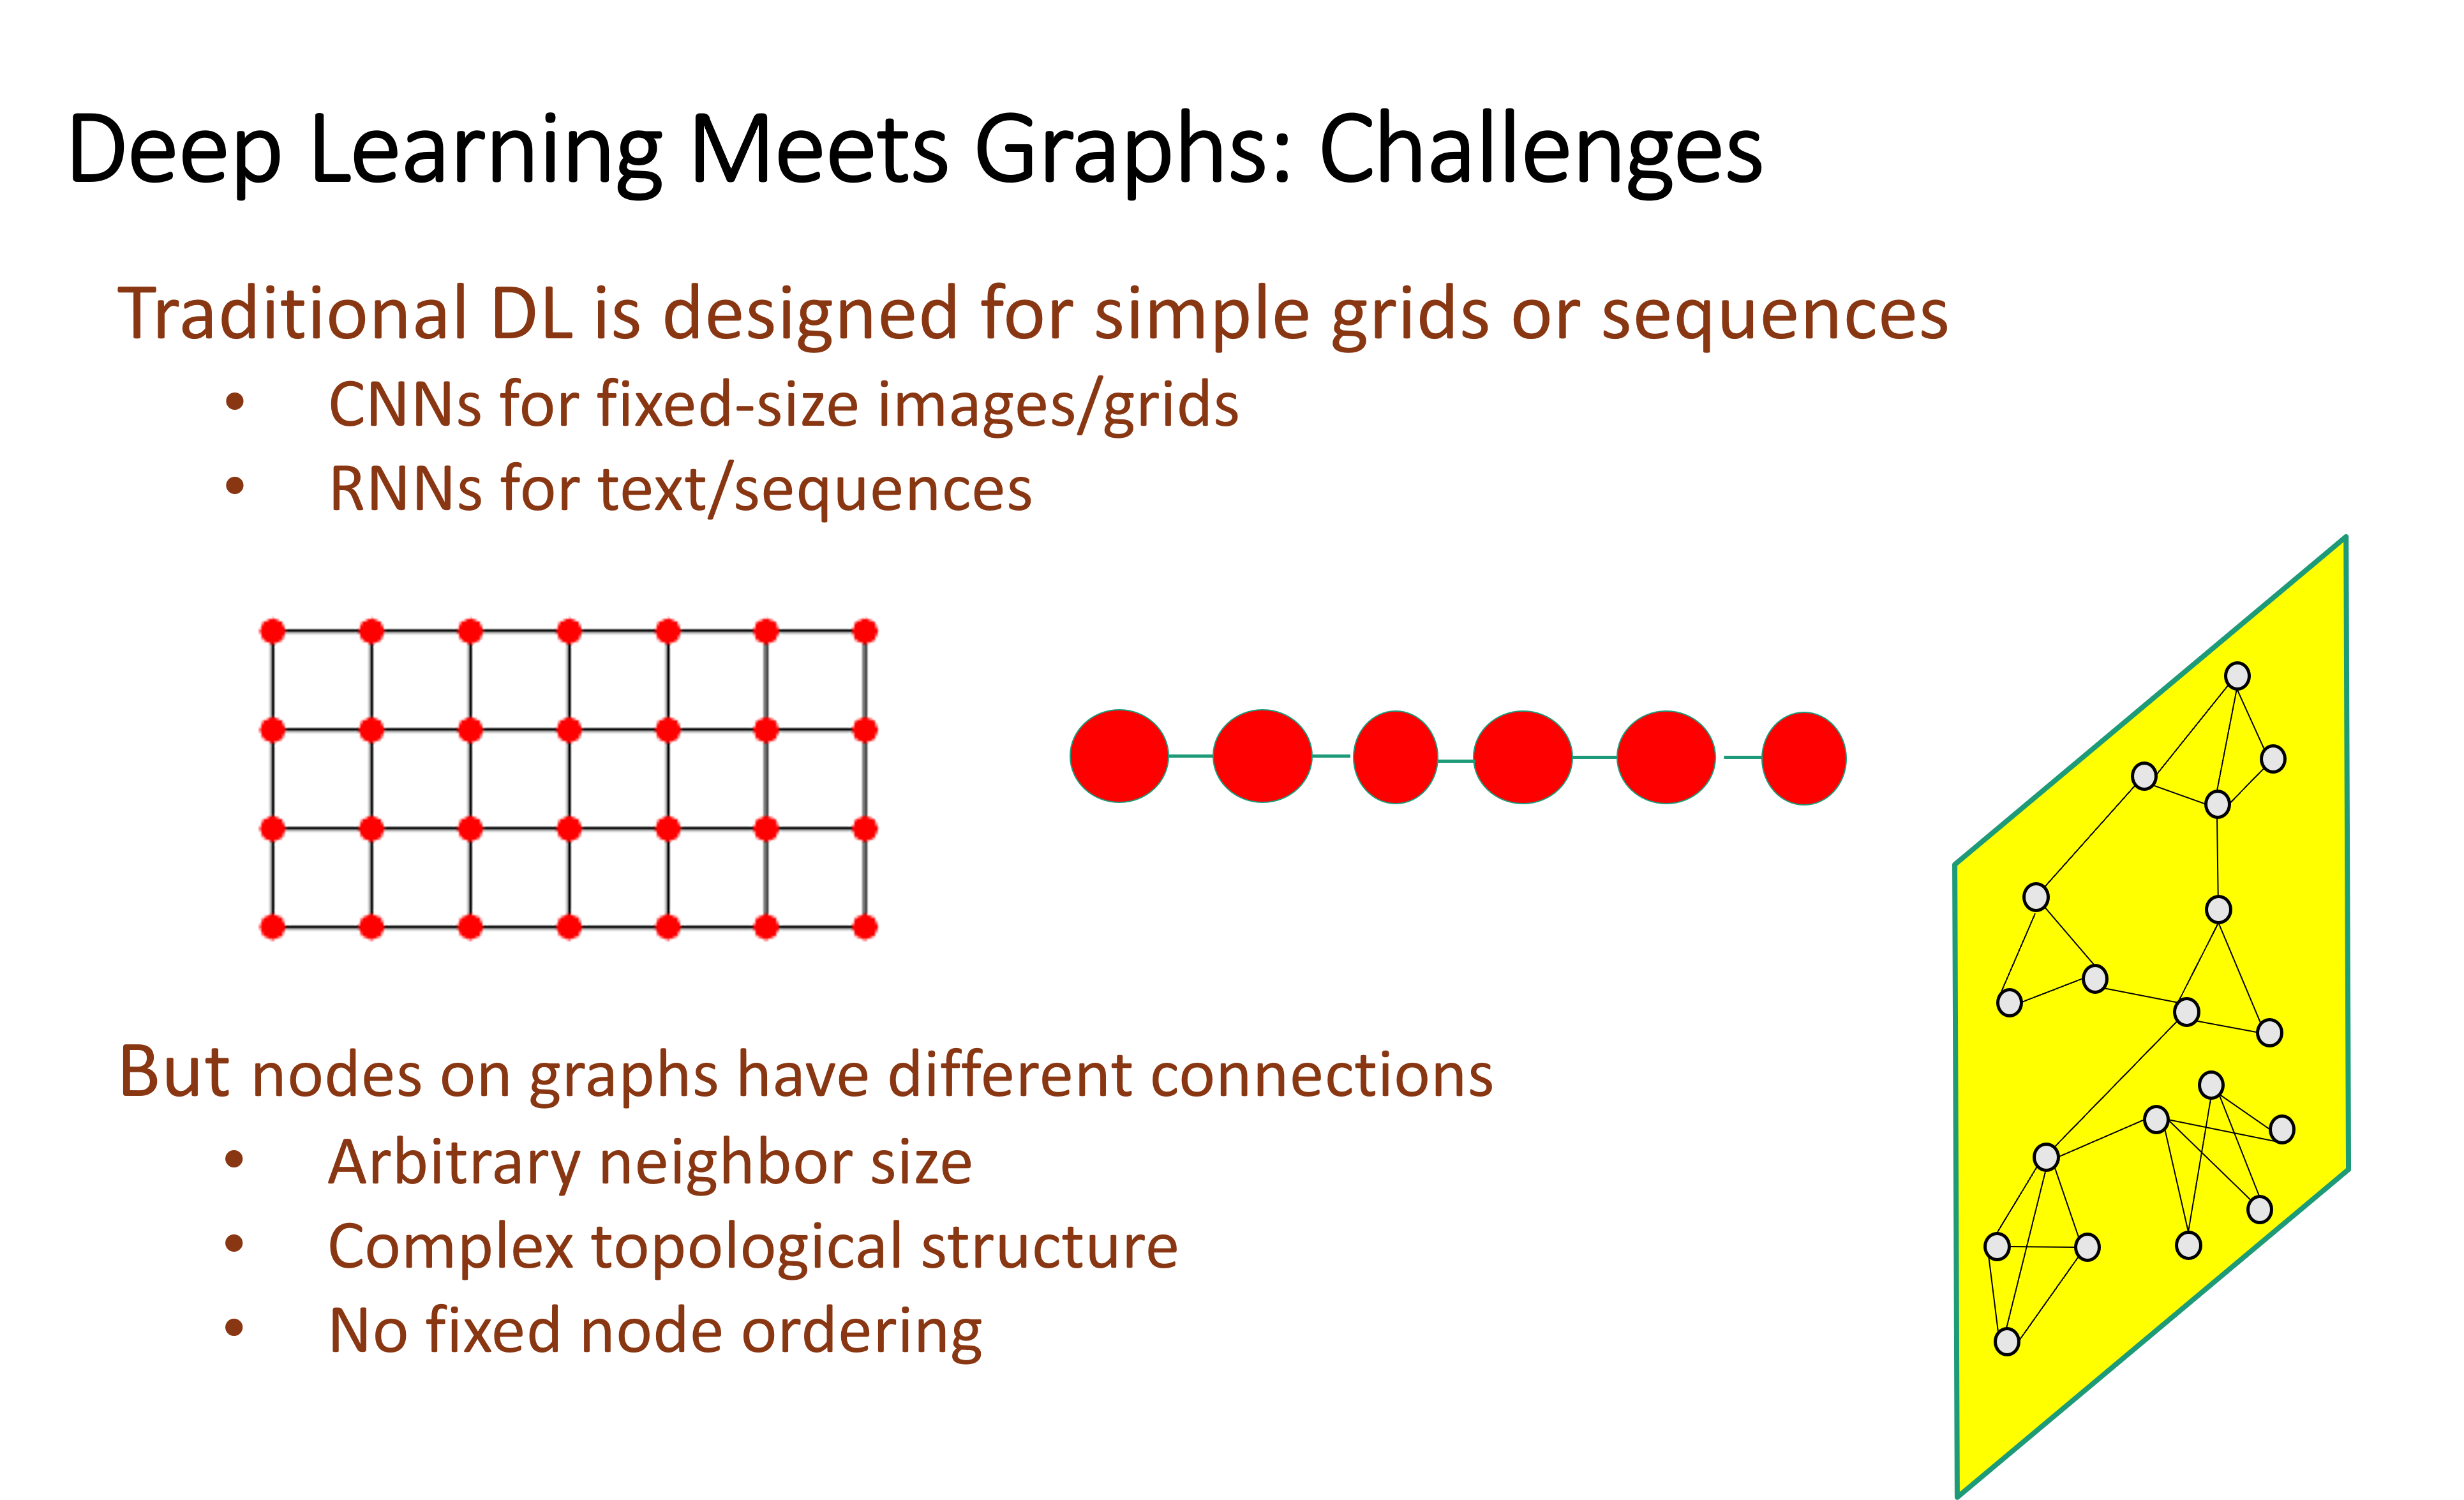
\includegraphics[width=\linewidth,keepaspectratio]{gnn23}
\end{center}	  

\end{frame}

%%%%%%%%%%%%%%%%%%%%%%%%%%%%%%%%%%%%%%%%%%%%%%%%%%%%%%%%%%%
\begin{frame}[fragile]\frametitle{}

\begin{center}
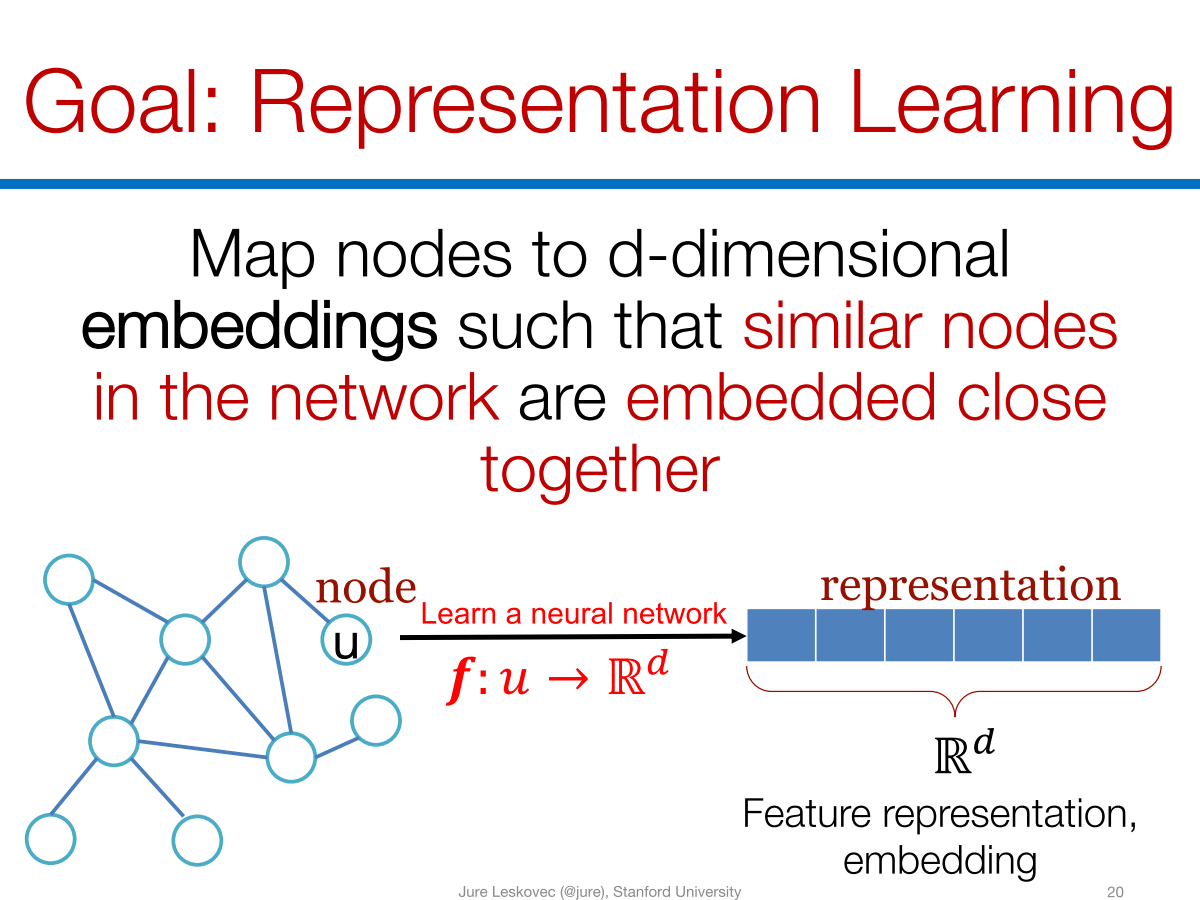
\includegraphics[width=\linewidth,keepaspectratio]{gnn24}
\end{center}	  

\end{frame}

%%%%%%%%%%%%%%%%%%%%%%%%%%%%%%%%%%%%%%%%%%%%%%%%%%%%%%%%%%%
\begin{frame}[fragile]\frametitle{The Power of Deep Learning}

\begin{center}
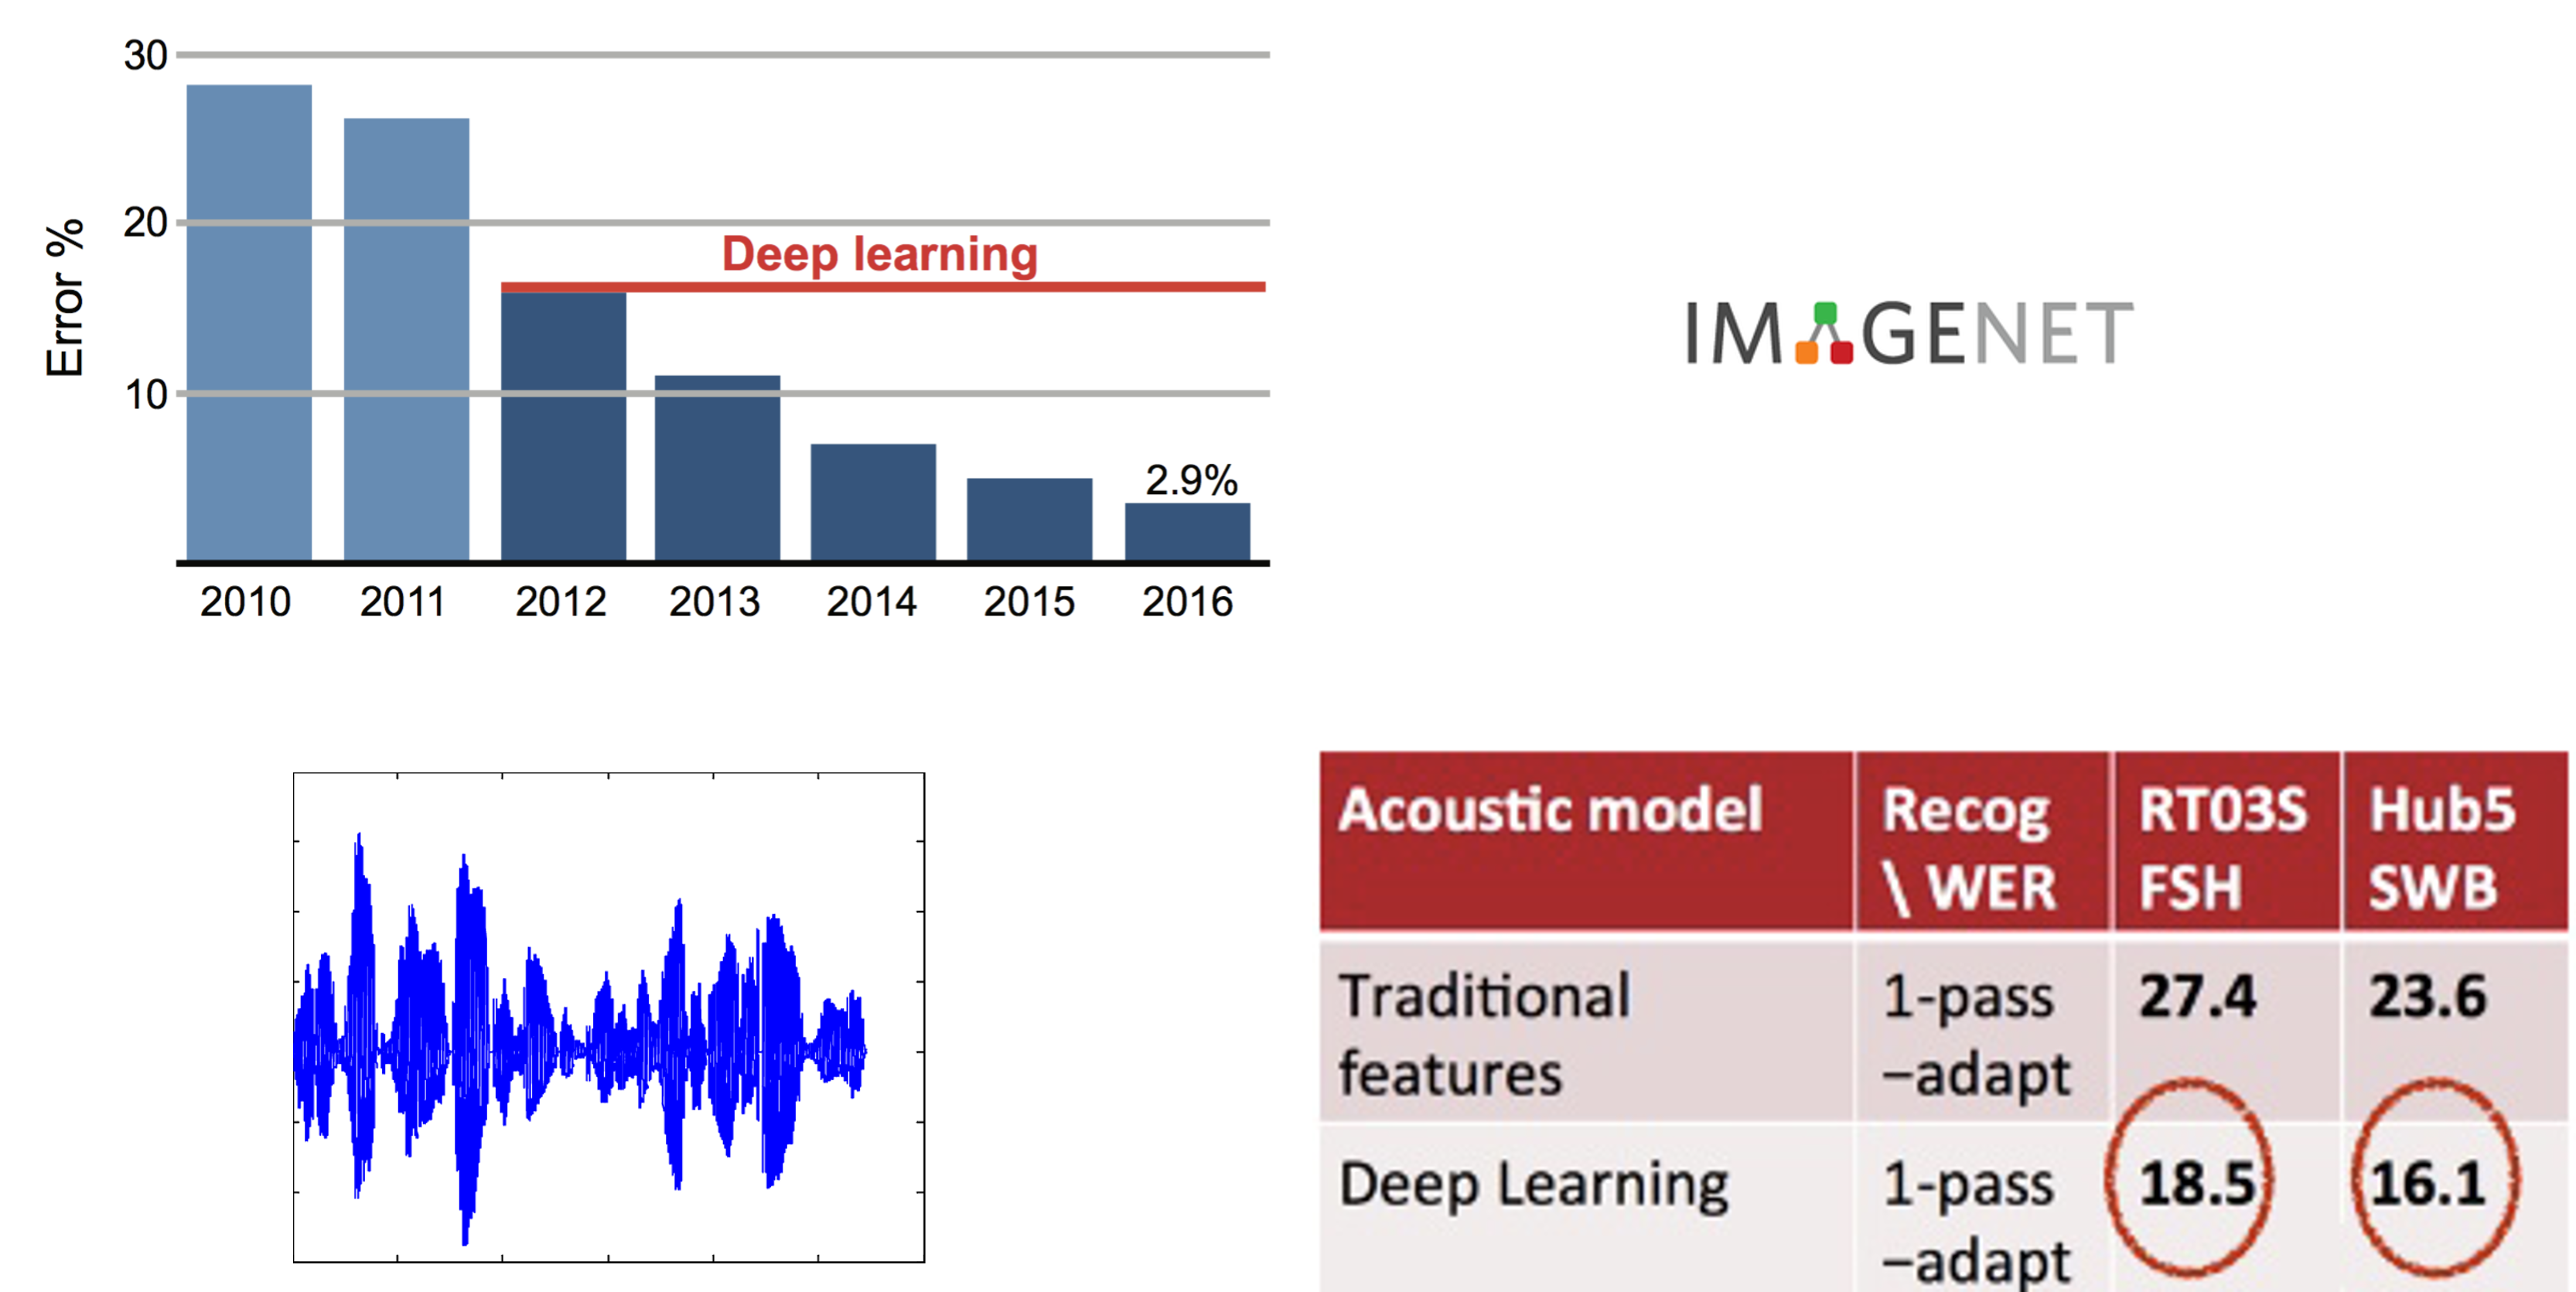
\includegraphics[width=\linewidth,keepaspectratio]{gnn25}
\end{center}	  

\end{frame}

%%%%%%%%%%%%%%%%%%%%%%%%%%%%%%%%%%%%%%%%%%%%%%%%%%%%%%%%%%%
\begin{frame}[fragile]\frametitle{}

\begin{center}
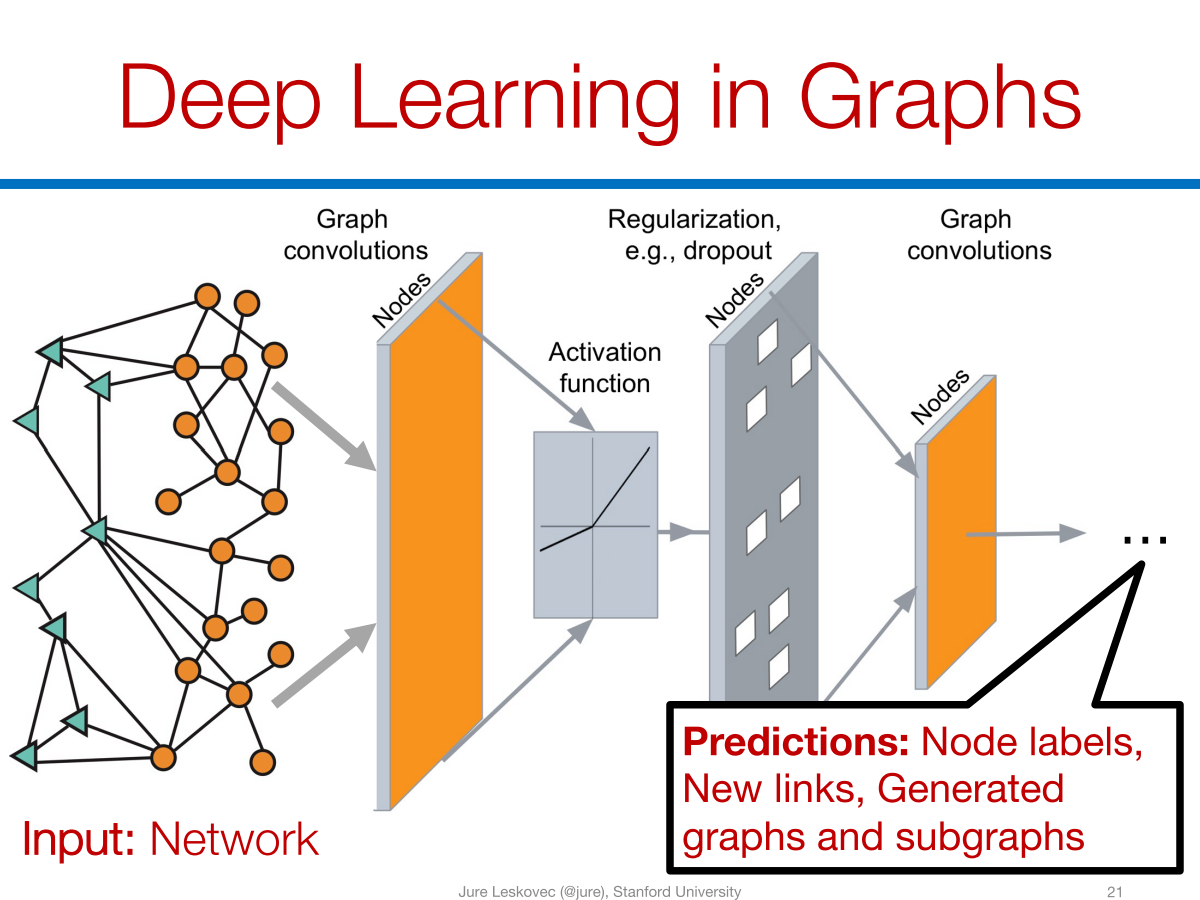
\includegraphics[width=\linewidth,keepaspectratio]{gnn26}
\end{center}	  

\end{frame}

%%%%%%%%%%%%%%%%%%%%%%%%%%%%%%%%%%%%%%%%%%%%%%%%%%%%%%%%%%%
\begin{frame}[fragile]\frametitle{}

\begin{center}
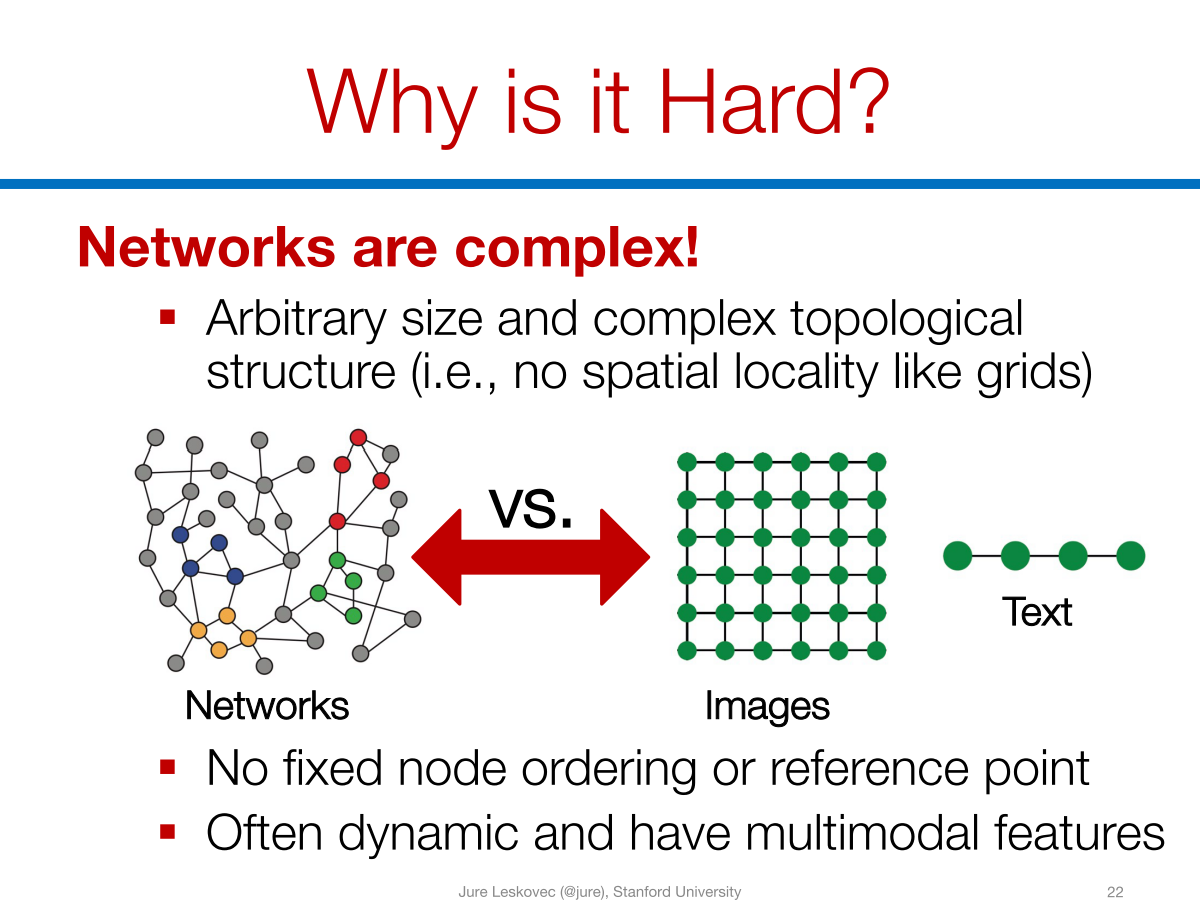
\includegraphics[width=\linewidth,keepaspectratio]{gnn27}
\end{center}	  

\end{frame}

%%%%%%%%%%%%%%%%%%%%%%%%%%%%%%%%%%%%%%%%%%%%%%%%%%%%%%%%%%%
\begin{frame}[fragile]\frametitle{}

\begin{center}
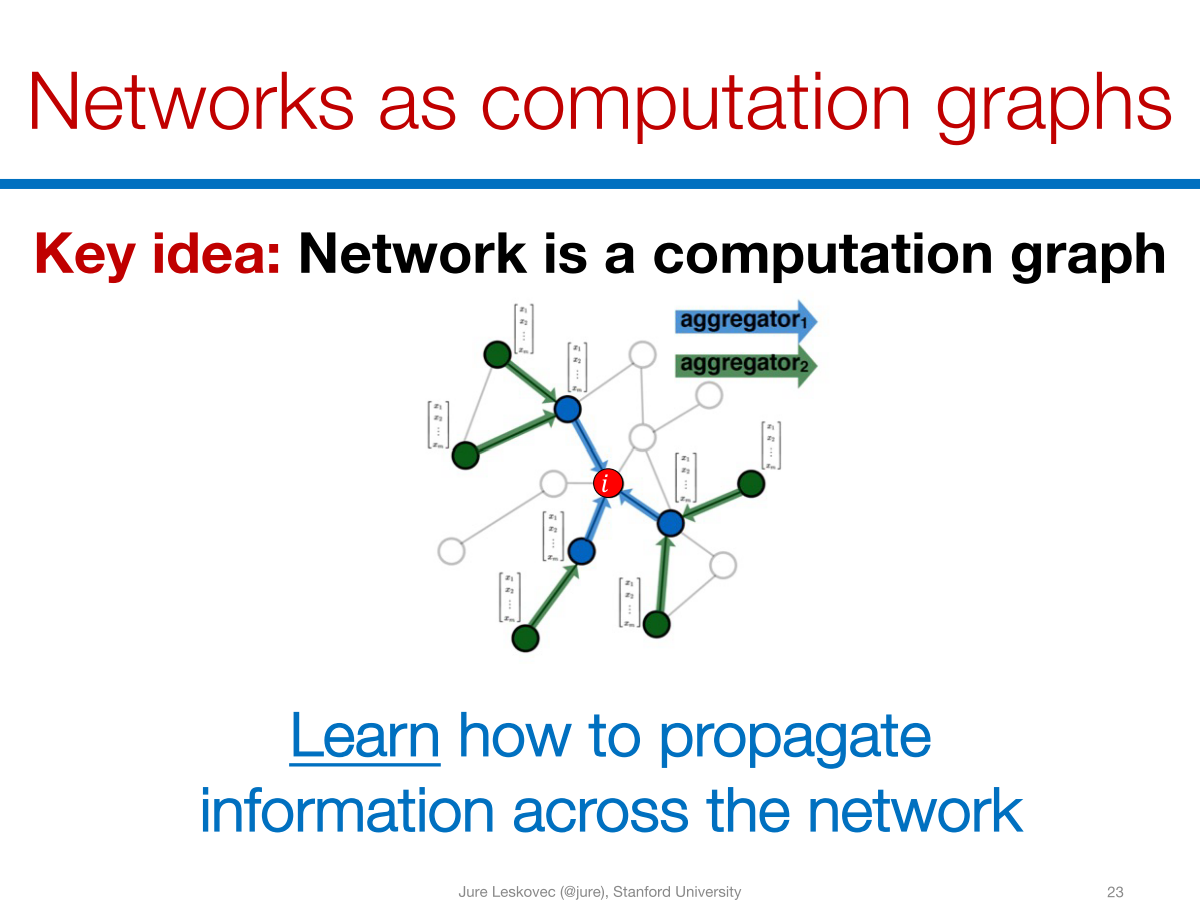
\includegraphics[width=\linewidth,keepaspectratio]{gnn28}
\end{center}	  

\end{frame}

%%%%%%%%%%%%%%%%%%%%%%%%%%%%%%%%%%%%%%%%%%%%%%%%%%%%%%%%%%%
\begin{frame}[fragile]\frametitle{Graph Neural Networks}

\begin{center}
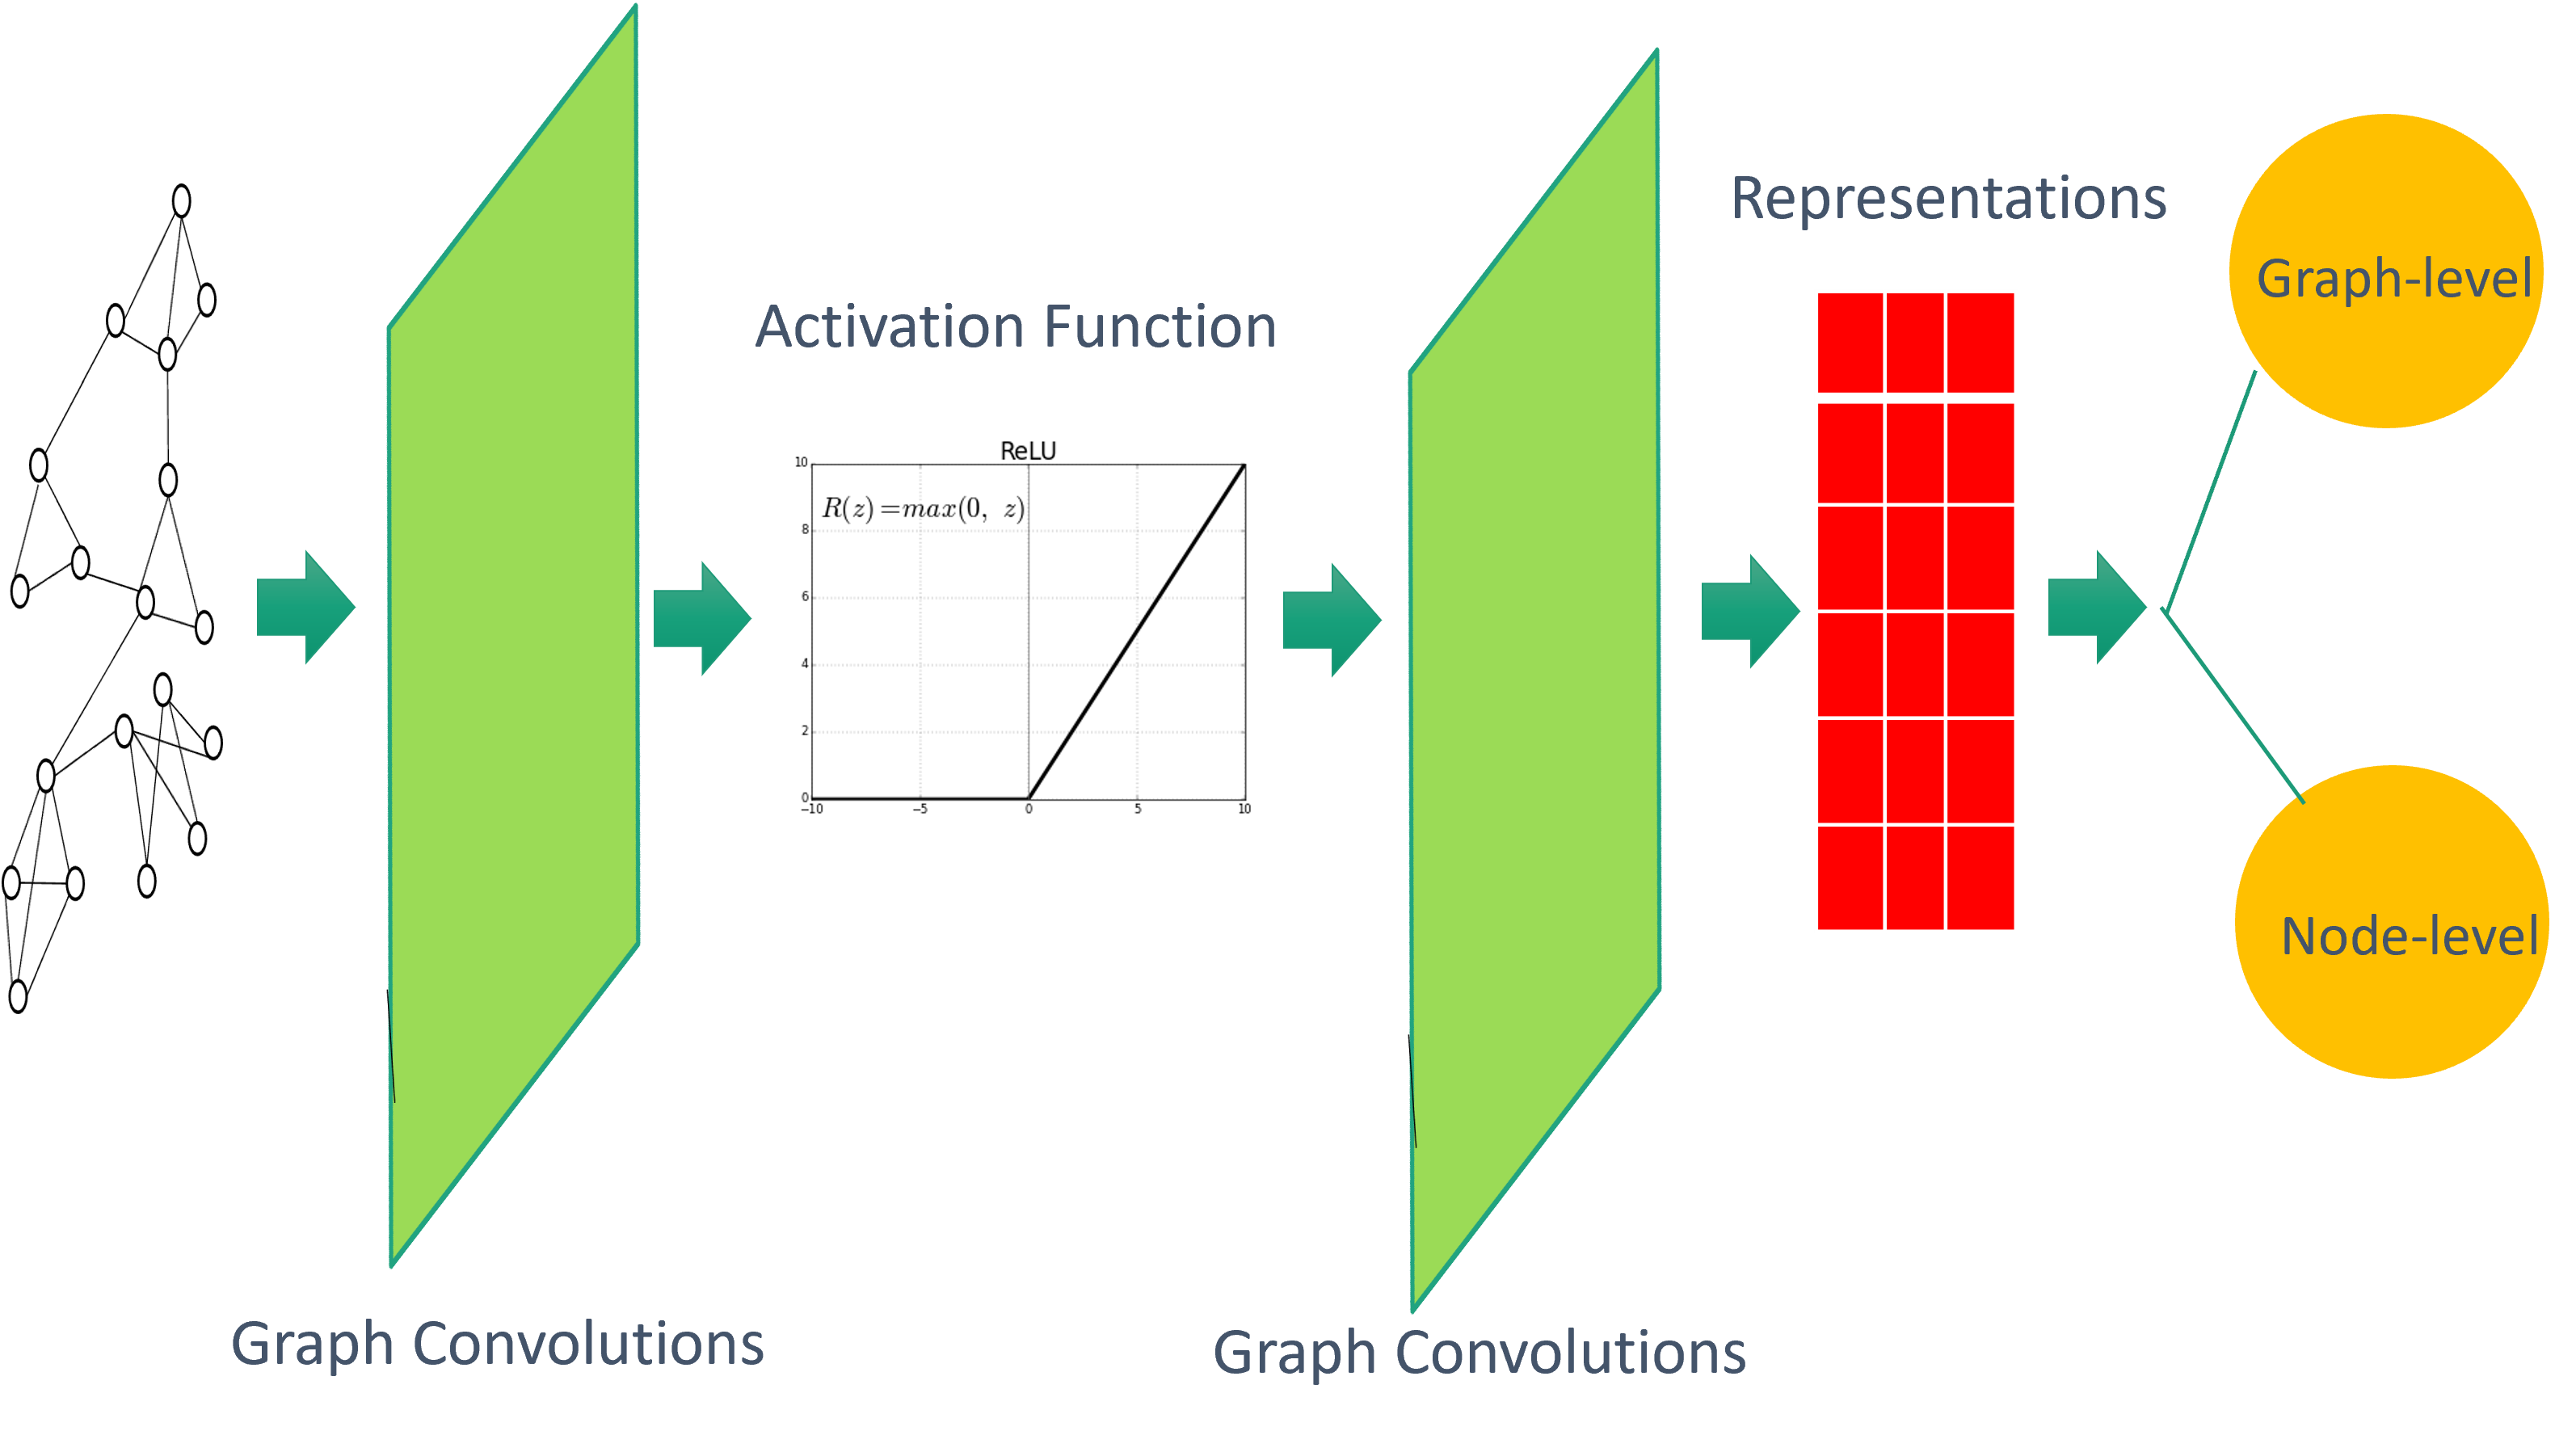
\includegraphics[width=\linewidth,keepaspectratio]{gnn29}
\end{center}	  

\end{frame}

%%%%%%%%%%%%%%%%%%%%%%%%%%%%%%%%%%%%%%%%%%%%%%%%%%%%%%%%%%%
\begin{frame}[fragile]\frametitle{Machine(Deep) Learning with Graphs}
\begin{columns}
    \begin{column}[T]{0.6\linewidth}
		Classical ML tasks in graphs:

    \begin{itemize}
		\item Node classification: Predict a type of a given node
		\item Link prediction: Predict whether two nodes are linked
		\item Community detection: Identify densely linked clusters of nodes
		\item Graph similarity: How similar are two (sub)graphs
	  \end{itemize}

    \end{column}
    \begin{column}[T]{0.4\linewidth}
		Recent ML tasks in graphs:
		
    \begin{itemize}
		\item Graph classification: Predict a type of a given graph
		\item Graph generation: Generate graphs from learned distribution
		\item Graph structure learning : Identify densely linked clusters of nodes
		\item Graph-to-XXX learning: Graph Inputs – XXX outputs
	  \end{itemize} 
		
    \end{column}
  \end{columns}
\end{frame}

%%%%%%%%%%%%%%%%%%%%%%%%%%%%%%%%%%%%%%%%%%%%%%%%%%%%%%%%%%%
\begin{frame}[fragile]\frametitle{Graph Representation Learning (GNNs)}

\begin{itemize}
		\item Graph Neural Networks (GNNs) extends the well known CNN and RNN on graphs, from Euclidean data to Graphs and Manifolds
		\item RNN-based GNNs: 
		\begin{itemize}
		\item Graph neural networks (Scarselli et al., 2009)
		\item Gated graph sequence neural networks (GGS-NNs) (Li et al., ICLR 2016)
		\end{itemize}

		\item CNN-based GNNs: 
		\begin{itemize}
 		\item Graph Convolutional Networks (GCN) (Kipf \& Welling, ICLR 2017)
		\end{itemize}

		\item Message Passing-based GNNs:
		\begin{itemize}
 		\item GraphSAGE (Hamilton \& Ying \& Leskovec, NIPS 2017)
 		\item Graph Attention Networks (GAT) (Velickovic et al., ICLR 2018) 
 		\item MPNN (Gilmer et al., ICML 2017)
		\end{itemize}

\end{itemize}

\end{frame}

%%%%%%%%%%%%%%%%%%%%%%%%%%%%%%%%%%%%%%%%%%%%%%%%%%%%%%%%%%%
\begin{frame}[fragile]\frametitle{}

\begin{center}
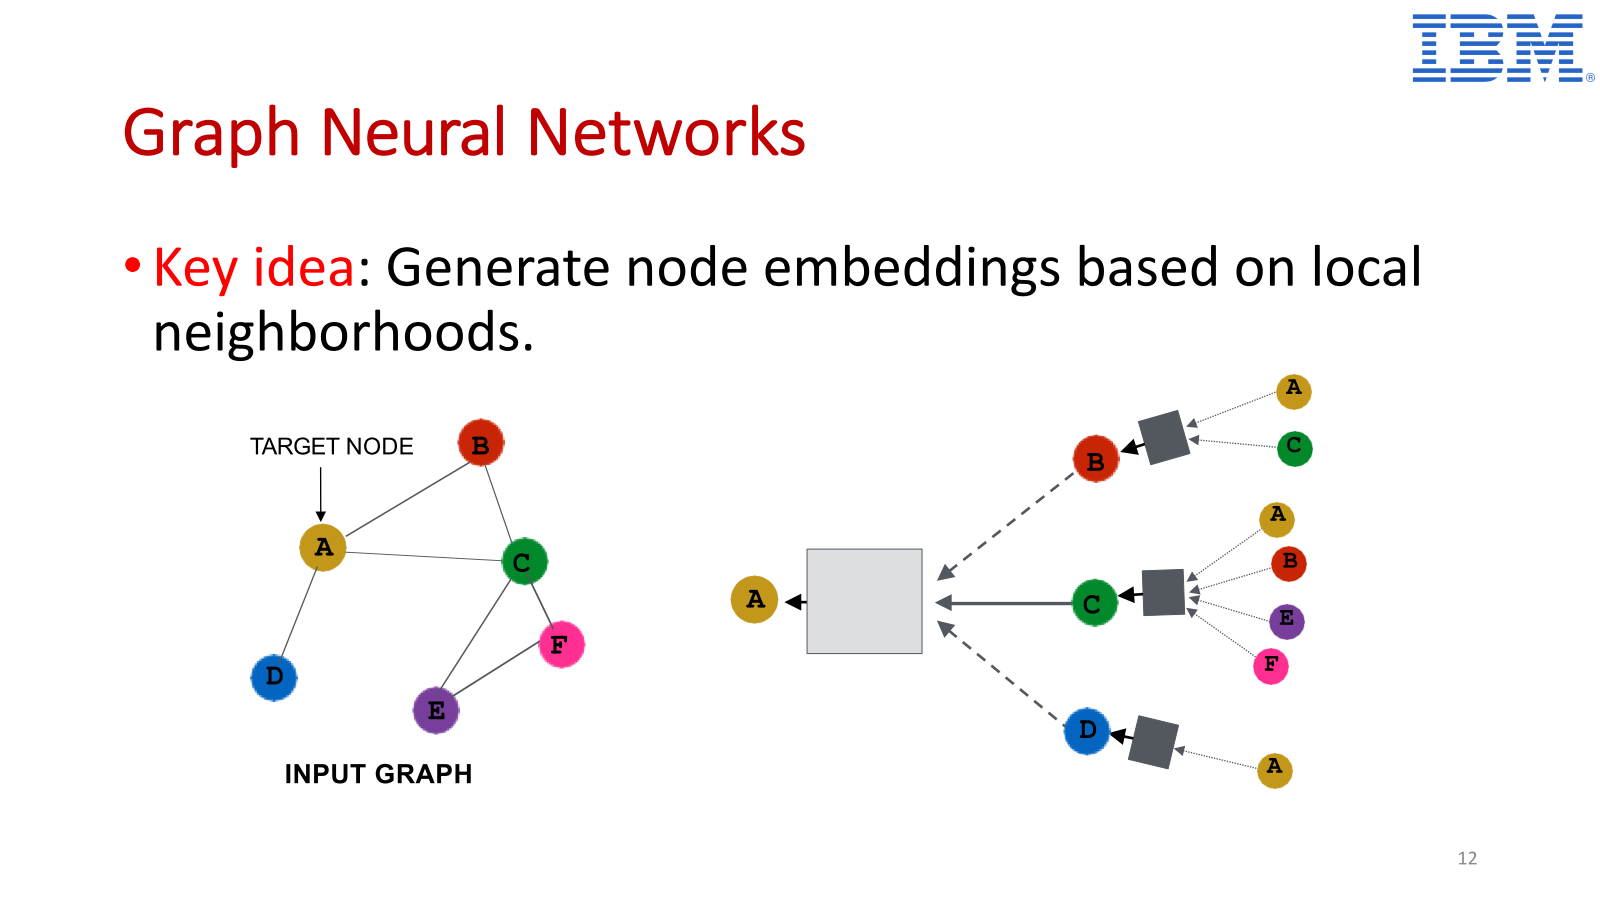
\includegraphics[width=\linewidth,keepaspectratio]{gnn30}
\end{center}	  

\end{frame}

%%%%%%%%%%%%%%%%%%%%%%%%%%%%%%%%%%%%%%%%%%%%%%%%%%%%%%%%%%%
\begin{frame}[fragile]\frametitle{}

\begin{center}
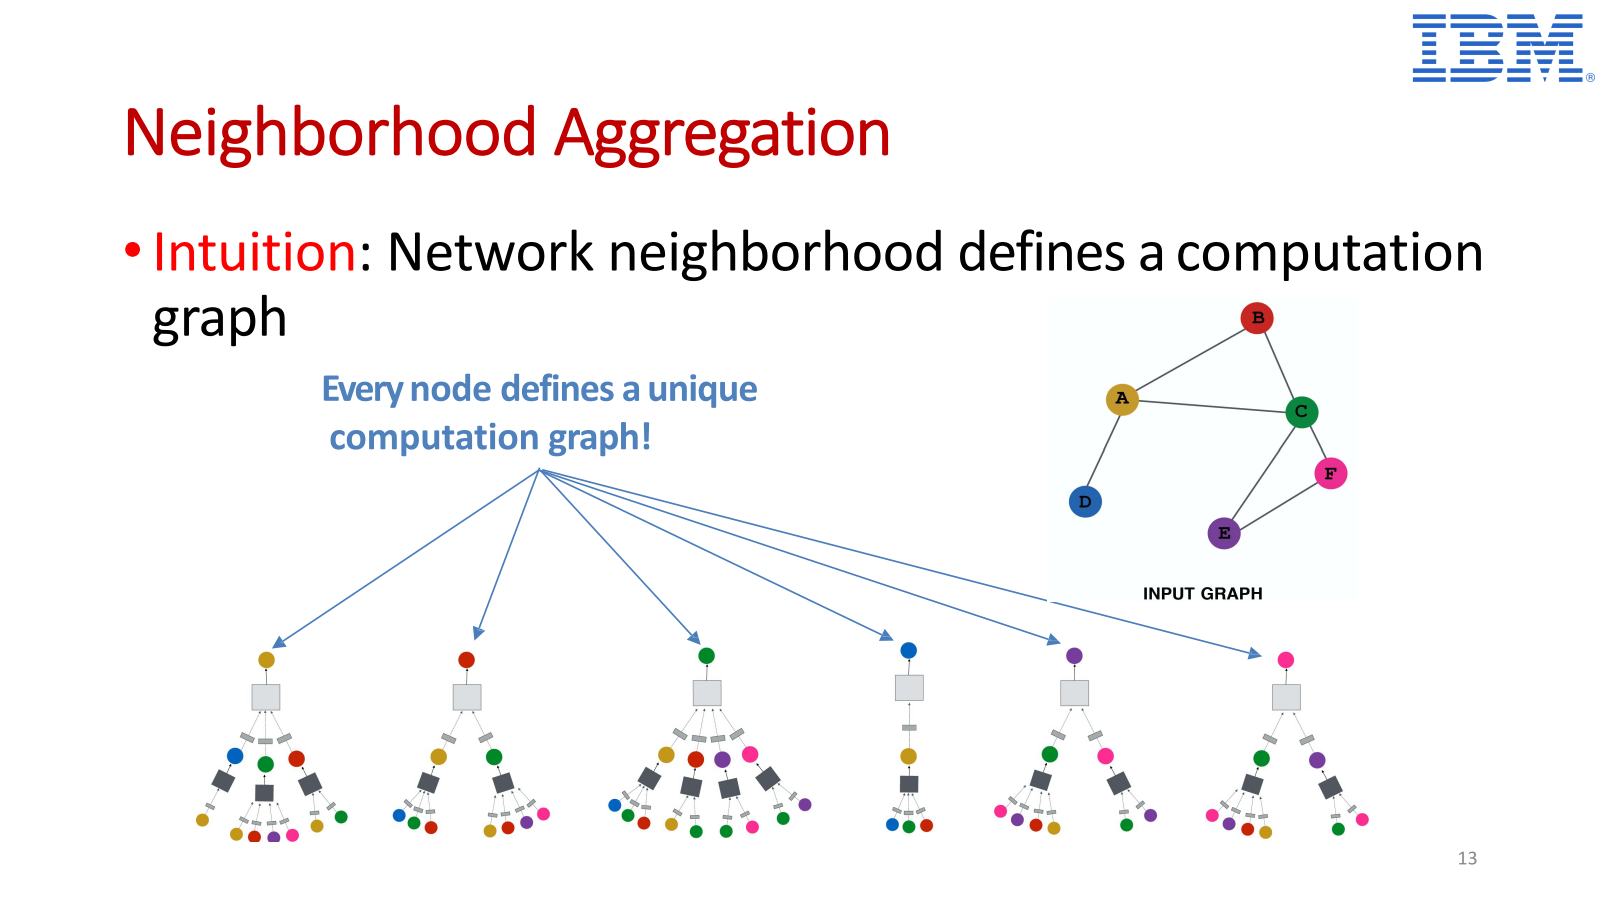
\includegraphics[width=\linewidth,keepaspectratio]{gnn31}
\end{center}	  

\end{frame}

%%%%%%%%%%%%%%%%%%%%%%%%%%%%%%%%%%%%%%%%%%%%%%%%%%%%%%%%%%%
\begin{frame}[fragile]\frametitle{}

\begin{center}
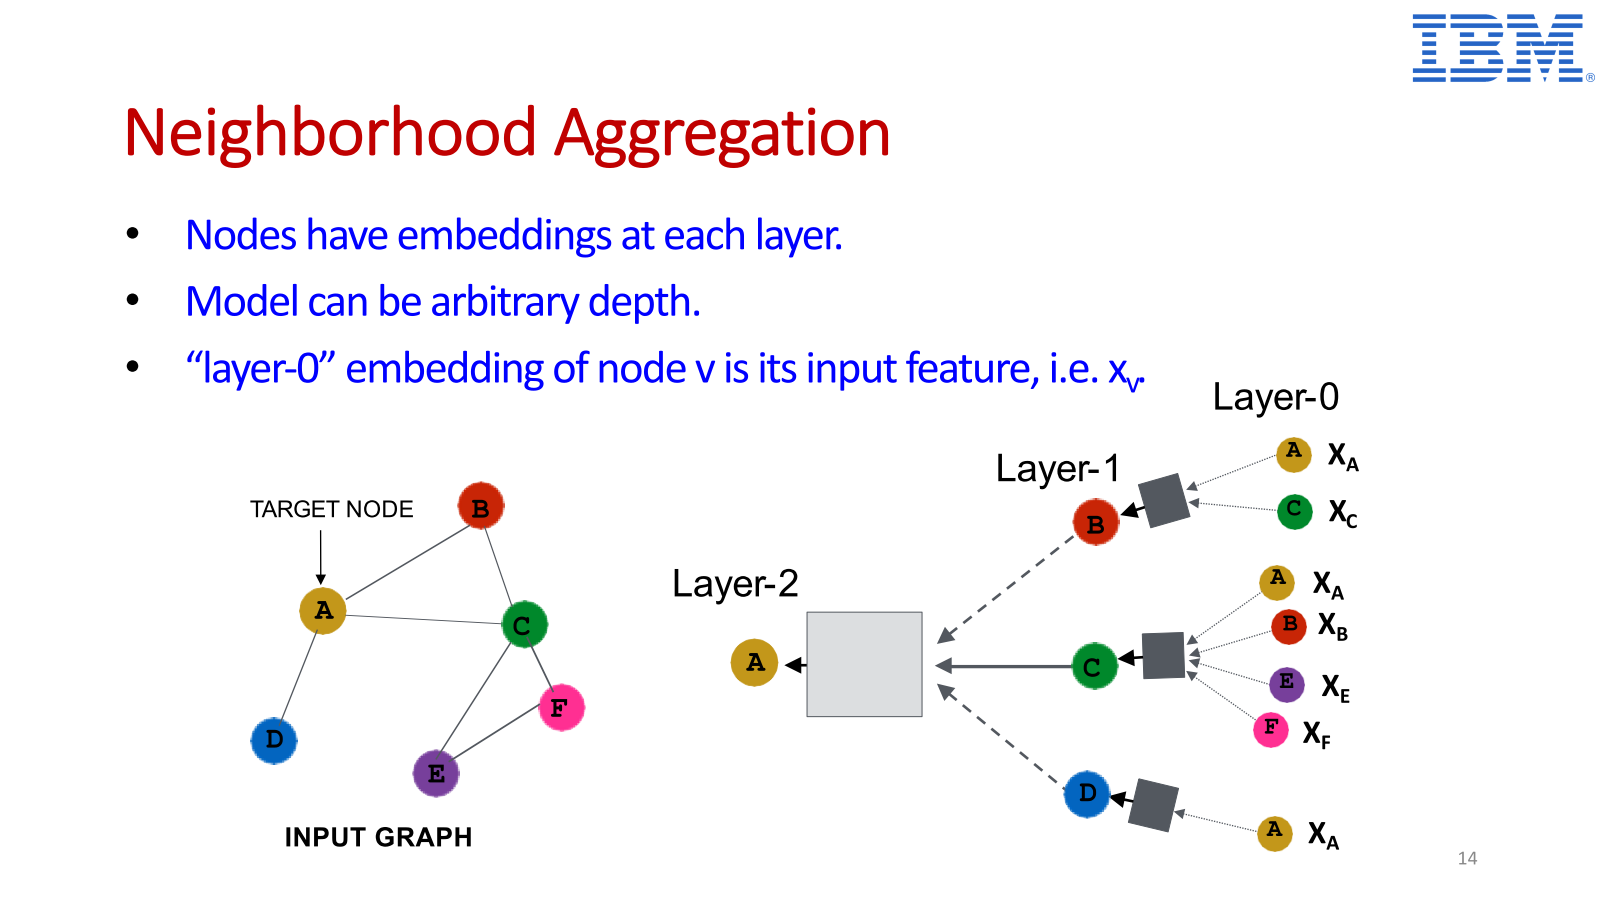
\includegraphics[width=\linewidth,keepaspectratio]{gnn32}
\end{center}	  

\end{frame}

%%%%%%%%%%%%%%%%%%%%%%%%%%%%%%%%%%%%%%%%%%%%%%%%%%%%%%%%%%%
\begin{frame}[fragile]\frametitle{}

\begin{center}
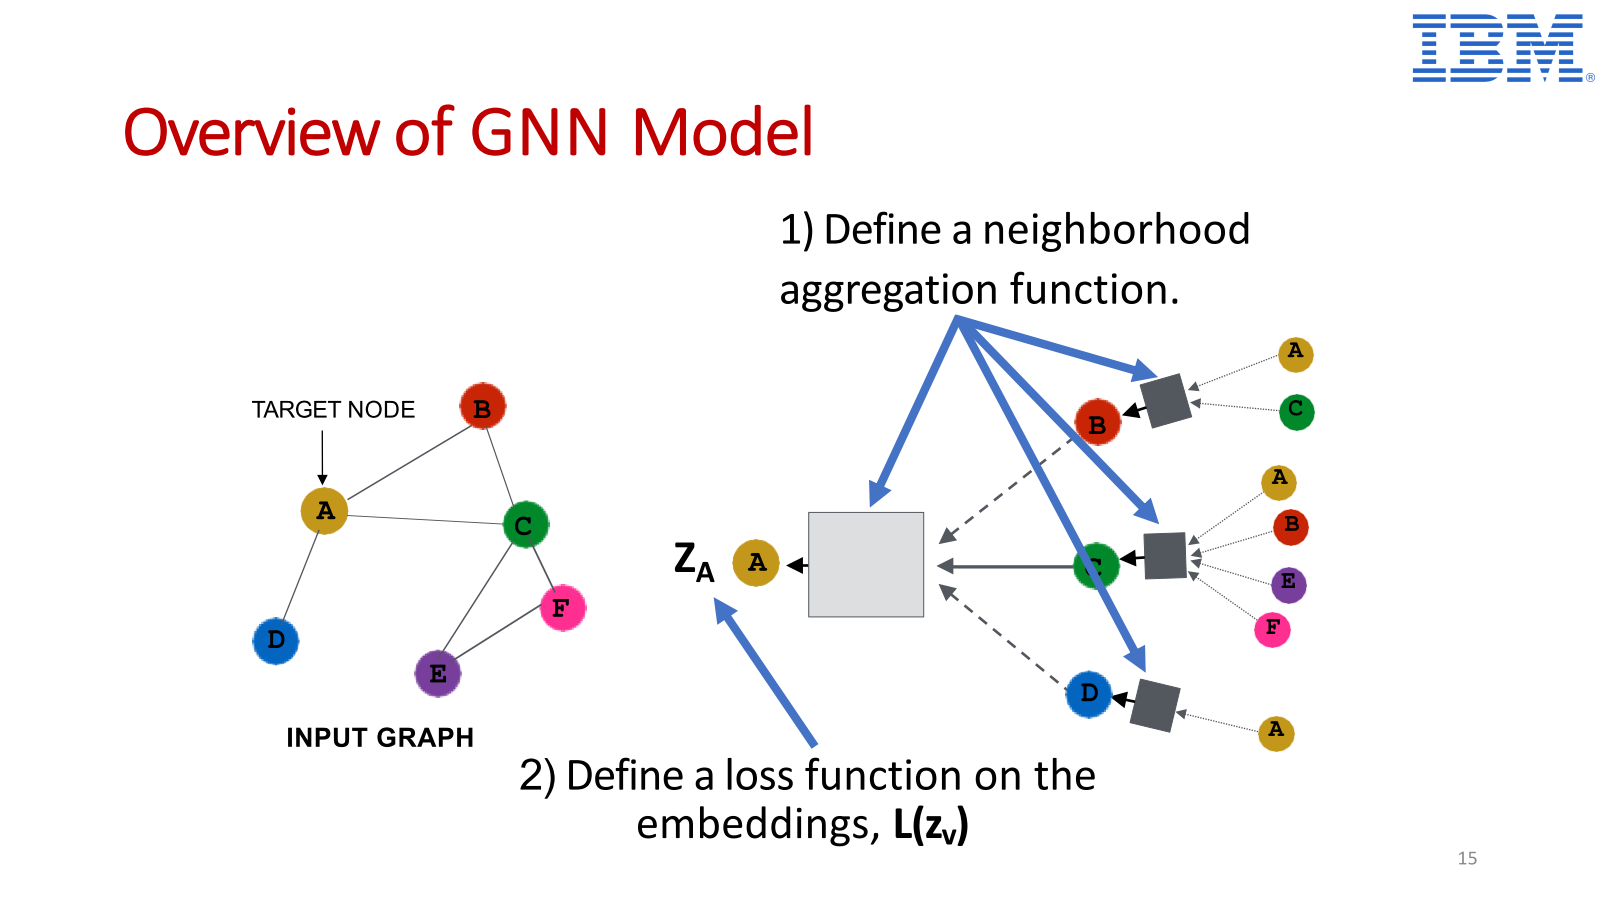
\includegraphics[width=\linewidth,keepaspectratio]{gnn33}
\end{center}	  

\end{frame}

%%%%%%%%%%%%%%%%%%%%%%%%%%%%%%%%%%%%%%%%%%%%%%%%%%%%%%%%%%%
\begin{frame}[fragile]\frametitle{}

\begin{center}
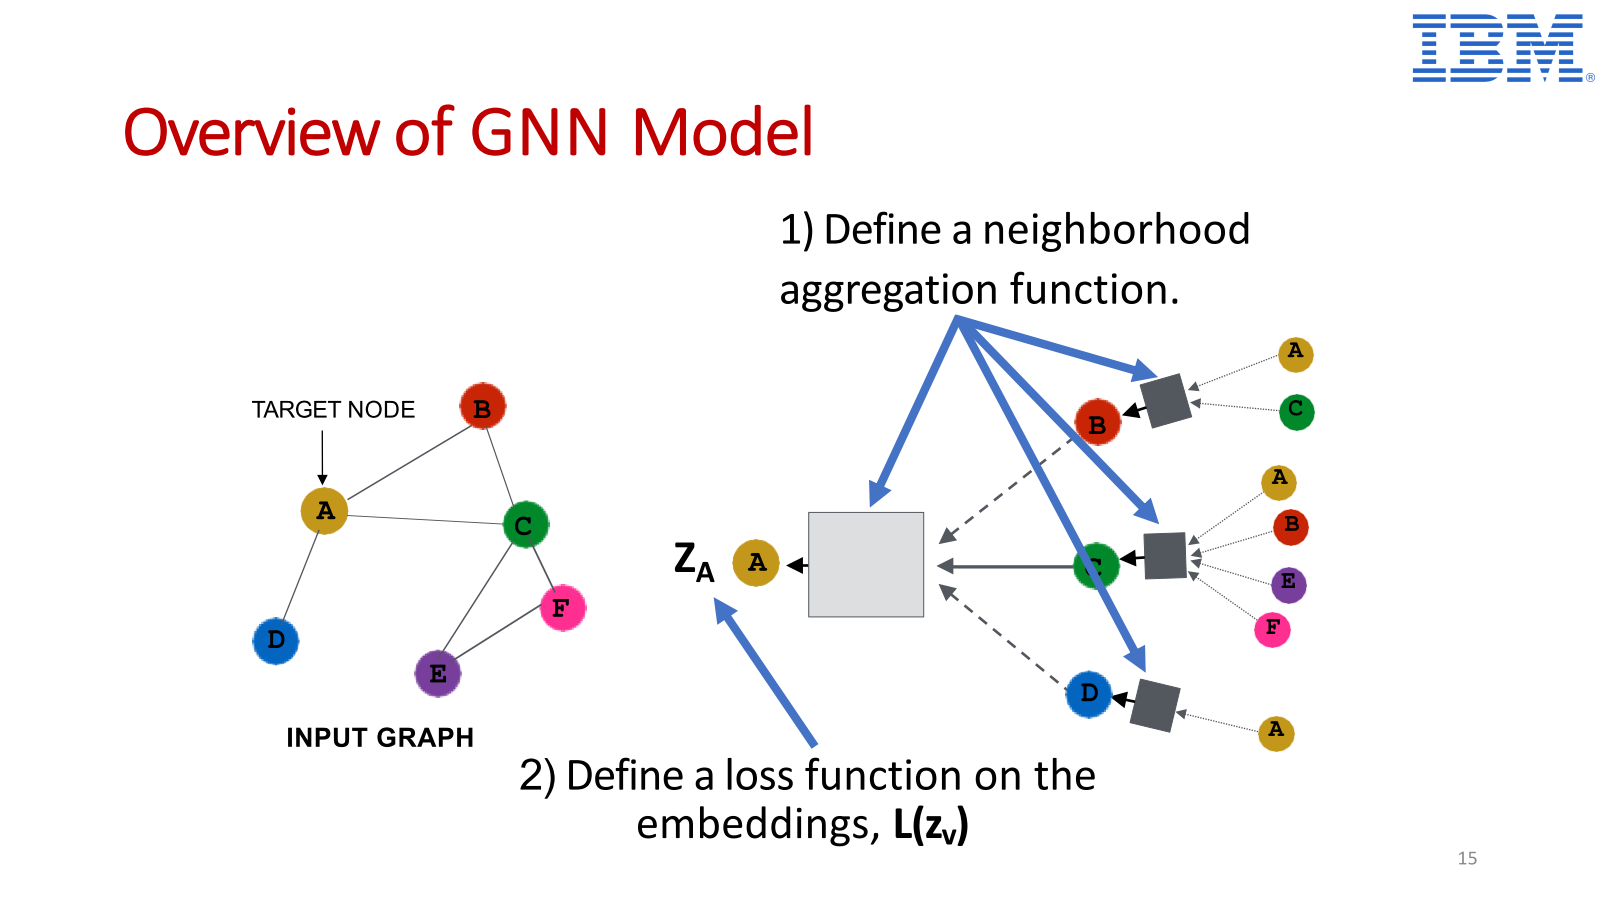
\includegraphics[width=\linewidth,keepaspectratio]{gnn34}
\end{center}	  

\end{frame}

%%%%%%%%%%%%%%%%%%%%%%%%%%%%%%%%%%%%%%%%%%%%%%%%%%%%%%%%%%%
\begin{frame}[fragile]\frametitle{}

\begin{center}
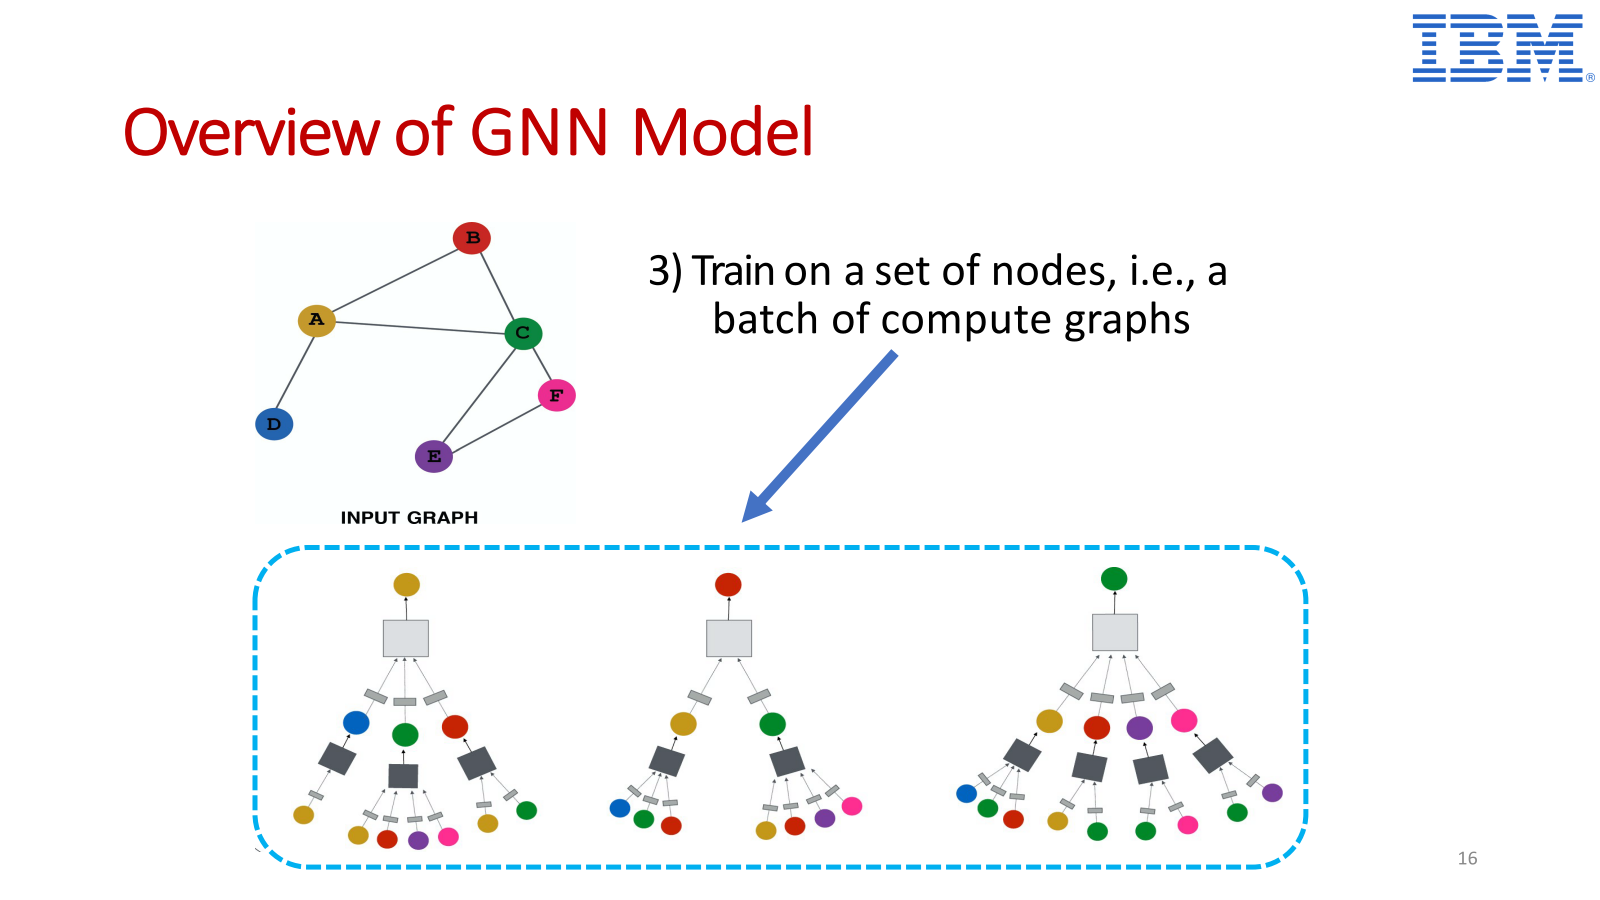
\includegraphics[width=\linewidth,keepaspectratio]{gnn35}
\end{center}	  

\end{frame}

%%%%%%%%%%%%%%%%%%%%%%%%%%%%%%%%%%%%%%%%%%%%%%%%%%%%%%%%%%%
\begin{frame}[fragile]\frametitle{}

\begin{center}
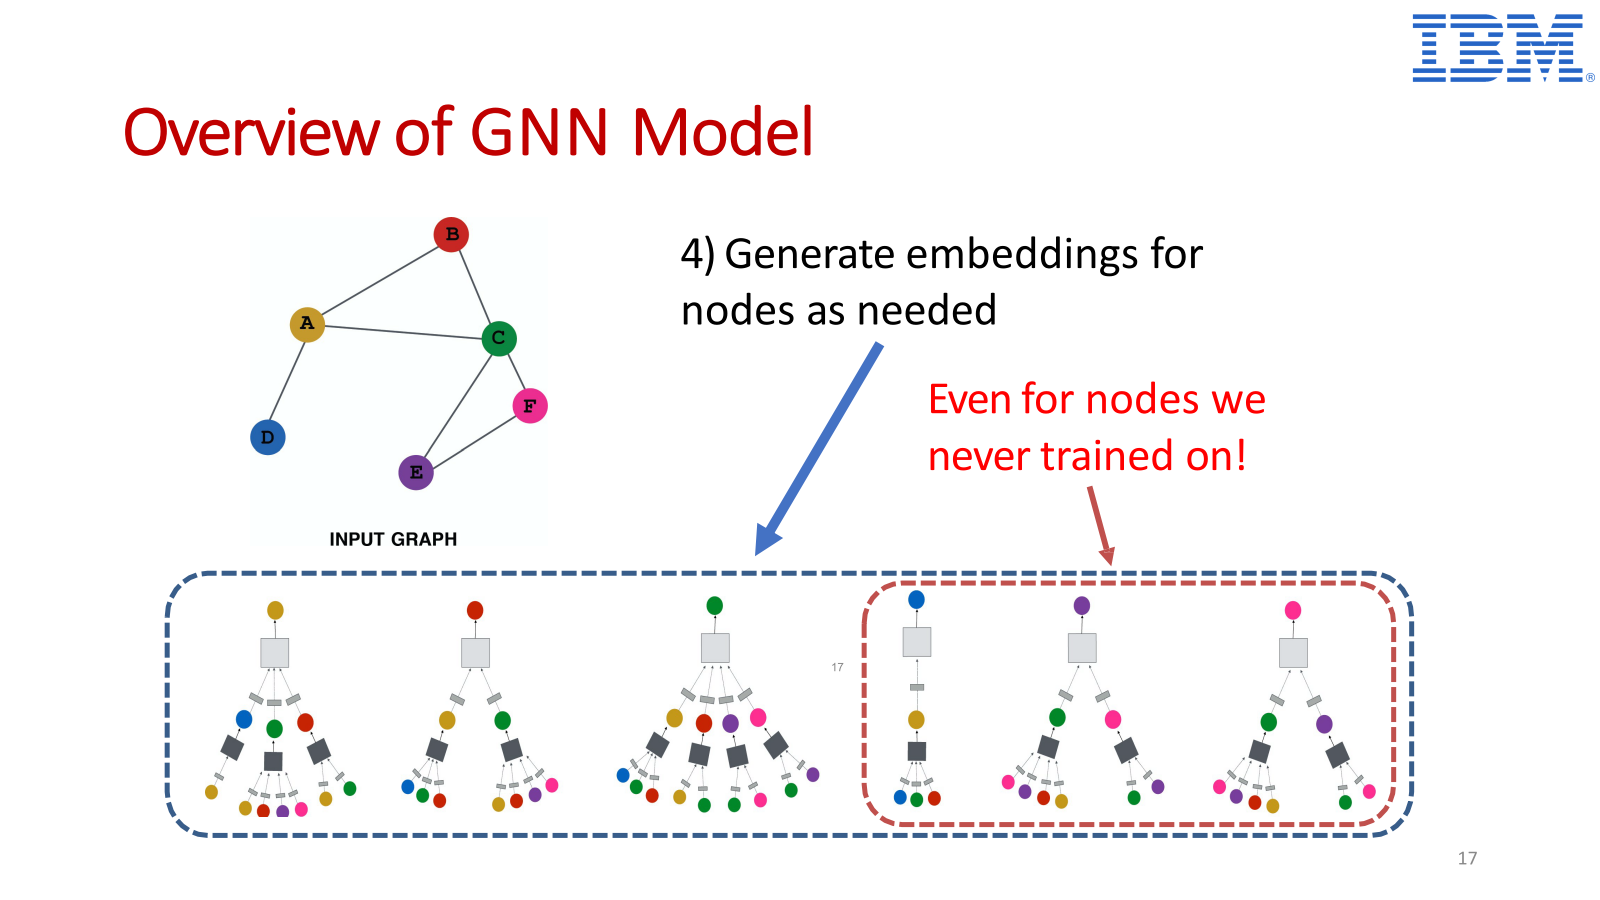
\includegraphics[width=\linewidth,keepaspectratio]{gnn36}
\end{center}	  

\end{frame}

%%%%%%%%%%%%%%%%%%%%%%%%%%%%%%%%%%%%%%%%%%%%%%%%%%%%%%%%%%%
\begin{frame}[fragile]\frametitle{}

\begin{center}
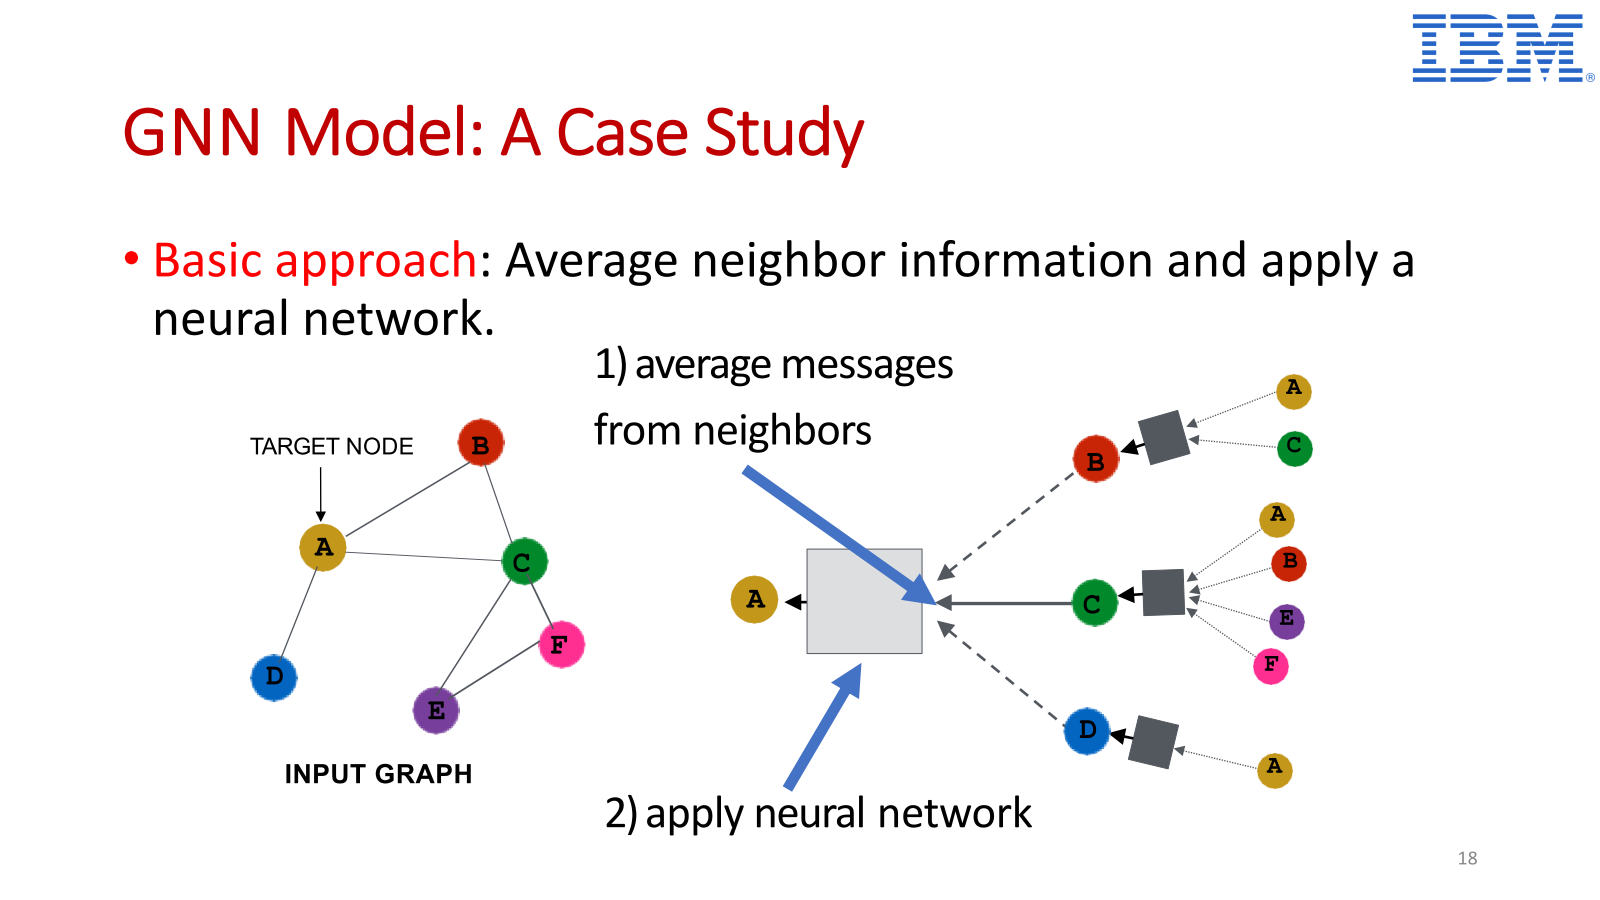
\includegraphics[width=\linewidth,keepaspectratio]{gnn37}
\end{center}	  

\end{frame}

%%%%%%%%%%%%%%%%%%%%%%%%%%%%%%%%%%%%%%%%%%%%%%%%%%%%%%%%%%%
\begin{frame}[fragile]\frametitle{}

\begin{center}
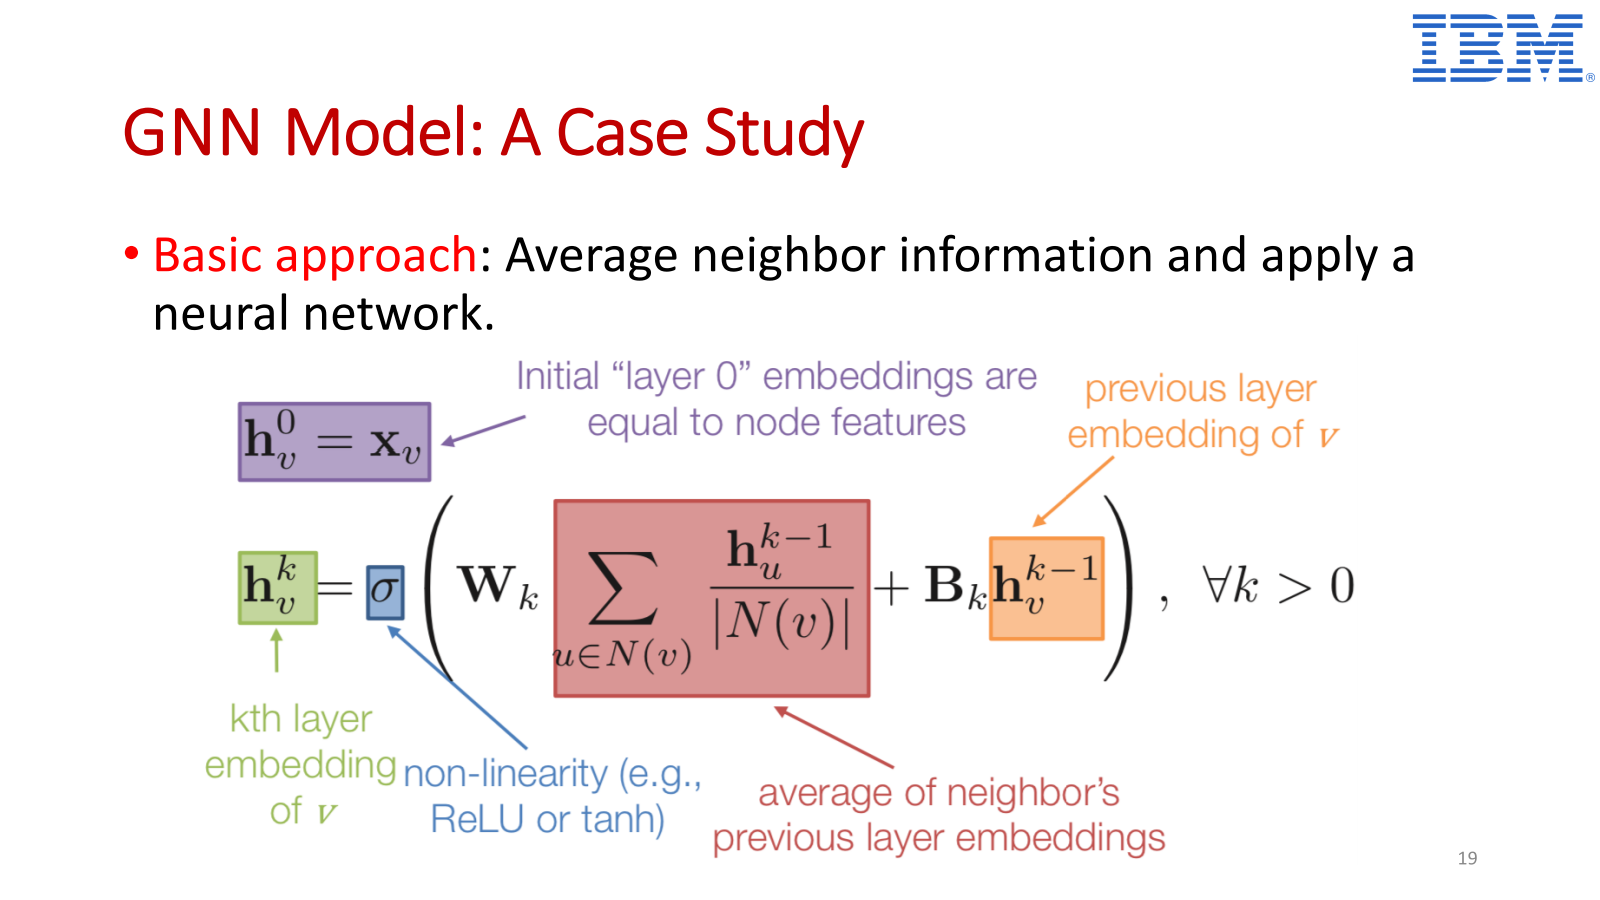
\includegraphics[width=\linewidth,keepaspectratio]{gnn38}
\end{center}	  

\end{frame}

%%%%%%%%%%%%%%%%%%%%%%%%%%%%%%%%%%%%%%%%%%%%%%%%%%%%%%%%%%%
\begin{frame}[fragile]\frametitle{}

\begin{center}
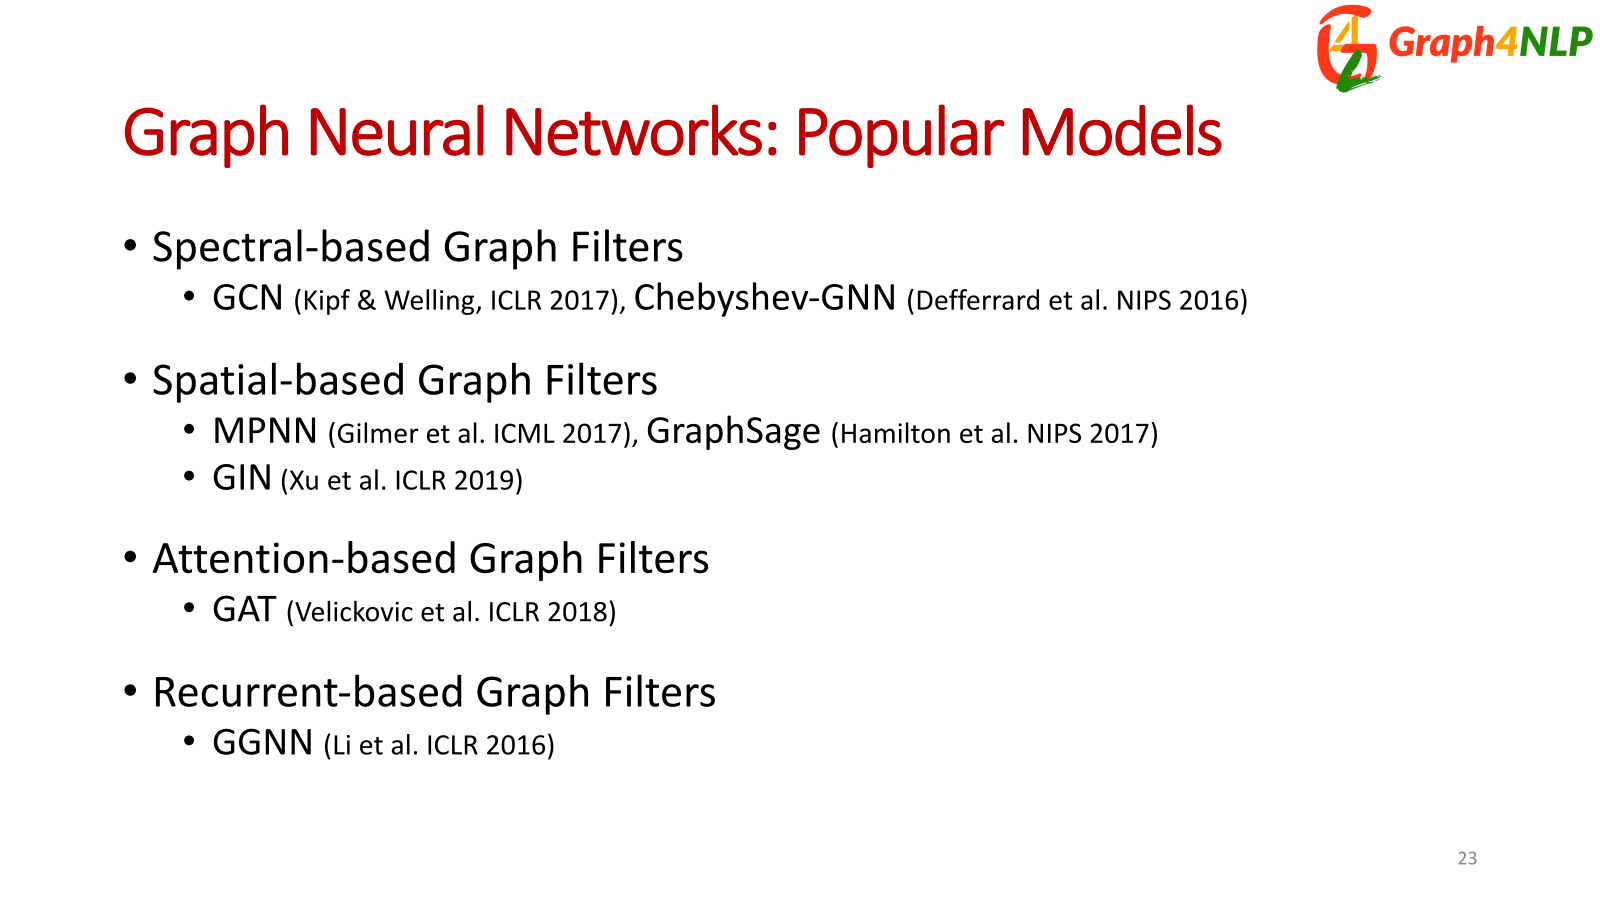
\includegraphics[width=\linewidth,keepaspectratio]{gnn39}
\end{center}	  

\end{frame}

%%%%%%%%%%%%%%%%%%%%%%%%%%%%%%%%%%%%%%%%%%%%%%%%%%%%%%%%%%%
\begin{frame}[fragile]\frametitle{Example 1: Graph convolution network (GCN)}

\begin{center}
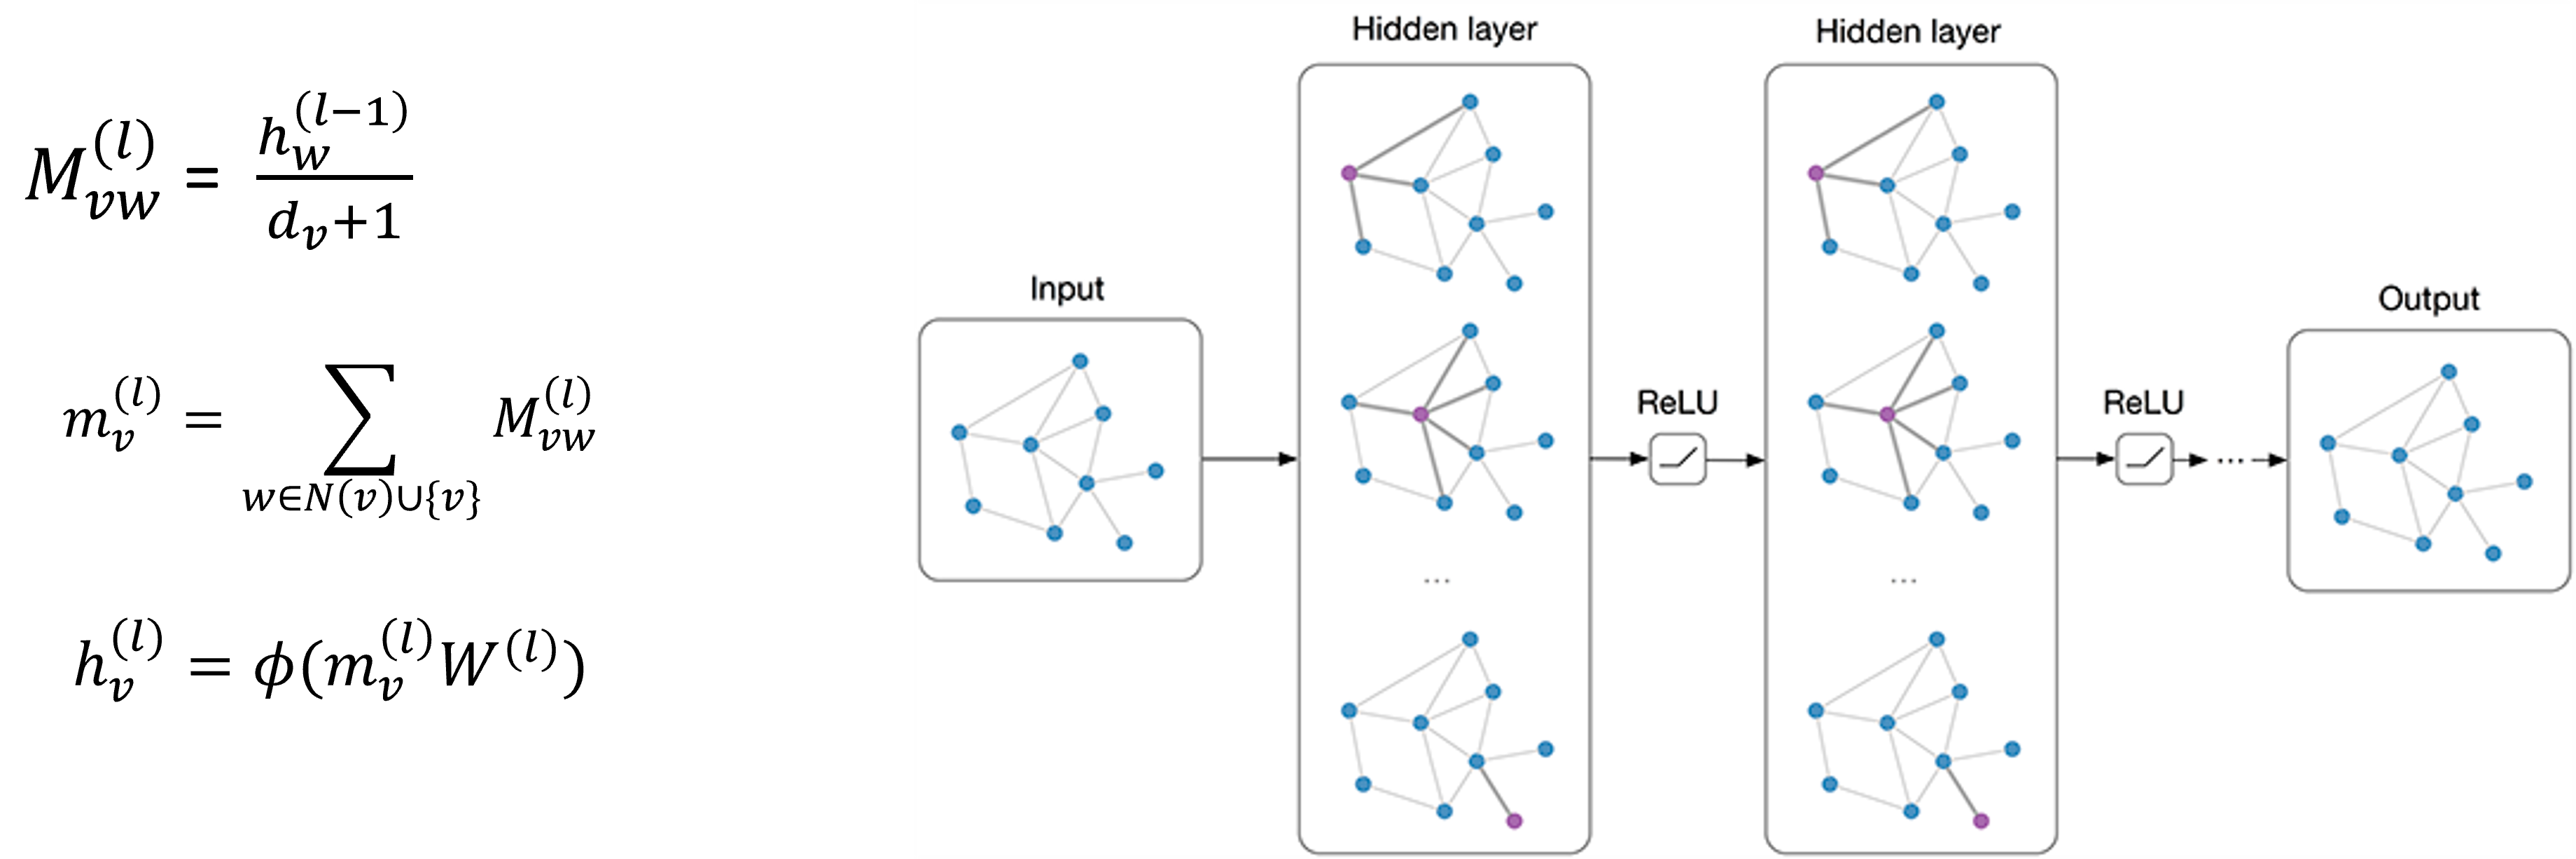
\includegraphics[width=\linewidth,keepaspectratio]{gnn40}
\end{center}	  

\end{frame}


%%%%%%%%%%%%%%%%%%%%%%%%%%%%%%%%%%%%%%%%%%%%%%%%%%%%%%%%%%%
\begin{frame}[fragile]\frametitle{Example 2: Graph attention networks (GAT)}

\begin{center}
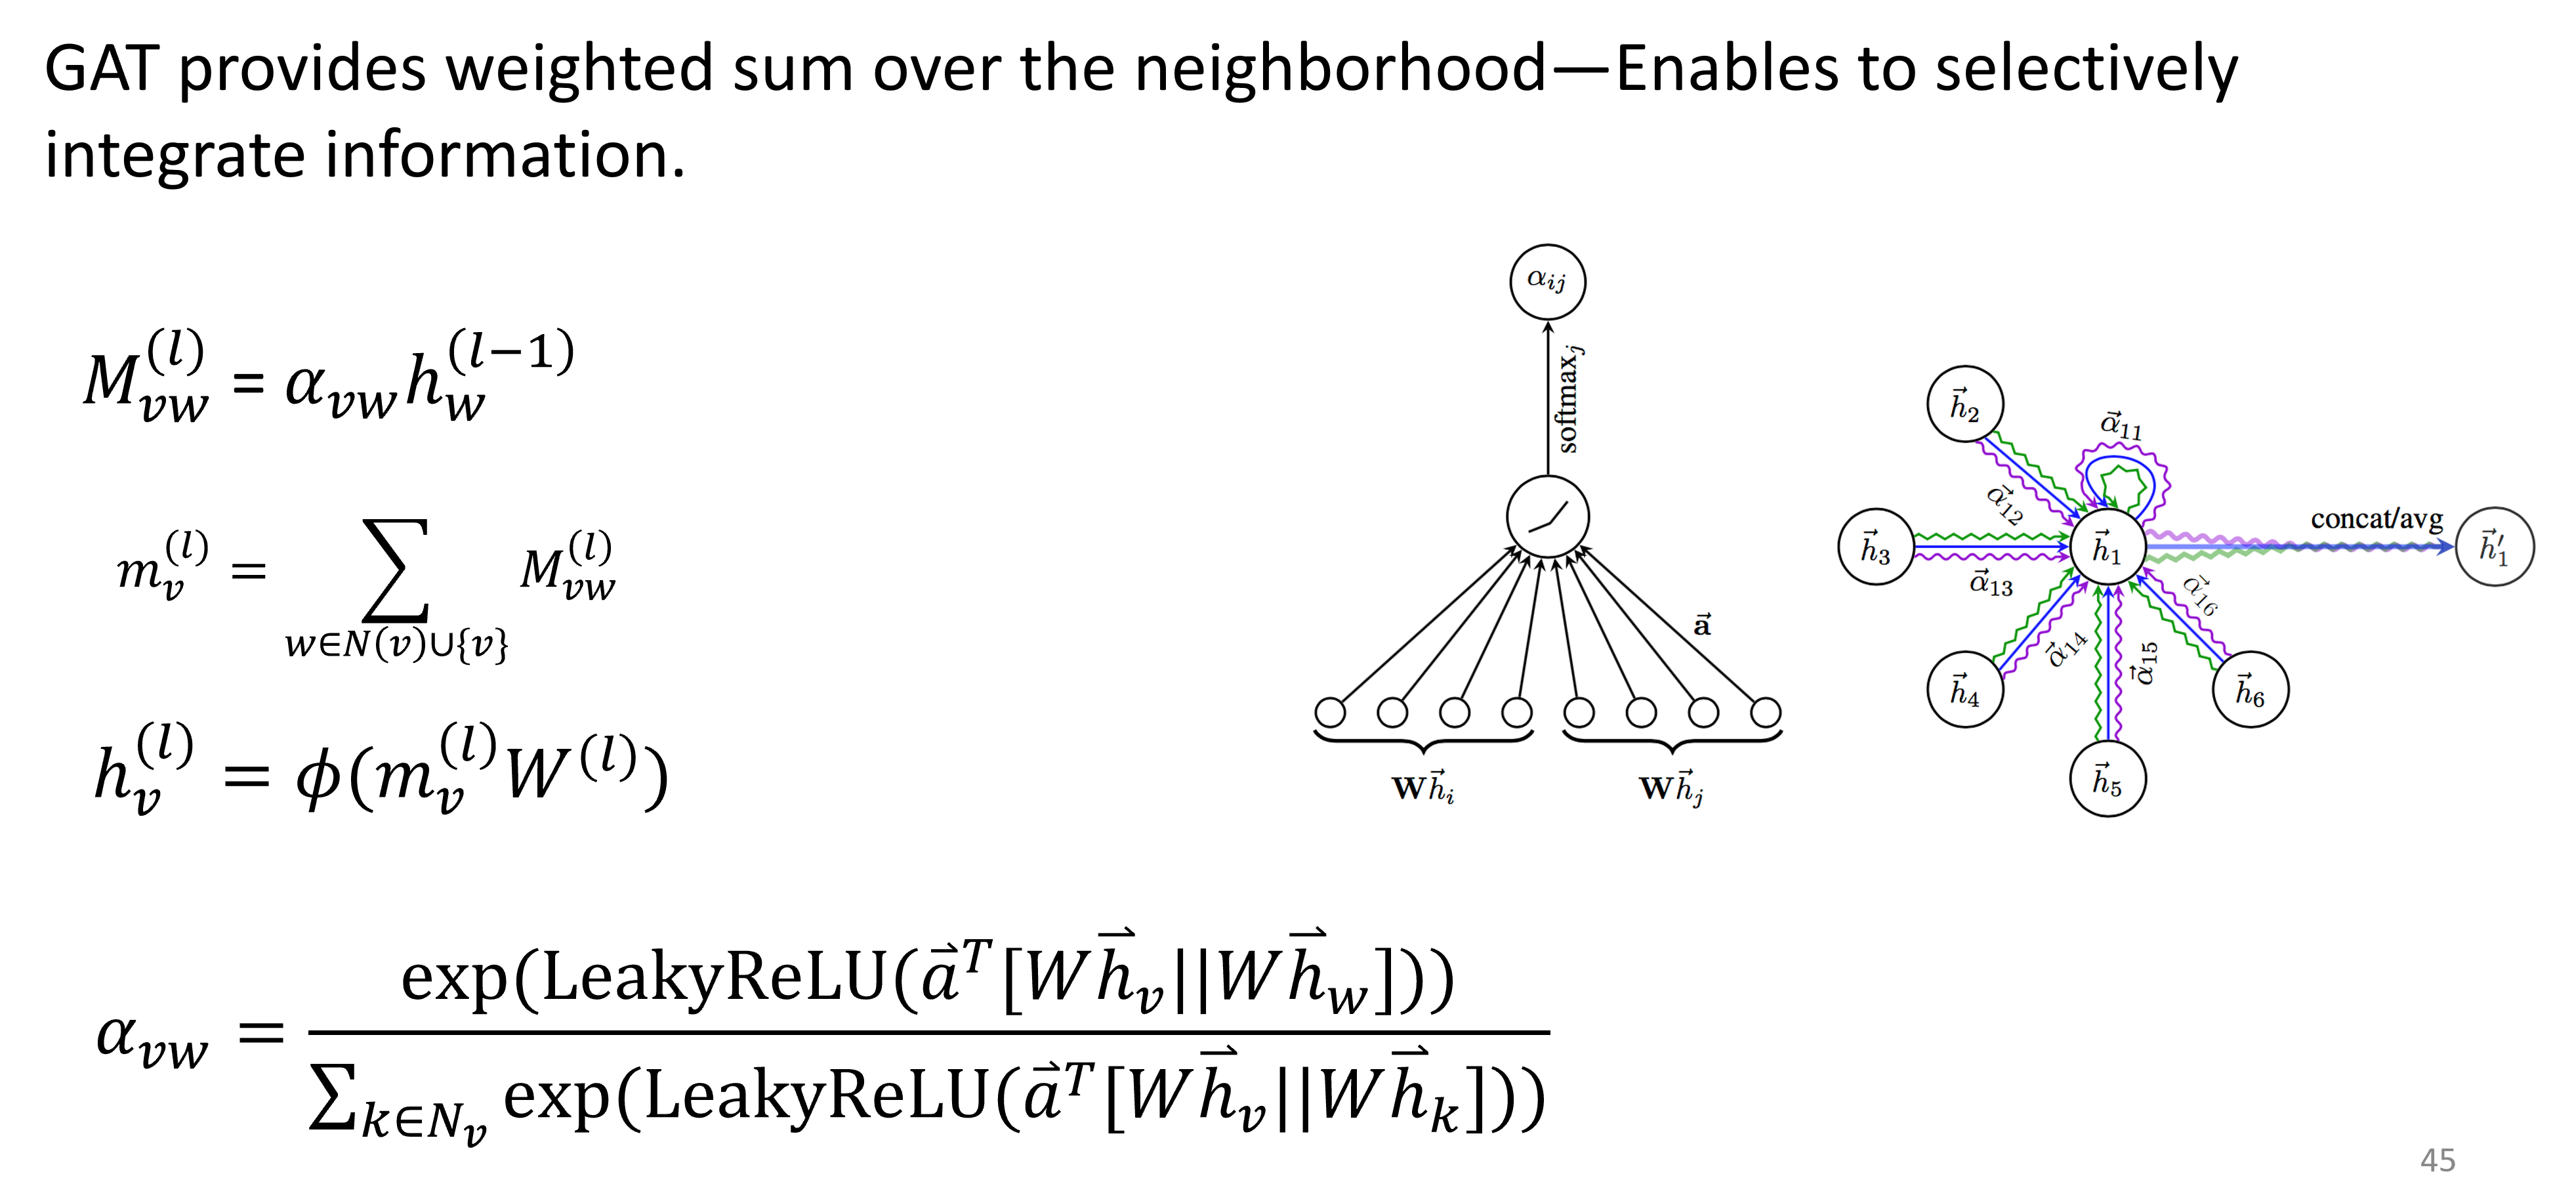
\includegraphics[width=\linewidth,keepaspectratio]{gnn41}
\end{center}	  

\end{frame}

%%%%%%%%%%%%%%%%%%%%%%%%%%%%%%%%%%%%%%%%%%%%%%%%%%%%%%%%%%%
\begin{frame}[fragile]\frametitle{Example 3: Relational graph convolution networks (RGCN)}

\begin{center}
\includegraphics[width=\linewidth,keepaspectratio]{gnn42}
\end{center}	  

\end{frame}

%%%%%%%%%%%%%%%%%%%%%%%%%%%%%%%%%%%%%%%%%%%%%%%%%%%%%%%%%%%
\begin{frame}[fragile]\frametitle{}

\begin{center}
\includegraphics[width=\linewidth,keepaspectratio]{gnn43}
\end{center}	  

\end{frame}

%%%%%%%%%%%%%%%%%%%%%%%%%%%%%%%%%%%%%%%%%%%%%%%%%%%%%%%%%%%
\begin{frame}[fragile]\frametitle{}

\begin{center}
\includegraphics[width=\linewidth,keepaspectratio]{gnn44}
\end{center}	  

\end{frame}

%%%%%%%%%%%%%%%%%%%%%%%%%%%%%%%%%%%%%%%%%%%%%%%%%%%%%%%%%%%
\begin{frame}[fragile]\frametitle{}

\begin{center}
\includegraphics[width=\linewidth,keepaspectratio]{gnn45}
\end{center}	  

\end{frame}

%%%%%%%%%%%%%%%%%%%%%%%%%%%%%%%%%%%%%%%%%%%%%%%%%%%%%%%%%%%
\begin{frame}[fragile]\frametitle{Why are graph neural networks better?}

GNNs compute node embeddings using both the structure of the graph and the features of the nodes and edges.


\begin{center}
\includegraphics[width=0.6\linewidth,keepaspectratio]{gnn46}
\end{center}	  

\end{frame}

%%%%%%%%%%%%%%%%%%%%%%%%%%%%%%%%%%%%%%%%%%%%%%%%%%%%%%%%%%%
\begin{frame}[fragile]\frametitle{Why are graph neural networks better?}

GNNs can integrate topologically distant information in a non-linear fashion. 



\begin{center}
\includegraphics[width=\linewidth,keepaspectratio]{gnn47}
\end{center}	  

\end{frame}

%%%%%%%%%%%%%%%%%%%%%%%%%%%%%%%%%%%%%%%%%%%%%%%%%%%%%%%%%%%
\begin{frame}[fragile]\frametitle{Why are graph neural networks better?}

GNNs and the downstream classification/regression models can be trained in an end-to-end fashion.


\begin{center}
\includegraphics[width=\linewidth,keepaspectratio]{gnn48}
\end{center}	  

\end{frame}

%%%%%%%%%%%%%%%%%%%%%%%%%%%%%%%%%%%%%%%%%%%%%%%%%%%%%%%%%%%
\begin{frame}[fragile]\frametitle{Why are graph neural networks better?}

GNNs are naturally inductive because they learn the same neural networks on all the nodes and edges.


\begin{center}
\includegraphics[width=0.8\linewidth,keepaspectratio]{gnn49}
\end{center}	  

\end{frame}

%%%%%%%%%%%%%%%%%%%%%%%%%%%%%%%%%%%%%%%%%%%%%%%%%%%%%%%%%%%
\begin{frame}[fragile]\frametitle{Summary}

\begin{itemize}
\item The solution to many applications can be formulated as graph learning problems.
\item Graph neural networks are a new technique for graph learning. They have multiple advantages over traditional methods.
\item GNNs are used in multiple graph tasks and can be trained end-to-end.
\end{itemize}

\end{frame}


\section[PyG]{PyTorch Geometric}
%%%%%%%%%%%%%%%%%%%%%%%%%%%%%%%%%%%%%%%%%%%%%%%%%%%%%%%%%%%%%%%%%%%%%%%%%%%%%%%%%%
\begin{frame}[fragile]\frametitle{}
\begin{center}
{\Large PyTorch Geometric}
\end{center}
\end{frame}


%%%%%%%%%%%%%%%%%%%%%%%%%%%%%%%%%%%%%%%%%%%%%%%%%%%%%%%%%%%
\begin{frame}[fragile]\frametitle{What is Pytorch Geometric (PyG)?}

\begin{itemize}
\item A python framework for deep learning on irregular structures like graphs, point clouds and manifolds, a.k.a Geometric Deep Learning 
\item Contains relational learning and 3D data processing methods such as Graph Neural Network(GNN)
\item Developed by Matthias Fey, eJan Eric Lenssn from TU Dortmund University. 
\item Functionalities provided:
	\begin{itemize}
	\item Neighbourhood Aggregation
	\item Global Pooling
	\item Hierarchical Pooling
	\item Mini-Batch Handling
	\item Processing of Datasets
	\end{itemize}
\end{itemize}

\end{frame}

%%%%%%%%%%%%%%%%%%%%%%%%%%%%%%%%%%%%%%%%%%%%%%%%%%%%%%%%%%%
\begin{frame}[fragile]\frametitle{Installation}

\begin{itemize}
\item Install PyTorch $>= 1.4.0$ via, say, \lstinline|conda install pytorch torchvision torchaudio cpuonly -c pytorch|
\item Note down Pytorch version: \lstinline|python -c "import torch; print(torch.__version__)"|
\item Note down CUDA version: \lstinline|python -c "import torch; print(torch.version.cuda)"|
\item Install dependencies (Replace TORCH with the PyTorch version and CUDA with the CUDA version, below)
\item Install PyG \lstinline|pip install torch-geometric|
\end{itemize}

\begin{lstlisting}
pip install torch-scatter -f https://pytorch-geometric.com/whl/torch-${TORCH}+${CUDA}.html
pip install torch-sparse -f https://pytorch-geometric.com/whl/torch-${TORCH}+${CUDA}.html
pip install torch-cluster -f https://pytorch-geometric.com/whl/torch-${TORCH}+${CUDA}.html
pip install torch-spline-conv -f https://pytorch-geometric.com/whl/torch-${TORCH}+${CUDA}.html 
\end{lstlisting}

\end{frame}

%%%%%%%%%%%%%%%%%%%%%%%%%%%%%%%%%%%%%%%%%%%%%%%%%%%%%%%%%%%
\begin{frame}[fragile]\frametitle{Representation}

Creating an unweighted and undirected graph with three nodes and four edges. 

\begin{center}
\includegraphics[width=0.3\linewidth,keepaspectratio]{pyg1}
\end{center}	  


\begin{lstlisting}
import torch
from torch_geometric.data import Data
edge_index = torch.tensor([[0, 1, 1, 2],
                            [1, 0, 2, 1]], dtype=torch.long)
x = torch.tensor([[-1], [0], [1]], dtype=torch.float)
data = Data(x=x, edge_index=edge_index) 
\end{lstlisting}

\end{frame}

%%%%%%%%%%%%%%%%%%%%%%%%%%%%%%%%%%%%%%%%%%%%%%%%%%%%%%%%%%%
\begin{frame}[fragile]\frametitle{Datasets}

PyG contains many benchmark datasets e.g., : all Planetoid datasets (Cora, Citeseer, Pubmed), all graph classification datasets from http://graphkernels.cs.tu-dortmund.de and their cleaned versions, etc


\begin{lstlisting}
from torch_geometric.datasets import TUDataset
dataset = TUDataset(root='/tmp/ENZYMES', name='ENZYMES')
\end{lstlisting}

\end{frame}

%%%%%%%%%%%%%%%%%%%%%%%%%%%%%%%%%%%%%%%%%%%%%%%%%%%%%%%%%%%
\begin{frame}[fragile]\frametitle{Data-loader}

PyG provides \lstinline|torch_geometric.data.DataLoader| for merging the data objects to a mini batch.

\begin{lstlisting}
from torch_geometric.datasets import TUDataset
from torch_geometric.data import DataLoader
dataset = TUDataset(root='/tmp/ENZYMES', name='ENZYMES', use_node_attr=True)
loader = DataLoader(dataset, batch_size=32, shuffle=True)
for batch in loader:
	 print(batch)
	 print(batch.num_graphs)
\end{lstlisting}

\end{frame}

%%%%%%%%%%%%%%%%%%%%%%%%%%%%%%%%%%%%%%%%%%%%%%%%%%%%%%%%%%%
\begin{frame}[fragile]\frametitle{Data-Transform}

PyG provides its data transformation utility whose input is Data object and output is transformed Data object.

\begin{lstlisting}
import torch_geometric.transforms as T
from torch_geometric.datasets import ShapeNet
dataset = ShapeNet(root='/tmp/ShapeNet', categories=['Airplane'],
									 pre_transform=T.KNNGraph(k=6))
dataset[0] 
\end{lstlisting}

\end{frame}

%%%%%%%%%%%%%%%%%%%%%%%%%%%%%%%%%%%%%%%%%%%%%%%%%%%%%%%%%%%
\begin{frame}[fragile]\frametitle{Graph Neural Network Definition}

Create a two-layer GCN network.

\begin{lstlisting}
import torch
import torch.nn.functional as F
from torch_geometric.nn import GCNConv
class Net(torch.nn.Module):
	 def __init__(self):
			 super(Net, self).__init__()
			 self.conv1 = GCNConv(dataset.num_node_features, 16)
			 self.conv2 = GCNConv(16, dataset.num_classes)
	 def forward(self, data):
			 x, edge_index = data.x, data.edge_index
			 x = self.conv1(x, edge_index)
			 x = F.relu(x)
			 x = F.dropout(x, training=self.training)
			 x = self.conv2(x, edge_index)
			 return F.log_softmax(x, dim=1) 
\end{lstlisting}

\end{frame}
%%%%%%%%%%%%%%%%%%%%%%%%%%%%%%%%%%%%%%%%%%%%%%%%%%%%%%%%%%%
\begin{frame}[fragile]\frametitle{Training and Evaluation}

Let’s train this model on the train nodes for 200 epochs.

\begin{lstlisting}
device = torch.device('cuda' if torch.cuda.is_available() else 'cpu')
model = Net().to(device)
data = dataset[0].to(device)
optimizer = torch.optim.Adam(model.parameters(), lr=0.01, weight_decay=5e-4)
model.train()
for epoch in range(200):
	 optimizer.zero_grad()
	 out = model(data)
	 loss = F.nll_loss(out[data.train_mask], data.y[data.train_mask])
	 loss.backward()
	 optimizer.step() 
	 
# Evaluate the model on test data.
model.eval()
_, pred = model(data).max(dim=1)
correct = int(pred[data.test_mask].eq(data.y[data.test_mask]).sum().item())
acc = correct / int(data.test_mask.sum())
print('Accuracy: {:.4f}'.format(acc)) 	 
\end{lstlisting}

\end{frame}


%%%%%%%%%%%%%%%%%%%%%%%%%%%%%%%%%%%%%%%%%%%%%%%%%%%%%%%%%%%
\begin{frame}[fragile]\frametitle{References}
Slides primarily borrowed from \ldots

\begin{itemize}
\item Overview of Graph Neural Networks - George Karypis
\item Graph Neural Networks: Models and Applications - Yao Ma, et al
\item GraphSAGE: Deep Learning for Relational Data - Jure Leskovec
\item Deep Learning on Graphs in Natural Language Processing and Computer Vision - Lingfei Wu, IBM Research AI
\item Deep Learning on Graphs for Natural Language Processing - Lingfei Wu, Yu Chen, Heng Ji, and Yunyao Li, NAACL-2021 Tutorial
\item Hands-On Guide to PyTorch Geometric (With Python Code) - Aishwarya Verma
\end{itemize}

\end{frame}
